%%%%%%%%%%%%%%%%%%%%%%%%%%%%%%%%%%%%%%%%%
% Beamer Presentation
% LaTeX Template
% Version 1.0 (10/11/12)
%
% This template has been downloaded from:
% http://www.LaTeXTemplates.com
%
% License:
% CC BY-NC-SA 3.0 (http://creativecommons.org/licenses/by-nc-sa/3.0/)
%
%%%%%%%%%%%%%%%%%%%%%%%%%%%%%%%%%%%%%%%%%

%----------------------------------------------------------------------------------------
%	PACKAGES AND THEMES
%----------------------------------------------------------------------------------------

\documentclass[aspectratio=169]{beamer}

\mode<presentation> {


\definecolor{LightBlue}{RGB}{93,111,122}
\definecolor{TitleCopper}{RGB}{0,108,92}
\definecolor{emphasis}{RGB}{212,0,0}
\definecolor{darkgreen}{rgb}{0,0.5,0}
% The Beamer class comes with a number of default slide themes
% which change the colors and layouts of slides. Below this is a list
% of all the themes, uncomment each in turn to see what they look like.

\usetheme{Madrid}
% Change base colour beamer@blendedblue (originally RGB: 0.2,0.2,0.7)
\colorlet{beamer@blendedblue}{red!80!black}

% As well as themes, the Beamer class has a number of color themes
% for any slide theme. Uncomment each of these in turn to see how it
% changes the colors of your current slide theme.

%\setbeamertemplate{footline} % To remove the footer line in all slides uncomment this line
%\setbeamertemplate{footline}[page number] % To replace the footer line in all slides with a simple slide count uncomment this line

%\setbeamertemplate{navigation symbols}{} % To remove the navigation symbols from the bottom of all slides uncomment this line
}

\newcommand\Fontvi{\fontsize{10}{10}\selectfont}
\newcommand{\norm}[1]{\left\lVert#1\right\rVert_2}
\newcommand{\abs}[1]{\left|#1\right|}
\newcommand\emphasis[1]{{\textbf{\color{emphasis}#1}}}

% Toggle animations on or off for faster build times
\newif\ifshowanimations
\showanimationstrue
% \showanimationsfalse

% Toggle animations on or off for faster build times
\newif\ifshowcitations
\showcitationstrue
% \showcitationsfalse

% for zero-padded image numbers inside animations
\newcommand\zeropad[2]{%
  \ifnum#2<0\relax%
    {\ensuremath-}\zeropadA{#1}{\the\numexpr#2*-1\relax}%
  \else%
    \zeropadA{#1}{#2}%
  \fi%
}
\def\zeropadA#1#2{%
  \ifnum1#2<1#1
    \zeropadA{#1}{0#2}%
  \else%
    #2%
  \fi%
}

%==============================================================================%
%% Mathematical symbols

\newcommand{\Ti}{\mbox{$T_1$}}
\newcommand{\nh}{\mbox{$n_\text{hidden}$}}
\newcommand{\Pd}{\mbox{$P_\text{dropout}$}}
\newcommand{\nl}{\mbox{$n_\text{layers}$}}
\newcommand{\Pt}{\mbox{$P_\text{teacher}$}}
\newcommand{\lr}{\mbox{$l_\text{rate}$}}
\newcommand{\bs}{\mbox{$b_\text{size}$}}
\newcommand{\R}{\mbox{$\lambda$}}
\newcommand{\e}{\mbox{$\epsilon$}}
\newcommand{\etol}{\mbox{$\epsilon_\text{tol}$}}
\newcommand{\fs}{\mbox{$f_\text{sample}$}}
\newcommand{\ff}{\mbox{$f_\text{features}$}}
\newcommand{\D}{\mbox{$D$}}
\newcommand{\ns}{\mbox{$n_\text{stages}$}}
\newcommand{\nd}{\mbox{$n_\text{degree}$}}

\newcommand{\To}{\mbox{$T_2$}}
\newcommand{\np}{\mbox{$n_\text{patience}$}}
\newcommand{\nepoch}{\mbox{$n_\text{epochs}$}}
\newcommand{\nbest}{\mbox{$n_\text{epochs}^\text{best}$}}

%==============================================================================%
%% Bibliography settings
\ifshowcitations
	\usepackage[backend=biber,autocite=footnote,citestyle=authoryear,style=mla,maxcitenames=10]{biblatex}

	\newcommand*{\volnumpunct}{\addcomma\space}
	\renewcommand*{\newunitpunct}{\addcomma\space}
	\renewcommand*{\subtitlepunct}{\nopunct\space}
	\renewcommand*{\intitlepunct}{\nopunct\addspace}
	\renewcommand*{\relatedpunct}{\addsemicolon\space}
	\renewcommand*{\finentrypunct}{} 

	\renewcommand*{\bibfootnotewrapper}[1]{\bibsentence #1} % remove final period

	\DeclareCiteCommand{\footpartcite}[\mkbibfootnote]{
		{
			\boolfalse{citetracker} % not sure if this helps
			\usebibmacro{prenote}
		}%
		{\usebibmacro{citeindex}%
			\setunit{\addcomma}
			% \printnames{labelname}%
			% \setunit{\labelnamepunct}
			\printnames[default]{author} % default ordering first name, last name
			\newunit
			\printfield{year}
			\newunit
			{\color{emphasis}\printfield{journaltitle}}
		}
		{\usebibmacro{postnote}}
		\vspace{-1.5em}
	}

	\AtEveryCitekey{\iffootnote{\color{emphasis}\tiny}{\color{blue}}}

	\makeatletter
	\renewcommand\@makefnmark{\textsuperscript{\@thefnmark}} % suppress ref mark
	\renewcommand\@makefntext[1]{\tiny\noindent{[\@thefnmark]}#1} % smaller font size
	\makeatother

	\usepackage{filecontents}
	\addbibresource{informs_presentation.bib}
	% \renewcommand*{\thefootnote}{\alph{footnote}} % alpha footnotes
\fi
%==============================================================================%
%% Footer formatting

\setbeamertemplate{footline}
{
	\leavevmode%
	\hbox{%
	\begin{beamercolorbox}[wd=.2\paperwidth,ht=2.25ex,dp=1ex,center]{author in head/foot}%
	\usebeamerfont{author in head/foot}\insertshortauthor
	\end{beamercolorbox}%
	\begin{beamercolorbox}[wd=.6\paperwidth,ht=2.25ex,dp=1ex,center]{title in head/foot}%
	\usebeamerfont{title in head/foot}{\href{https://khbalhandawi.github.io/}{https://khbalhandawi.github.io/}}
	\end{beamercolorbox}%
	\begin{beamercolorbox}[wd=.2\paperwidth,ht=2.25ex,dp=1ex,center]{date in head/foot}%
	\insertdate~~\insertframenumber{} / \inserttotalframenumber\hspace*{1ex}
	\end{beamercolorbox}}%
	\vskip0pt%
}

\usepackage{textpos}
\addtobeamertemplate{frametitle}{}{%
	\begin{textblock*}{100mm}(.94\textwidth,-1.1cm)
		\colorbox{white}{
\includegraphics[height=1.2cm]{logos/mcgill_logo.pdf}}
	\end{textblock*}
}

%==============================================================================%
%% Reduce TOC spacing

\makeatletter
\patchcmd{\beamer@sectionintoc}{\vskip1.5em}{\vskip0.5em}{}{}
\makeatother

%==============================================================================%
%% Good behaving itemize env with top aligned columns

\makeatletter
\newenvironment{myitemize}{%
   \setlength{\topsep}{0pt}
   \setlength{\partopsep}{0pt}
   \renewcommand*{\@listi}{\leftmargin\leftmargini \parsep\z@ \topsep\z@ \itemsep\z@}
   \let\@listI\@listi
   \itemize
}{\enditemize}
\makeatother  

%==============================================================================%
%% Imported packages

\usepackage{changepage} % adjust slide margins
\usepackage{graphicx} % Allows including images
\usepackage{animate} % For animated images
\graphicspath{ {images/} }
\usepackage{tikz}

\usepackage{tikz}
\usepackage{tikz-dimline}
\usetikzlibrary{calc,fadings,positioning,arrows,shapes,backgrounds,shapes.geometric,arrows.meta}
\tikzfading[name=fade r,right color=transparent!100,left color=transparent!0]
\tikzstyle{every picture}+=[remember picture]
\tikzstyle{na} = [baseline=-.5ex]
% this "frames" a rectangle node
\newcommand\framenode[2][10pt]{
    \fill[white,path fading=fade r] (#2.south west) rectangle ($(#2.north west)+( #1,0)$);
}
\newcommand{\fixedpicture}[4]{ % height, content
    \node (TRSschematic) at ( [xshift = #1, yshift = #2] current page.center) %or: (current page.west
	{\includegraphics[height=#3]{#4}};
}
\newcommand{\tikzmark}[3][]{\tikz[remember picture,baseline] \node [anchor=base,#1](#2) {$#3$};}


\usepackage{tabularx}
\usepackage{multirow}% tables
\usepackage{booktabs} % Allows the use of \toprule, \midrule and \bottomrule in tables
\newcolumntype{L}[1]{>{\raggedright\let\newline\\\arraybackslash\hspace{0pt}}m{#1}}
\newcolumntype{C}[1]{>{\centering\let\newline\\\arraybackslash\hspace{0pt}}m{#1}}
\newcolumntype{R}[1]{>{\raggedleft\let\newline\\\arraybackslash\hspace{0pt}}m{#1}}

\usepackage{lmodern} % load a font with all the characters
\usepackage{amssymb}
\usepackage{amsmath}
%\usepackage{unicode-math}
\usepackage{cmbright}
%\SetSymbolFont{largesymbols}{normal}{OMX}{iwona}{m}{n}

\usepackage{cleveref}% reference multiple equations
\usepackage{caption}
\usepackage{subcaption}
\usepackage{enumitem} % tick and cross bullet points
\usepackage{amsfonts}
\usepackage{ragged2e} % justify text
\usepackage{multido} % loop over i images
\usepackage{array} % for tables 
\usepackage{varwidth} % for bullets inside tikz nodes
\usepackage{fancybox} % for rounded boxes
\usepackage{xstring} % for string lookup functions 

\usepackage{pifont} % for ding commands
\newcommand{\cmark}{\ding{51}} % for check marks
\newcommand{\xmark}{\ding{55}} % for cross marks
\usepackage{bbding,enumitem} % tick and cross bullet points

\newlength{\mytextsize} % fontsize length for animations inline
%This part fails.... 
\makeatletter
	\setlength{\mytextsize}{\f@size pt}
\makeatother

\setitemize{label=\usebeamerfont*{itemize item}% Restore original beamer style
\usebeamercolor[fg]{itemize item}
\usebeamertemplate{itemize item}}

\setbeamerfont{block body}{size=\scriptsize}
\setbeamerfont{block body alerted}{size=\scriptsize}
\setbeamerfont{block body example}{size=\scriptsize}
\captionsetup{textfont={scriptsize,it},labelformat=empty,labelsep=none}
\usepackage{multicol} % multiple columns for itemize lists

% INTEGRATED PROBLEM BLOCK %
\setbeamercolor{block title}{fg=white,bg=blue}
\setbeamercolor{block body}{fg=black, bg=blue!20!white}

% INTEGRATED PROBLEM BLOCK %
\setbeamercolor{block title}{fg=white,bg=blue}
\setbeamercolor{block body}{fg=black, bg=blue!20!white}

% INTEGRATED PROBLEM BLOCK %
\newenvironment<>{blueblock}[1]{%
\setbeamercolor{itemize item}{fg=blue}
\setbeamercolor{block title}{fg=white,bg=blue}
\setbeamercolor{block body}{fg=black, bg=blue!20!white}
	\begin{block}#2{#1}}{\end{block}}

% TITLE BLOCK %
\newenvironment<>{titleblock}[1]{%
\setbeamercolor{block title}{fg=black,bg=red!20!white}
\setbeamercolor{block body}{fg=black, bg=red!20!white}
	\begin{block}#2{#1}}{\end{block}}

% well behaved centering environment
\newenvironment{nscenter}
 {\parskip=0pt\par\nopagebreak\centering}
 {\par\noindent\ignorespacesafterend}

% Image scales and sizes
\newlength\imagewidth
\newlength\imagescale
\pgfmathsetlength{\imagewidth}{6cm}
\pgfmathsetlength{\imagescale}{\imagewidth/600}

% https://tex.stackexchange.com/a/28633
\makeatletter
% Use Euclid's Algorithm to find the greatest 
% common divisor of two integers.
\def\gcd#1#2{{% #1 = a, #2 = b
    \ifnum#2=0 \edef\next{#1}\else
        \@tempcnta=#1 \@tempcntb=#2 \divide\@tempcnta by\@tempcntb
        \multiply\@tempcnta by\@tempcntb  % q*b
        \@tempcntb=#1
        \advance\@tempcntb by-\@tempcnta % remainder in \@tempcntb
        \ifnum\@tempcntb=0
            \@tempcnta=#2
            \ifnum\@tempcnta < 0 \@tempcnta=-\@tempcnta\fi
            \xdef\gcd@next{\noexpand%
                \def\noexpand\thegcd{\the\@tempcnta}}%
        \else
            \xdef\gcd@next{\noexpand\gcd{#2}{\the\@tempcntb}}%
        \fi
    \fi}\gcd@next
}
\newcommand\reduceFrac[2]
{%
   \gcd{#1}{#2}{\@tempcnta=#1 \divide\@tempcnta by\thegcd
   \@tempcntb=#2 \divide\@tempcntb by\thegcd
   \ifnum\@tempcntb<0\relax
      \@tempcntb=-\@tempcntb
        \@tempcnta=-\@tempcnta
    \fi
    \xdef\rfNumer{\the\@tempcnta}
    \xdef\rfDenom{\the\@tempcntb}}%
}
\makeatother

\newcommand*{\fracReduced}[2]{%
    \reduceFrac{#1}{#2}%
    \ensuremath{%
        \ifnum\rfDenom=1
            \rfNumer
        \else
            \frac{\rfNumer}{\rfDenom}%
        \fi
    }%
}%


\newcommand{\addfraction}[2]{% 1N, 1D, 2N, 2D
    \pgfmathsetmacro{\newnumerator}{#1}
    \pgfmathsetmacro{\newdenominator}{#2}
    \pgfmathtruncatemacro{\newnumeratorTrunc}{\newnumerator}
    \pgfmathtruncatemacro{\newdenominatorTrunc}{\newdenominator}
    \pgfkeys{/pgf/number format/.cd,int detect,precision=2}
    \fracReduced{\newnumeratorTrunc}{\newdenominatorTrunc}
}
%----------------------------------------------------------------------------------------
%	TITLE PAGE
%----------------------------------------------------------------------------------------

\title[]{Modeling and Optimization of Public Health Policy-Making for Epidemics} % The short title appears at the bottom of every slide, the full title is only on the title page

\author[INFORMS Healthcare]{Dr. Khalil Al Handawi} % Your name

\institute[McGill]% Your institution as it will appear on the bottom of every slide, may be shorthand to save space
{
	~\\
	\textit{\small
	2023 INFORMS Healthcare Conference\\} % Your institution for the title page
}
\date{July 26, 2023} % Date, can be changed to a custom date

\begin{document}

\begin{frame}
	\begin{tikzpicture}[remember picture,overlay]
	\node[opacity=0.9] (image) at
		([xshift=-0.125\textwidth, yshift =-1cm]current page.east) 	%or: (current page.center)
		{
\includegraphics[height=1.6\textheight]{logos/mcgill_logo.pdf}};
		\framenode[600pt]{image}
\end{tikzpicture}

\titlepage % Print the title page as the first slide
\end{frame}

%----------------------------------------------------------------------------------------
% \begin{frame}
% \frametitle{Overview} % Table of contents slide, comment this block out to remove it
% \tableofcontents[hideallsubsections] % Throughout your presentation, if you choose to use \section{} and \subsection{} commands, these will automatically be printed on this slide as an overview of your presentation
% \end{frame}
%----------------------------------------------------------------------------------------

%------------------------------------------------
\section{Introduction on epidemiology}
%------------------------------------------------
\begin{frame}[t]
	\frametitle{Research displinces in epidemiology}
	\tikzstyle{background grid}=[draw, black!50,step=.5cm]
	%
	Forecasting novel epidemics is a multidisciplinary field involving multiple \emph{targets} \ifshowcitations\footpartcite{Wu2021}\fi\\
	~\\
	\begin{columns}
		\begin{column}{0.5\textwidth}
			In the early stages of epidemics, we have access to:\\
			%
			\begin{itemize}
				\item<2-> \only<2>{\emphasis}{Social behaviour and demographics}
				\item<3-> \only<3>{\emphasis}{Incidence rate data}
			\end{itemize}
			%
			Simulation models can be developed based on this information and used in \only<4>{\emphasis}{public health and social measures (PHSMs)} policy-making.
		\end{column}
		\begin{column}{0.5\textwidth}
			\begin{tikzpicture}[remember picture, overlay] %show background grid, 
				% Put the graphic inside a node. This makes it easy to place the
				% graphic and to draw on top of it. 
				% The above right option is used to place the lower left corner
				% of the image at the (0,0) coordinate. 
				\node [inner sep=0pt,above left, opacity=1.0]  at (0.99\textwidth,-0.5\textheight) (targets) 
					{
						\only<1>{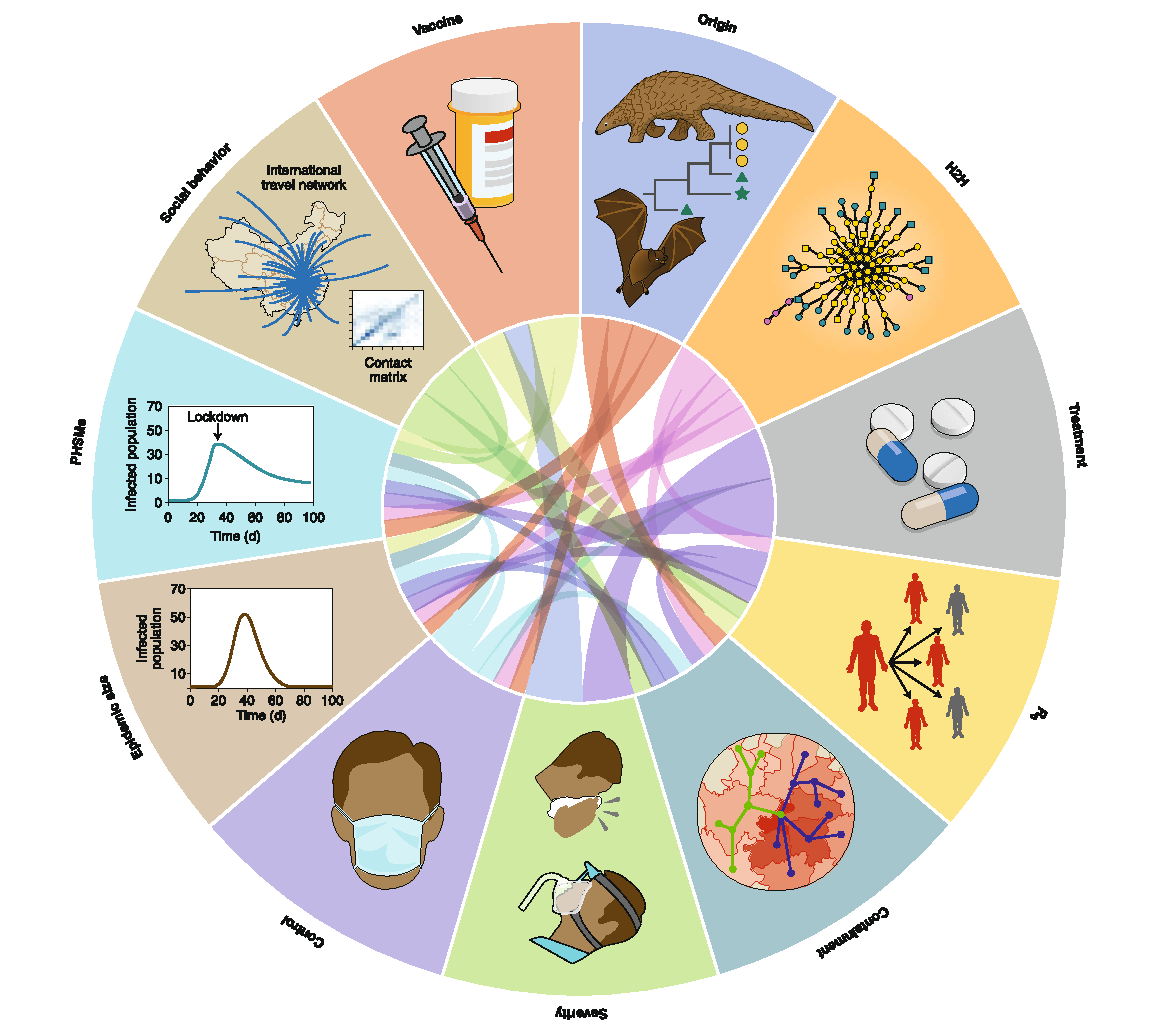
\includegraphics[width=0.9\textwidth]{targets/nowcasting_targets_1.pdf}}%
						\only<2>{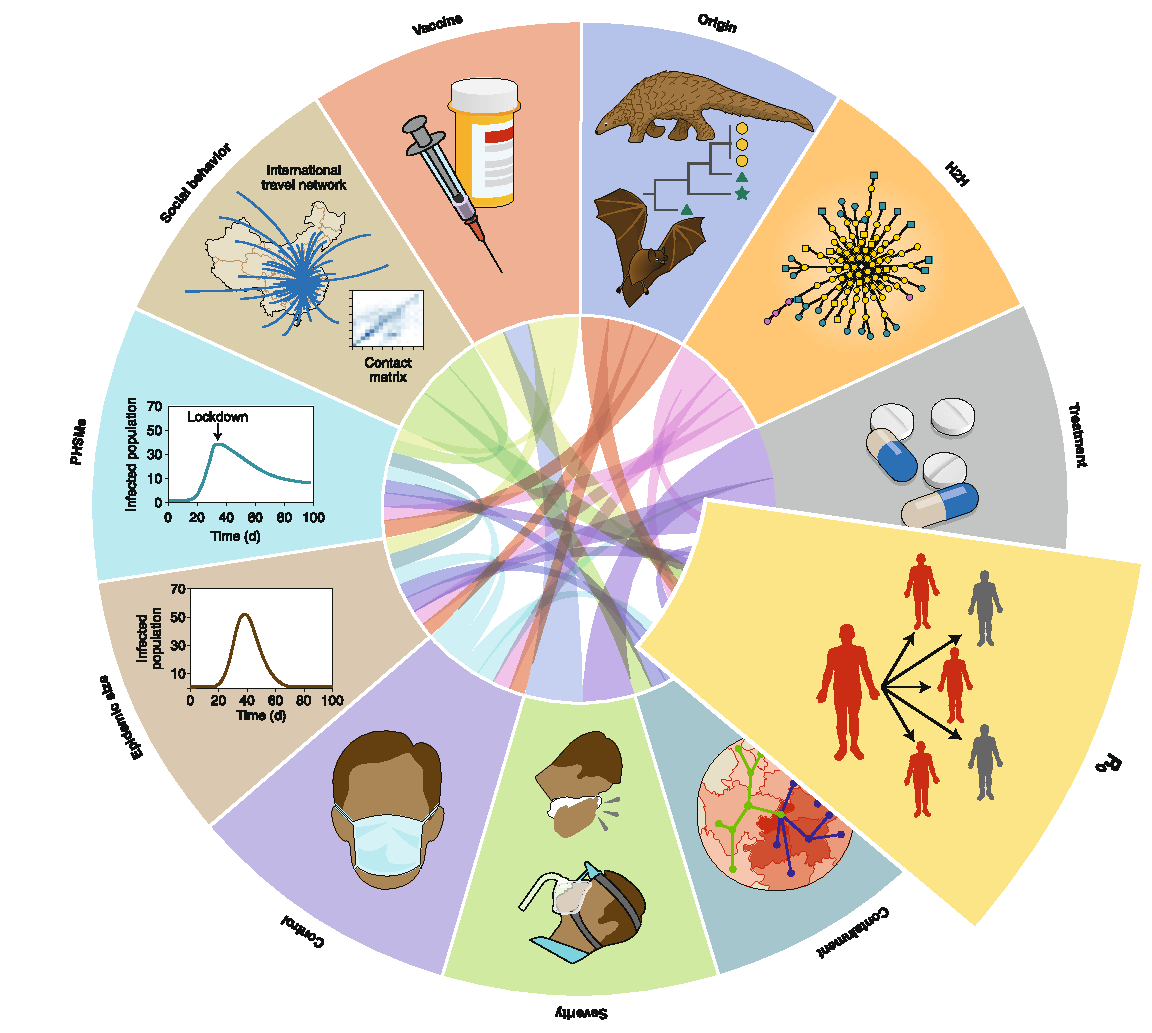
\includegraphics[width=0.9\textwidth]{targets/nowcasting_targets_2.pdf}}%
						\only<3>{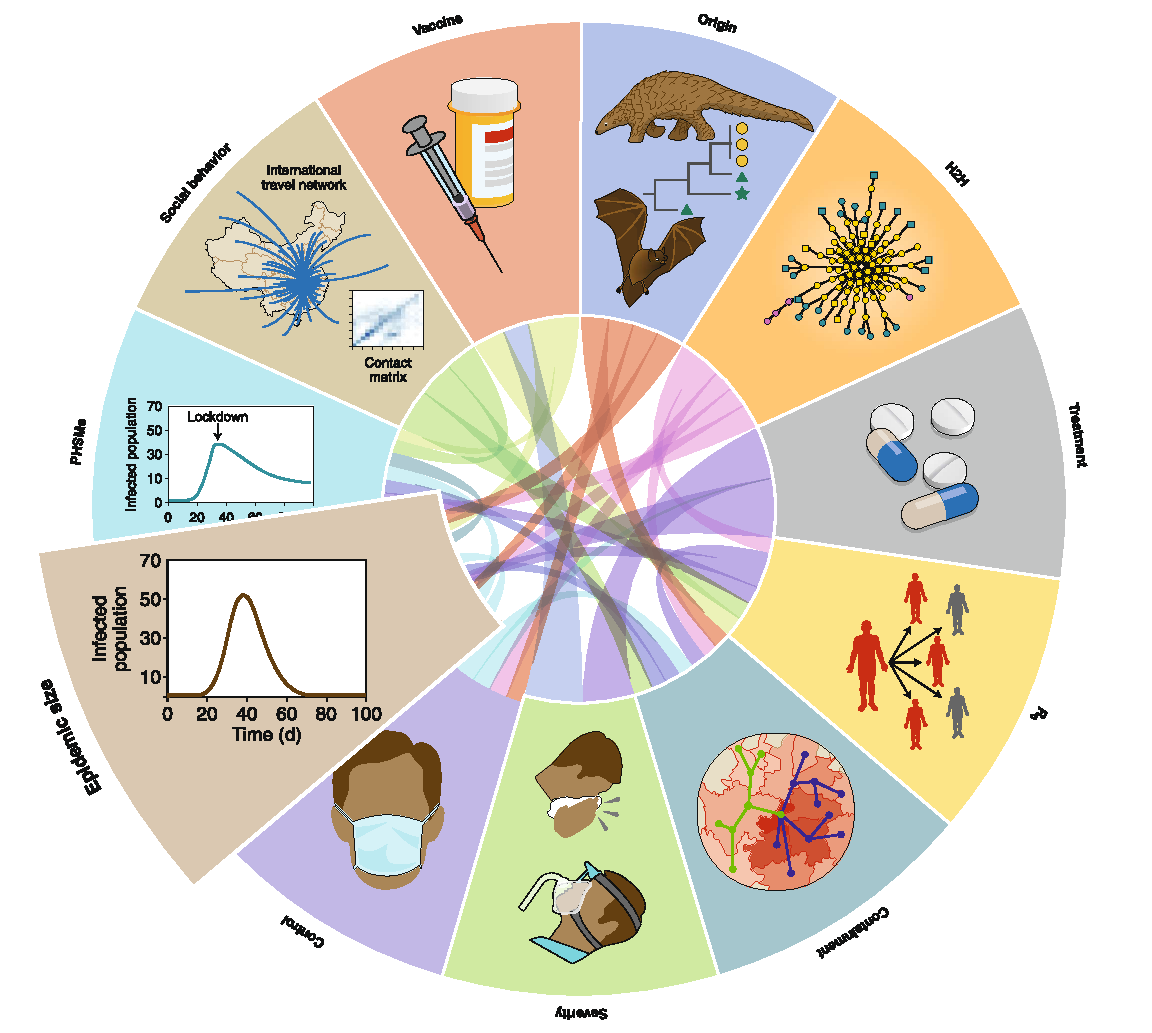
\includegraphics[width=0.9\textwidth]{targets/nowcasting_targets_3.pdf}}%
						\only<4->{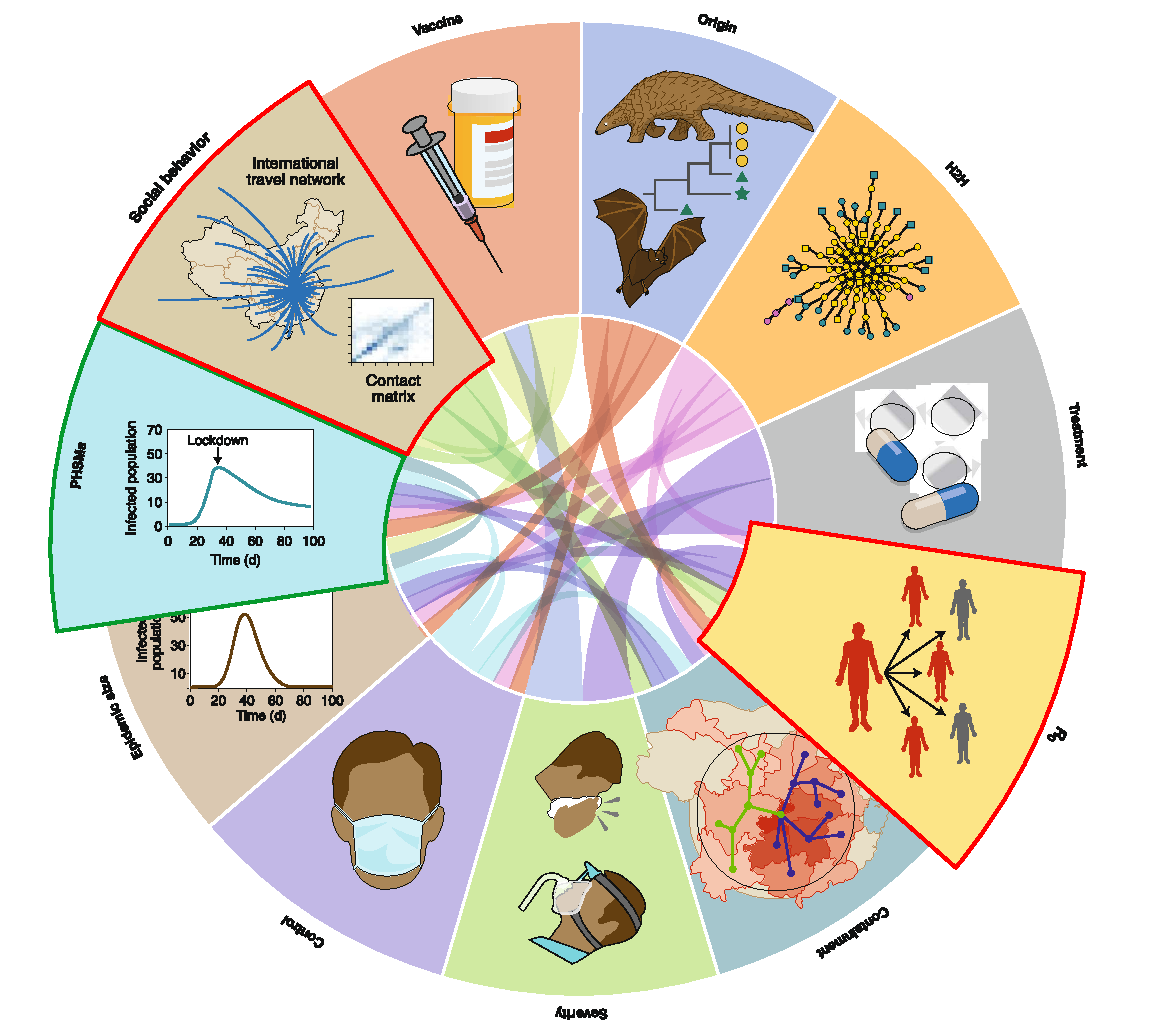
\includegraphics[width=0.9\textwidth]{targets/nowcasting_targets_4.pdf}}%
					};
				% show origin
				% \fill (0,0) circle (2pt);
			\end{tikzpicture}%
		\end{column}
	\end{columns}
	%
	\vspace{-3em}
\end{frame}
\addtocounter{footnote}{-1}
%------------------------------------------------
\begin{frame}[c,noframenumbering]
	\centering
	% \setlength\fboxsep{0pt}
	\begin{titleblock}{}
		\centering 
		~\\%
		{\centering\LARGE Simulation and modeling of pandemics in early stages\ifshowcitations\footnotemark[1]\fi\\}%
		~\\%
		{\textit{Joint work with: Prof. Michael Kokkolaras}}
	\end{titleblock}
	{\color{white}\ifshowcitations\footpartcite{Alhandawi2021b}[1]\fi}
\end{frame}
\addtocounter{footnote}{-1}
%------------------------------------------------

%----------------------------------------------------------------------------------------
%	PRESENTATION SLIDES
%----------------------------------------------------------------------------------------

% \includeonlyframes{abm_2}
% Section 01: background
%------------------------------------------------
\section{Background on epidemiological models}
%------------------------------------------------
\begin{frame}[t,label=abm_1]
	\frametitle{Background: epidemiological models}
	\tikzstyle{background grid}=[draw, black!50,step=.5cm]
	%
	What are compartmental epidemiological models?\\
	%
	\begin{columns}[t] % The "c" option specifies centered vertical alignment while the "t" option is used for top vertical alignment
		\begin{column}{.4\textwidth} % Left column and width
			\small
			\only<-6>{
				\begin{itemize}
					\uncover<2->{\item Described by a \emph{stochastic} process}%
					\uncover<4->{\item Assumes \emph{homogenous} interaction}
					\uncover<5->{\item Deterministic response for large $N$}
				\end{itemize}
				%
				\uncover<6->{
					\begin{equation*}
						\label{eq:SIRodes}
						\begin{aligned}
							&{\frac {dS}{dt}}=-{\frac {\beta IS}{N}},\\[6pt]
							&{\frac {dI}{dt}}={\frac {\beta IS}{N}}-\gamma I,\\[6pt]
							&{\frac {dR}{dt}}=\gamma I,
						\end{aligned}
					\end{equation*}
					{\scriptsize where $N = S + I + R$, $\beta$ controls infection spread, and $\gamma$ controls recovery rate}
				}%
			}%
			\only<7->{
				\begin{itemize}
					\item[\color{darkgreen} \ding{51}]<7-> Analytical solutions are available
					\item[\color{darkgreen} \ding{51}]<8-> Captures large-scale population dynamics
					\item[\color{red} \ding{56}]<9-> Does not account for \emph{geography}
					\item[\color{red} \ding{56}]<10-> Cannot model effect of intervention policies
				\end{itemize}
			}%
			%
		\end{column}
		%
		\begin{column}{.6\textwidth} % Left column and width

			\only<1>{
				\def\framel{1}
				\def\framep{1}
				\def\frameabm{1}
			}%
			\only<2>{
				\def\framel{1}
				\def\framep{2}
				\def\frameabm{1}
			}%
			\only<3>{
				\def\framel{1}
				\def\framep{2}
				\def\frameabm{1}
			}%
			\only<4-8>{
				\def\framel{1}
				\def\framep{2}
				\def\frameabm{2}
			}%
			\only<9->{
				\def\framel{1}
				\def\framep{2}
				\def\frameabm{3}
			}%

			\tikzstyle{background grid}=[draw, black!50,step=.1cm]
			\hspace*{5em}\raisebox{1em}{%
				\begin{tikzpicture}[scale=0.45, every node/.style={scale=0.45}, remember picture, overlay] %show background grid, 
						%%%%%%%%%%%%%%%%%%%%%%%%%%%%%%%%%%%%%%%%%%%%%%%%%%%%%%%%%
% preamble
\newcommand{\scolor}{blue!30}
\newcommand{\icolor}{red!30}
\newcommand{\rcolor}{black!30}
\newcommand{\fcolor}{black!70}
\newcommand{\legendshift}{-3}
%%%%%%%%%%%%%%%%%%%%%%%%%%%%%%%%%%%%%%%%%%%%%%%%%%%%%%%%%
\ifnum \framel = 1
    \renewcommand{\legendshift}{-0}
\else
    \renewcommand{\legendshift}{-3}
\fi
%
\node[circle, minimum size = 10mm, fill=blue!30] (S) at (0+\legendshift,-0) {\Large \color{black} \textit{S}};
\node[circle, minimum size = 10mm, fill=red!30] (I) at (4+\legendshift,-0) {\Large \color{black} \textit{I}};
\node[circle, minimum size = 10mm, fill=black!30] (R) at (8+\legendshift,-0) {\Large \color{black} \textit{R}};
\node[circle, minimum size = 10mm, fill=black!70] (F) at (12+\legendshift,-0) {\Large \color{white} \textit{F}};
%
\node[right, fill=white!70] at (S.east) {\Large susceptible};
\node[right, fill=white!70] at (I.east) {\Large infected};
\node[right, fill=white!70] at (R.east) {\Large recovered};
\node[right, fill=white!70] at (F.east) {\Large fatality};
%
\ifnum \framel > 1
    \node[diamond, minimum size = 12mm, fill=white!70, draw=black, line width=1 pt] (D) at (15+\legendshift,-0) {};
    \node[right, fill=white!70] at (D.east) {\Large random event};
\fi
						%%%%%%%%%%%%%%%%%%%%%%%%%%%%%%%%%%%%%%%%%%%%%%%%%%%%%%%%%
% preamble
\newcommand{\xshiftprocess}{0} 
\newcommand{\yshiftprocess}{-2} 
%%%%%%%%%%%%%%%%%%%%%%%%%%%%%%%%%%%%%%%%%%%%%%%%%%%%%%%%%
\ifnum \framep < 4
    \renewcommand{\yshiftprocess}{-3} 
\else
    \renewcommand{\yshiftprocess}{-2} 
\fi
%
\node[circle, minimum size = 15mm, fill=\scolor] (Ss) at (0+\xshiftprocess,-0+\yshiftprocess) {\LARGE \color{black} \textit{S}};
%
\ifnum \framep > 2
    \node[diamond, aspect=3, fill=white!70, draw=black, line width=1 pt] (contact) at (0+\xshiftprocess,-2.5+\yshiftprocess) {\LARGE made contact?};
    \node[circle, minimum size = 15mm, fill=\icolor] (Is) at (0+\xshiftprocess,-5+\yshiftprocess) {\Large \color{black} \textit{I}};
\else
    \node[circle, minimum size = 15mm, fill=\icolor] (Is) at (0+\xshiftprocess,-4+\yshiftprocess) {\Large \color{black} \textit{I}};
\fi
%
\ifnum \framep > 3
    \node[diamond, aspect=2, fill=white!70, draw=black, line width=1 pt] (hospital) at (0+\xshiftprocess,-7.5+\yshiftprocess) {\LARGE hospitalized?};
    \node[circle, minimum size = 15mm, fill=\rcolor] (Rs) at (-3+\xshiftprocess,-11+\yshiftprocess) {\Large \color{black} \textit{R}};
    \node[circle, minimum size = 15mm, fill=\fcolor] (Fs) at (3+\xshiftprocess,-11+\yshiftprocess) {\Large \color{white} \textit{F}};
\else
    \node[circle, minimum size = 15mm, fill=\rcolor] (Rs) at (-2+\xshiftprocess,-8+\yshiftprocess) {\Large \color{black} \textit{R}};
    \node[circle, minimum size = 15mm, fill=\fcolor] (Fs) at (2+\xshiftprocess,-8+\yshiftprocess) {\Large \color{white} \textit{F}};
\fi
%
\ifnum \framep > 1
    \path[-stealth,every node/.style={inner sep=2pt}]
        \ifnum \framep > 2
            (Ss) edge node [midway] {} (contact)
            (contact) edge node [left=0.1cm] {$P_\mathrm{I}$} (Is)
            {[out=0, in=0, looseness=2, fill=white] (Is) edge node [below=1cm] {$P_\mathrm{reinfect}$} (Ss)}
        \else
            (Ss) edge node [left=0.1cm] {$P_\mathrm{I}$} (Is)
            {[out=0, in=0, looseness=1] (Is) edge node [right=0.1cm] {$P_\mathrm{reinfect}$} (Ss)}
        \fi
        %
        \ifnum \framep > 3
            {[out=270, in=90] (Is.south) edge node {} (hospital.north)}
            %
            {[out=270, in=90] (hospital.south) edge node [below] {$P_{\mathrm{R}|h}$} (Rs.north)}
            {[out=270, in=90] (hospital.south) edge node [below] {$P_{\mathrm{F}|h}$} (Fs)}
            %
            {[out=180, in=90] (hospital.west) edge node [above left] {$P_{\mathrm{R}|h'}$} (Rs.north)}
            {[out=0, in=90] (hospital.east) edge node [above right] {$P_{\mathrm{F}|h'}$} (Fs)}
        \else
            {[out=270, in=90] (Is.south) edge node [above left] {$P_\mathrm{R}$} (Rs.north)}
            {[out=270, in=90] (Is) edge node [midway] [above right] {$P_\mathrm{F}$} (Fs)}
        \fi
    ;
\fi
						\only<3->{%%%%%%%%%%%%%%%%%%%%%%%%%%%%%%%%%%%%%%%%%%%%%%%%%%%%%%%%%
% preamble
\newif\ifS
\newif\ifI
\newif\ifR
\newif\ifF

\newcommand{\infectedlist}{2/4}
\newcommand{\recoveredlist}{2/3,5/5}
\newcommand{\fatalitylist}{3/2,5/1}

\newcommand{\depth}{5} 
\newcommand{\width}{5}  
\newcommand{\spacing}{2.3} 

\newcommand{\xshift}{4} 

\newcommand\IfStringInList[2]{\IfSubStr{,#2,}{,#1,}}

\newcommand{\circlecolor}{\scolor}
%%%%%%%%%%%%%%%%%%%%%%%%%%%%%%%%%%%%%%%%%%%%%%%%%%%%%%%%%
\ifnum \frameabm > 5
    \renewcommand{\recoveredlist}{1/3,2/3,3/3,3/4,3/5,5/5}
\fi

\foreach \i in {1,...,\width}
{
    % Input Layer
    \foreach \j in {1,...,\depth}
    {
        \IfStringInList{\i/\j}{\infectedlist}{\Itrue}{\Ifalse}
        \IfStringInList{\i/\j}{\recoveredlist}{\Rtrue}{\Rfalse}
        \IfStringInList{\i/\j}{\fatalitylist}{\Ftrue}{\Ffalse}
        
        \renewcommand{\circlecolor}{\scolor}
        
        \ifI
            \renewcommand{\circlecolor}{\icolor}
        \fi
        
        \ifR
            \renewcommand{\circlecolor}{\rcolor}
        \fi
        
        \ifF
            \renewcommand{\circlecolor}{\fcolor}
        \fi
            
        \node[circle, 
            minimum size = 10mm,
            fill=\circlecolor] (agent-\i\j) at (\xshift+ \i*\spacing,-\j*\spacing) {};
            
    }
    
}

 % Connect agents
\ifnum \frameabm > 1
    \foreach \i in {1,...,\width}
    {
        \foreach \j in {1,...,\depth}
        {
            \foreach \k in {1,...,\width}
            {
                \foreach \l in {1,...,\depth}
                {
                    
                    \IfSubStr{\i/\j}{\k/\l}{}{
                        
                        % heterogeneous interaction
                        \ifnum \frameabm > 3 
                            \pgfmathsetmacro{\distAB}{sqrt((\i-\k)^2 + (\j-\l)^2)}
                            \ifdim \distAB pt < 1.5 pt
                                
                                \ifnum \frameabm > 4
                                
                                    \IfStringInList{\i/\j}{\infectedlist}{
                                
                                        \IfStringInList{\k/\l}{\recoveredlist}{
                                        
                                            \draw[-, shorten >=1pt, opacity=0.2] (agent-\i\j) -- (agent-\k\l);
                                        }{
                                            \draw[-, color=red, line width=0.45 mm, shorten >=1pt, opacity=1.0] (agent-\i\j) -- (agent-\k\l);
                                        }
                                    }{
                                        \draw[-, shorten >=1pt, opacity=0.2] (agent-\i\j) -- (agent-\k\l);
                                    }
                                \else
                                    \draw[-, shorten >=1pt, opacity=0.4] (agent-\i\j) -- (agent-\k\l);
                                \fi
                                
                        \fi
                        \else
                            % homogeneous interaction
                            \IfStringInList{\i/\j}{\infectedlist}{
                                \ifnum \frameabm > 2
                                    \IfStringInList{\k/\l}{\recoveredlist}{
                                        \draw[-, shorten >=1pt, opacity=0.1] (agent-\i\j) -- (agent-\k\l);
                                    }{
                                        \draw[-, color=red, line width=0.45 mm, shorten >=1pt, opacity=1.0] (agent-\i\j) -- (agent-\k\l);
                                    }
                                \else
                                    \draw[-, shorten >=1pt, opacity=0.1] (agent-\i\j) -- (agent-\k\l);
                                \fi
                            }{
                                \draw[-, shorten >=1pt, opacity=0.1] (agent-\i\j) -- (agent-\k\l);
                            }
                        \fi
                    }
                }
            }
        }
    }
\fi}
				\end{tikzpicture}%
			}%
			\begin{tikzpicture}[remember picture, overlay] %show background grid, 
				\node [inner sep=0pt,above right, opacity=1.0]  at (-0.13\textwidth,-0.66\textheight) (seir) 
					{
						\only<6>{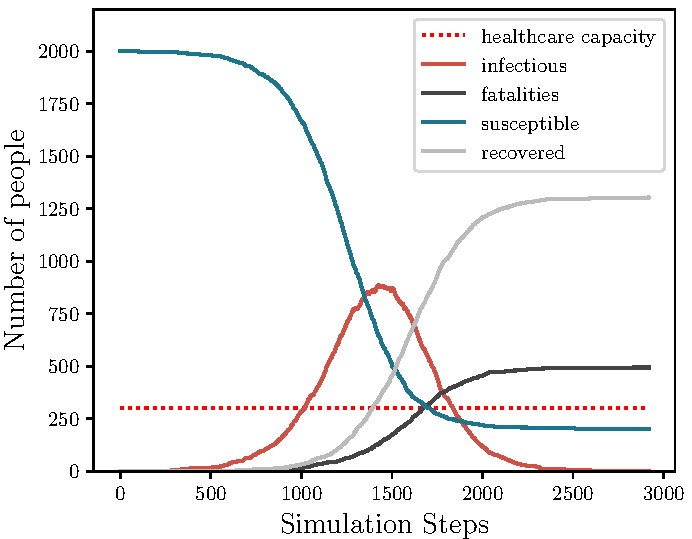
\includegraphics[width=0.9\textwidth]{SIR_example.pdf}}%
					};
			\end{tikzpicture}%
		\end{column}

	\end{columns}
	\vspace{-3em}
\end{frame}
%------------------------------------------------
\begin{frame}[t,label=abm_2]
	\frametitle{Background: epidemiological models}
	\tikzstyle{background grid}=[draw, black!50,step=.5cm]
	%
	What are agent-based epidemiological models?\\
	%
	\begin{columns}[t] % The "c" option specifies centered vertical alignment while the "t" option is used for top vertical alignment
		\begin{column}{.4\textwidth} % Left column and width
			\small
			\only<-12>{
				\begin{itemize}
					\uncover<2->{\item \emph{Stochastic} process}%
					\uncover<3->{\item Assume \emph{heterogenous} interaction}
					\uncover<5-12>{\item Stochastic response}
				\end{itemize}
			}%
			\only<13->{
				\begin{itemize}
					\item[\color{darkgreen} \ding{51}]<13-> Account for \emph{geography} and \emph{demographics}
					\item[\color{darkgreen} \ding{51}]<14-> Describe local phenomena
					\item[\color{darkgreen} \ding{51}]<15-> Can be used to model intervention policies
					\item[\color{red} \ding{56}]<16-> Stochastic response makes decision making challenging
					\item[\color{red} \ding{56}]<17-> Computationally expensive
				\end{itemize}
			}%
			%
		\end{column}
		%
		\begin{column}{.6\textwidth} % Left column and width

			\only<1>{
				\def\framel{1}
				\def\framep{2}
				\def\frameabm{1}
			}%
			\only<2>{
				\def\framel{2}
				\def\framep{3}
				\def\frameabm{1}
			}%
			\only<3>{
				\def\framel{2}
				\def\framep{3}
				\def\frameabm{4}
			}%
			\only<4-14>{
				\def\framel{2}
				\def\framep{3}
				\def\frameabm{5}
			}%
			\only<15->{
				\def\framel{2}
				\def\framep{4}
				\def\frameabm{6}
			}%
			\tikzstyle{background grid}=[draw, black!50,step=.1cm]
			\only<-4,13->{
				\hspace*{5em}\raisebox{1em}{%
					\begin{tikzpicture}[scale=0.45, every node/.style={scale=0.45}, remember picture, overlay] %show background grid, 
							%%%%%%%%%%%%%%%%%%%%%%%%%%%%%%%%%%%%%%%%%%%%%%%%%%%%%%%%%
% preamble
\newcommand{\scolor}{blue!30}
\newcommand{\icolor}{red!30}
\newcommand{\rcolor}{black!30}
\newcommand{\fcolor}{black!70}
\newcommand{\legendshift}{-3}
%%%%%%%%%%%%%%%%%%%%%%%%%%%%%%%%%%%%%%%%%%%%%%%%%%%%%%%%%
\ifnum \framel = 1
    \renewcommand{\legendshift}{-0}
\else
    \renewcommand{\legendshift}{-3}
\fi
%
\node[circle, minimum size = 10mm, fill=blue!30] (S) at (0+\legendshift,-0) {\Large \color{black} \textit{S}};
\node[circle, minimum size = 10mm, fill=red!30] (I) at (4+\legendshift,-0) {\Large \color{black} \textit{I}};
\node[circle, minimum size = 10mm, fill=black!30] (R) at (8+\legendshift,-0) {\Large \color{black} \textit{R}};
\node[circle, minimum size = 10mm, fill=black!70] (F) at (12+\legendshift,-0) {\Large \color{white} \textit{F}};
%
\node[right, fill=white!70] at (S.east) {\Large susceptible};
\node[right, fill=white!70] at (I.east) {\Large infected};
\node[right, fill=white!70] at (R.east) {\Large recovered};
\node[right, fill=white!70] at (F.east) {\Large fatality};
%
\ifnum \framel > 1
    \node[diamond, minimum size = 12mm, fill=white!70, draw=black, line width=1 pt] (D) at (15+\legendshift,-0) {};
    \node[right, fill=white!70] at (D.east) {\Large random event};
\fi
							%%%%%%%%%%%%%%%%%%%%%%%%%%%%%%%%%%%%%%%%%%%%%%%%%%%%%%%%%
% preamble
\newcommand{\xshiftprocess}{0} 
\newcommand{\yshiftprocess}{-2} 
%%%%%%%%%%%%%%%%%%%%%%%%%%%%%%%%%%%%%%%%%%%%%%%%%%%%%%%%%
\ifnum \framep < 4
    \renewcommand{\yshiftprocess}{-3} 
\else
    \renewcommand{\yshiftprocess}{-2} 
\fi
%
\node[circle, minimum size = 15mm, fill=\scolor] (Ss) at (0+\xshiftprocess,-0+\yshiftprocess) {\LARGE \color{black} \textit{S}};
%
\ifnum \framep > 2
    \node[diamond, aspect=3, fill=white!70, draw=black, line width=1 pt] (contact) at (0+\xshiftprocess,-2.5+\yshiftprocess) {\LARGE made contact?};
    \node[circle, minimum size = 15mm, fill=\icolor] (Is) at (0+\xshiftprocess,-5+\yshiftprocess) {\Large \color{black} \textit{I}};
\else
    \node[circle, minimum size = 15mm, fill=\icolor] (Is) at (0+\xshiftprocess,-4+\yshiftprocess) {\Large \color{black} \textit{I}};
\fi
%
\ifnum \framep > 3
    \node[diamond, aspect=2, fill=white!70, draw=black, line width=1 pt] (hospital) at (0+\xshiftprocess,-7.5+\yshiftprocess) {\LARGE hospitalized?};
    \node[circle, minimum size = 15mm, fill=\rcolor] (Rs) at (-3+\xshiftprocess,-11+\yshiftprocess) {\Large \color{black} \textit{R}};
    \node[circle, minimum size = 15mm, fill=\fcolor] (Fs) at (3+\xshiftprocess,-11+\yshiftprocess) {\Large \color{white} \textit{F}};
\else
    \node[circle, minimum size = 15mm, fill=\rcolor] (Rs) at (-2+\xshiftprocess,-8+\yshiftprocess) {\Large \color{black} \textit{R}};
    \node[circle, minimum size = 15mm, fill=\fcolor] (Fs) at (2+\xshiftprocess,-8+\yshiftprocess) {\Large \color{white} \textit{F}};
\fi
%
\ifnum \framep > 1
    \path[-stealth,every node/.style={inner sep=2pt}]
        \ifnum \framep > 2
            (Ss) edge node [midway] {} (contact)
            (contact) edge node [left=0.1cm] {$P_\mathrm{I}$} (Is)
            {[out=0, in=0, looseness=2, fill=white] (Is) edge node [below=1cm] {$P_\mathrm{reinfect}$} (Ss)}
        \else
            (Ss) edge node [left=0.1cm] {$P_\mathrm{I}$} (Is)
            {[out=0, in=0, looseness=1] (Is) edge node [right=0.1cm] {$P_\mathrm{reinfect}$} (Ss)}
        \fi
        %
        \ifnum \framep > 3
            {[out=270, in=90] (Is.south) edge node {} (hospital.north)}
            %
            {[out=270, in=90] (hospital.south) edge node [below] {$P_{\mathrm{R}|h}$} (Rs.north)}
            {[out=270, in=90] (hospital.south) edge node [below] {$P_{\mathrm{F}|h}$} (Fs)}
            %
            {[out=180, in=90] (hospital.west) edge node [above left] {$P_{\mathrm{R}|h'}$} (Rs.north)}
            {[out=0, in=90] (hospital.east) edge node [above right] {$P_{\mathrm{F}|h'}$} (Fs)}
        \else
            {[out=270, in=90] (Is.south) edge node [above left] {$P_\mathrm{R}$} (Rs.north)}
            {[out=270, in=90] (Is) edge node [midway] [above right] {$P_\mathrm{F}$} (Fs)}
        \fi
    ;
\fi
							%%%%%%%%%%%%%%%%%%%%%%%%%%%%%%%%%%%%%%%%%%%%%%%%%%%%%%%%%
% preamble
\newif\ifS
\newif\ifI
\newif\ifR
\newif\ifF

\newcommand{\infectedlist}{2/4}
\newcommand{\recoveredlist}{2/3,5/5}
\newcommand{\fatalitylist}{3/2,5/1}

\newcommand{\depth}{5} 
\newcommand{\width}{5}  
\newcommand{\spacing}{2.3} 

\newcommand{\xshift}{4} 

\newcommand\IfStringInList[2]{\IfSubStr{,#2,}{,#1,}}

\newcommand{\circlecolor}{\scolor}
%%%%%%%%%%%%%%%%%%%%%%%%%%%%%%%%%%%%%%%%%%%%%%%%%%%%%%%%%
\ifnum \frameabm > 5
    \renewcommand{\recoveredlist}{1/3,2/3,3/3,3/4,3/5,5/5}
\fi

\foreach \i in {1,...,\width}
{
    % Input Layer
    \foreach \j in {1,...,\depth}
    {
        \IfStringInList{\i/\j}{\infectedlist}{\Itrue}{\Ifalse}
        \IfStringInList{\i/\j}{\recoveredlist}{\Rtrue}{\Rfalse}
        \IfStringInList{\i/\j}{\fatalitylist}{\Ftrue}{\Ffalse}
        
        \renewcommand{\circlecolor}{\scolor}
        
        \ifI
            \renewcommand{\circlecolor}{\icolor}
        \fi
        
        \ifR
            \renewcommand{\circlecolor}{\rcolor}
        \fi
        
        \ifF
            \renewcommand{\circlecolor}{\fcolor}
        \fi
            
        \node[circle, 
            minimum size = 10mm,
            fill=\circlecolor] (agent-\i\j) at (\xshift+ \i*\spacing,-\j*\spacing) {};
            
    }
    
}

 % Connect agents
\ifnum \frameabm > 1
    \foreach \i in {1,...,\width}
    {
        \foreach \j in {1,...,\depth}
        {
            \foreach \k in {1,...,\width}
            {
                \foreach \l in {1,...,\depth}
                {
                    
                    \IfSubStr{\i/\j}{\k/\l}{}{
                        
                        % heterogeneous interaction
                        \ifnum \frameabm > 3 
                            \pgfmathsetmacro{\distAB}{sqrt((\i-\k)^2 + (\j-\l)^2)}
                            \ifdim \distAB pt < 1.5 pt
                                
                                \ifnum \frameabm > 4
                                
                                    \IfStringInList{\i/\j}{\infectedlist}{
                                
                                        \IfStringInList{\k/\l}{\recoveredlist}{
                                        
                                            \draw[-, shorten >=1pt, opacity=0.2] (agent-\i\j) -- (agent-\k\l);
                                        }{
                                            \draw[-, color=red, line width=0.45 mm, shorten >=1pt, opacity=1.0] (agent-\i\j) -- (agent-\k\l);
                                        }
                                    }{
                                        \draw[-, shorten >=1pt, opacity=0.2] (agent-\i\j) -- (agent-\k\l);
                                    }
                                \else
                                    \draw[-, shorten >=1pt, opacity=0.4] (agent-\i\j) -- (agent-\k\l);
                                \fi
                                
                        \fi
                        \else
                            % homogeneous interaction
                            \IfStringInList{\i/\j}{\infectedlist}{
                                \ifnum \frameabm > 2
                                    \IfStringInList{\k/\l}{\recoveredlist}{
                                        \draw[-, shorten >=1pt, opacity=0.1] (agent-\i\j) -- (agent-\k\l);
                                    }{
                                        \draw[-, color=red, line width=0.45 mm, shorten >=1pt, opacity=1.0] (agent-\i\j) -- (agent-\k\l);
                                    }
                                \else
                                    \draw[-, shorten >=1pt, opacity=0.1] (agent-\i\j) -- (agent-\k\l);
                                \fi
                            }{
                                \draw[-, shorten >=1pt, opacity=0.1] (agent-\i\j) -- (agent-\k\l);
                            }
                        \fi
                    }
                }
            }
        }
    }
\fi
					\end{tikzpicture}%
				}%
			}%
			%
			\begin{tikzpicture}[remember picture, overlay] %show background grid, 
				\node [inner sep=0pt,above right, opacity=1.0]  at (0.1\textwidth,-0.66\textheight) (abm) 
					{
						\only<5>{
							\begin{animateinline}[autoplay,width=0.9\textwidth]{60}
								\ifshowanimations
									\multiframe{77}{i=5+45}{%
										\includegraphics{render_demo_1_realization_1/sim_\i.pdf}
									}
								\else
									\multiframe{1}{i=3500+0}{%
										\includegraphics{render_demo_1_realization_1/sim_\i.pdf}
									}
								\fi
							\end{animateinline}%
						}%
						\only<6>{
							\begin{animateinline}[autoplay,width=0.9\textwidth]{60}
								\ifshowanimations
									\multiframe{77}{i=5+45}{%
										\includegraphics{render_demo_1_realization_2/sim_\i.pdf}
									}
								\else
									\multiframe{1}{i=3500+0}{%
										\includegraphics{render_demo_1_realization_2/sim_\i.pdf}
									}
								\fi
							\end{animateinline}%
						}%
					};
				\only<5>{\node[inner sep=0pt,align=flush center,above=\belowcaptionskip of abm,text width=\linewidth]
					{\vspace{-1em}{\large Realization 1}};}%
				\only<6>{\node[inner sep=0pt,align=flush center,above=\belowcaptionskip of abm,text width=\linewidth]
					{\vspace{-1em}{\large Realization 2}};}%
				%
				\node [inner sep=0pt,above right, opacity=1.0]  at (0.1\textwidth,-0.69\textheight) (trajectory) 
				{
					\only<7>{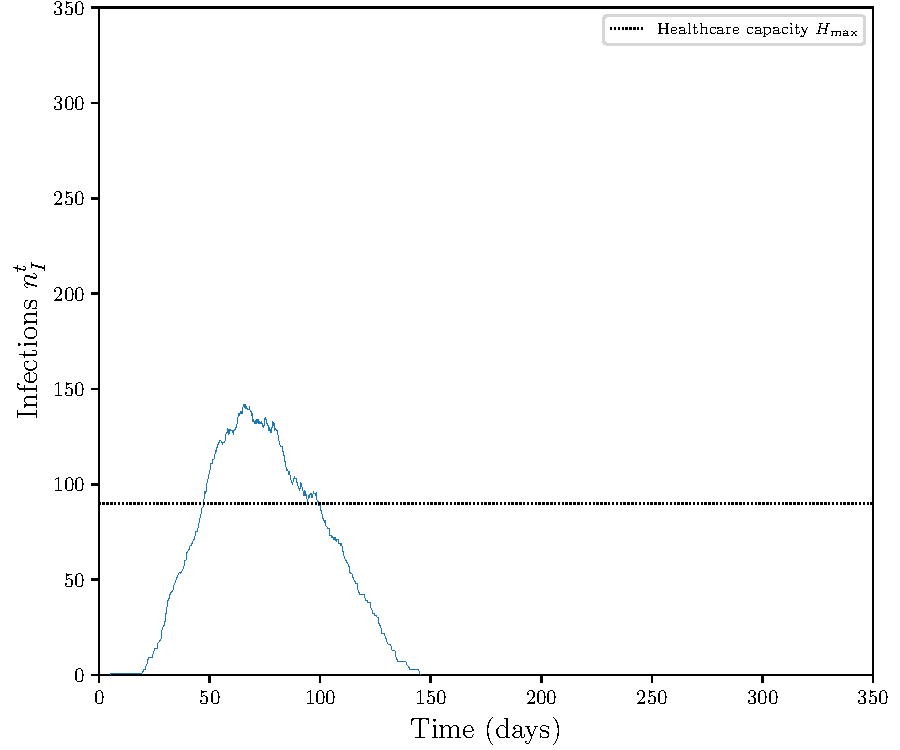
\includegraphics[width=0.85\textwidth]{realization_traces/I_compare_R_0.pdf}}%
					\only<8>{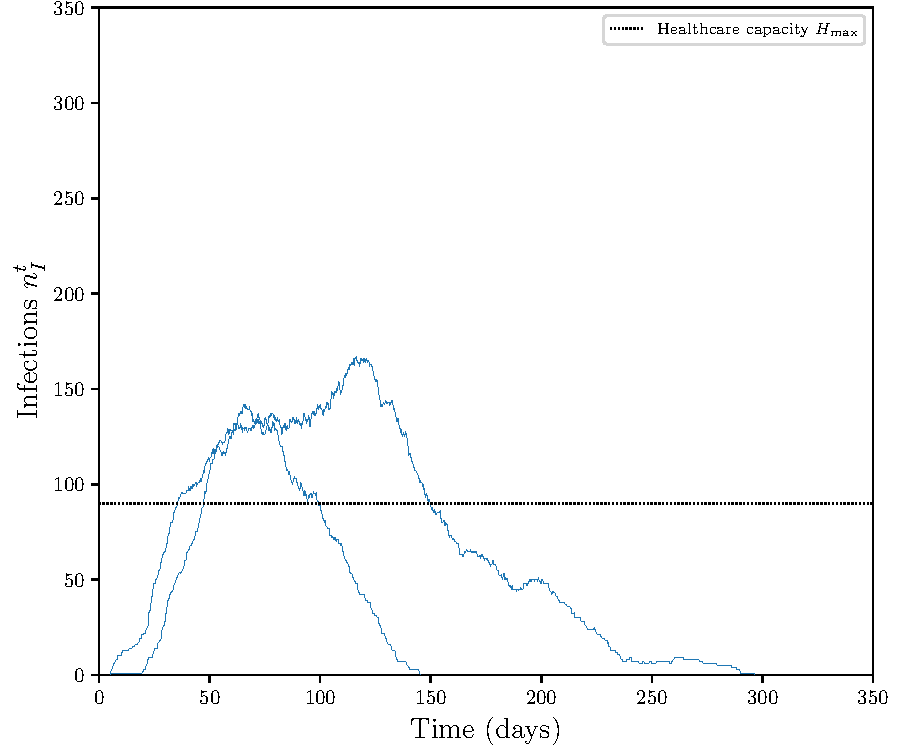
\includegraphics[width=0.85\textwidth]{realization_traces/I_compare_R_1.pdf}}%
					\only<9>{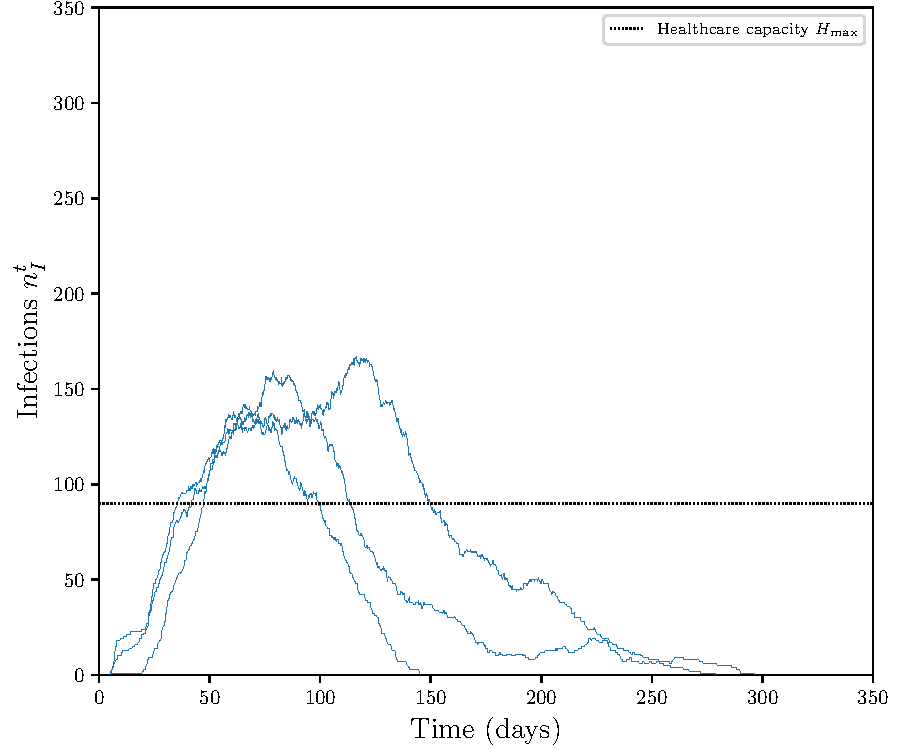
\includegraphics[width=0.85\textwidth]{realization_traces/I_compare_R_2.pdf}}%
					\only<10>{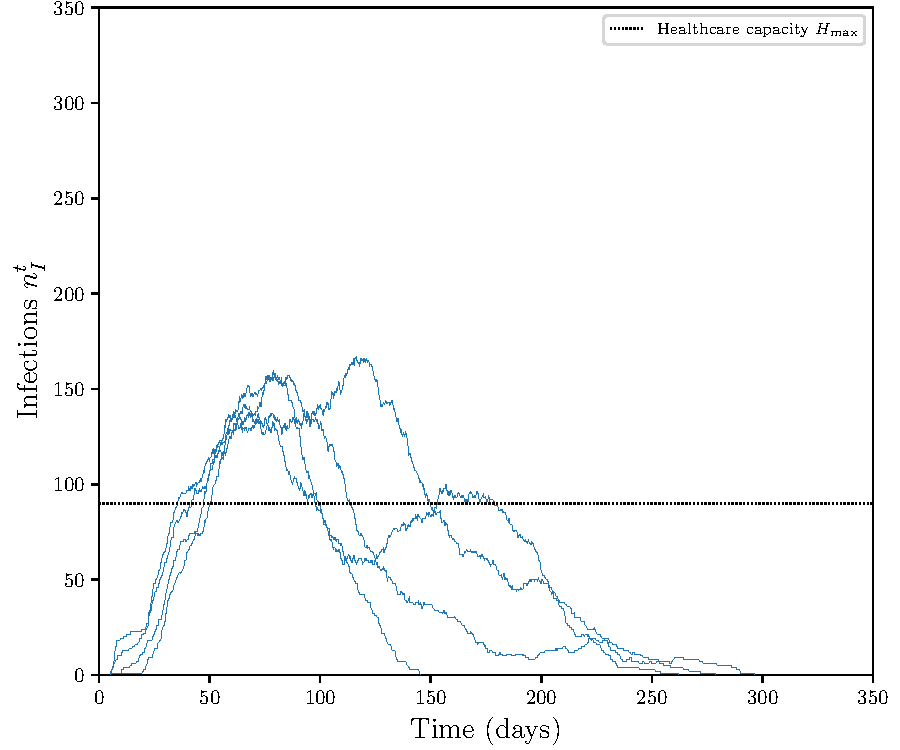
\includegraphics[width=0.85\textwidth]{realization_traces/I_compare_R_3.pdf}}%
					\only<11>{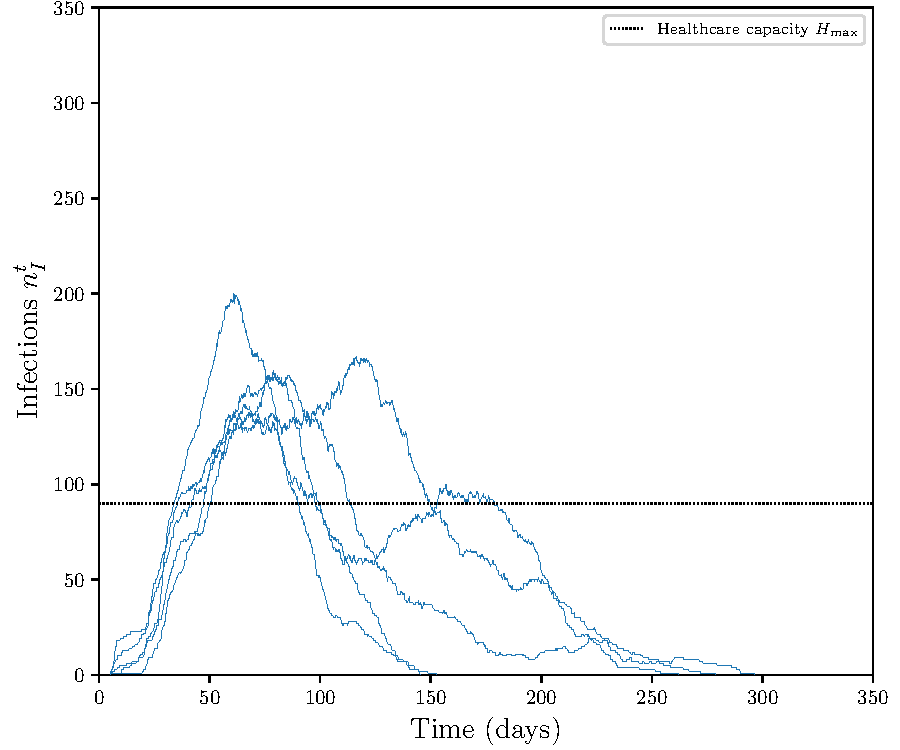
\includegraphics[width=0.85\textwidth]{realization_traces/I_compare_R_4.pdf}}%
					\only<12>{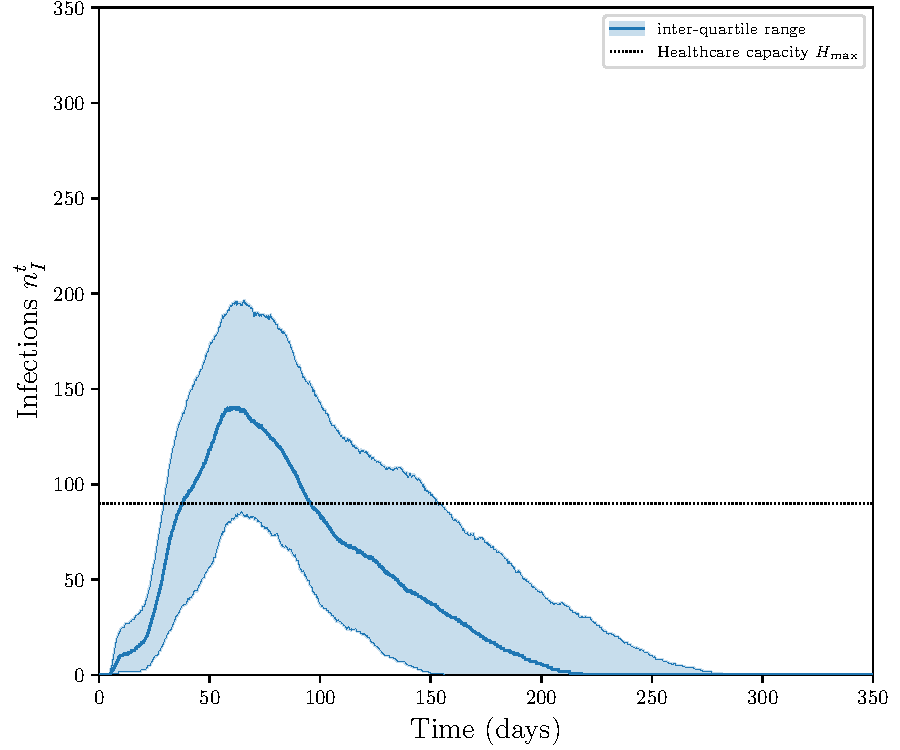
\includegraphics[width=0.85\textwidth]{realization_traces/I_compare_opt_0.pdf}}%
				};
				\only<7>{\node[inner sep=0pt,align=flush center,above=\belowcaptionskip of trajectory,text width=\linewidth]
					{\vspace{-1em}{\large Realization 1}};}%
				\only<8>{\node[inner sep=0pt,align=flush center,above=\belowcaptionskip of trajectory,text width=\linewidth]
					{\vspace{-1em}{\large Realization 2}};}%
			\end{tikzpicture}%
		\end{column}

	\end{columns}
	\vspace{-3em}
\end{frame}

% Section 02: problem formulation
%------------------------------------------------
\section{Public health policy-making problem}
%------------------------------------------------
\begin{frame}[t,label=abm_3]
	\frametitle{Public health policy-making problem formulation}
	\tikzstyle{background grid}=[draw, black!50,step=.5cm]
	%
	What is the \emphasis{cost} of public health interventions?\\
	%
	\begin{columns}[t] % The "c" option specifies centered vertical alignment while the "t" option is used for top vertical alignment
		\begin{column}{.5\textwidth} % Left column and width

			\begin{tikzpicture}[remember picture, overlay] %show background grid, 
				\node [inner sep=0pt,above right, opacity=1.0]  at (0.0\textwidth,-0.66\textheight) (abm) 
					{
						\only<-5>{
							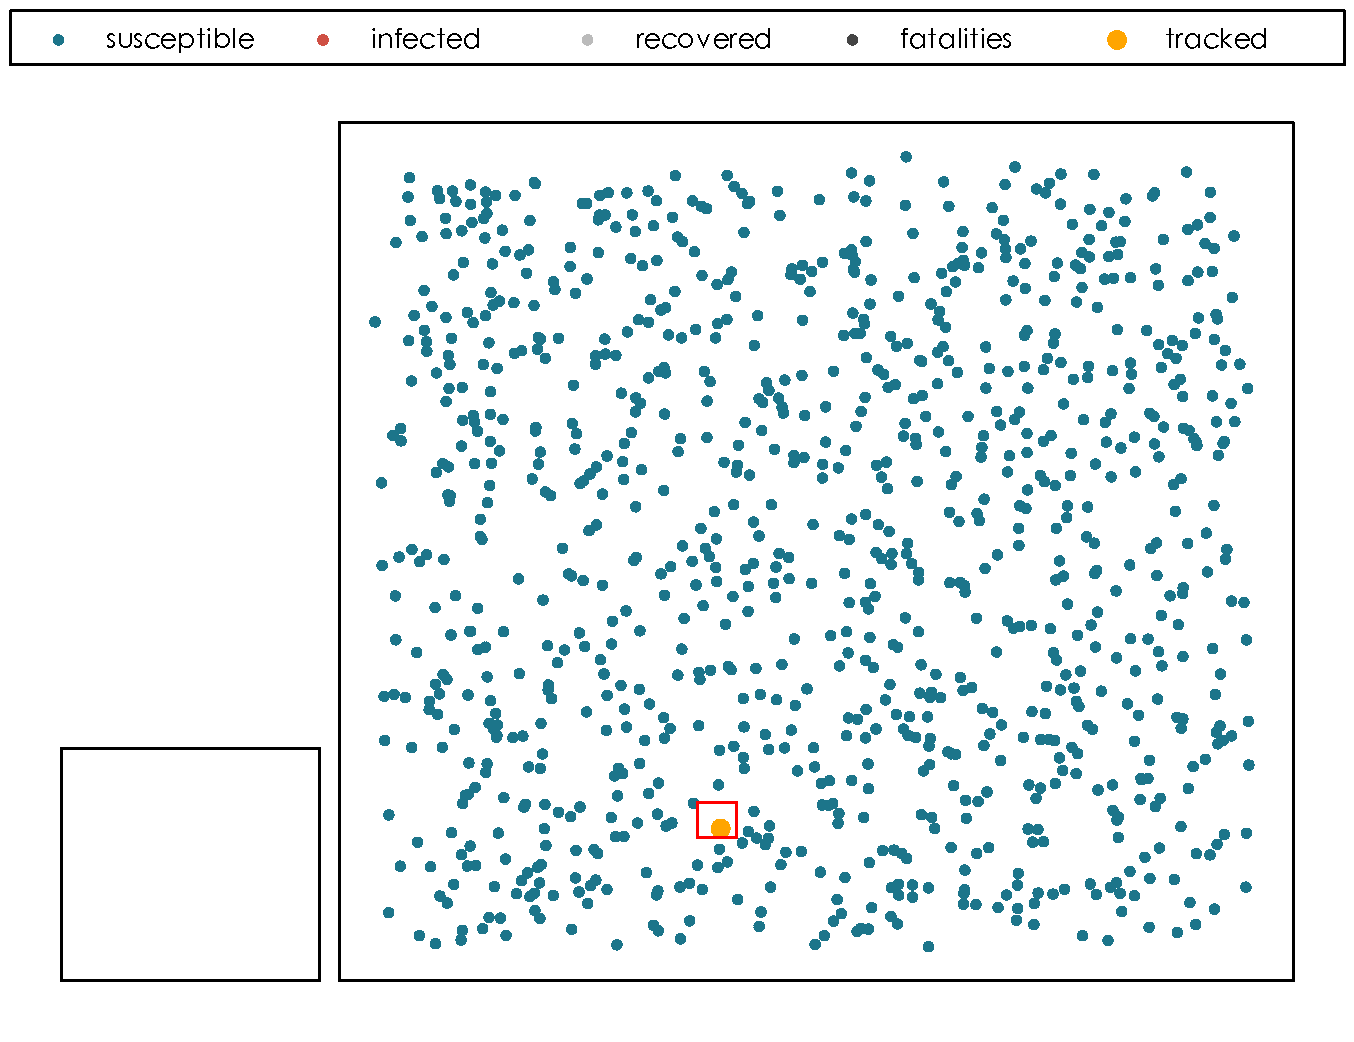
\includegraphics[width=0.95\textwidth]{render_2_no_restrictions/sim_10.pdf}
						}%	
						\only<6>{
							\begin{animateinline}[autoplay,width=0.95\textwidth]{70}
								\ifshowanimations
									\multiframe{77}{i=10+45}{%
										\includegraphics{render_2_no_restrictions/sim_\i.pdf}
									}
								\else
									\multiframe{1}{i=10+0}{%
										\includegraphics{render_2_no_restrictions/sim_\i.pdf}
									}
								\fi
							\end{animateinline}%
						}%
						\only<7>{
							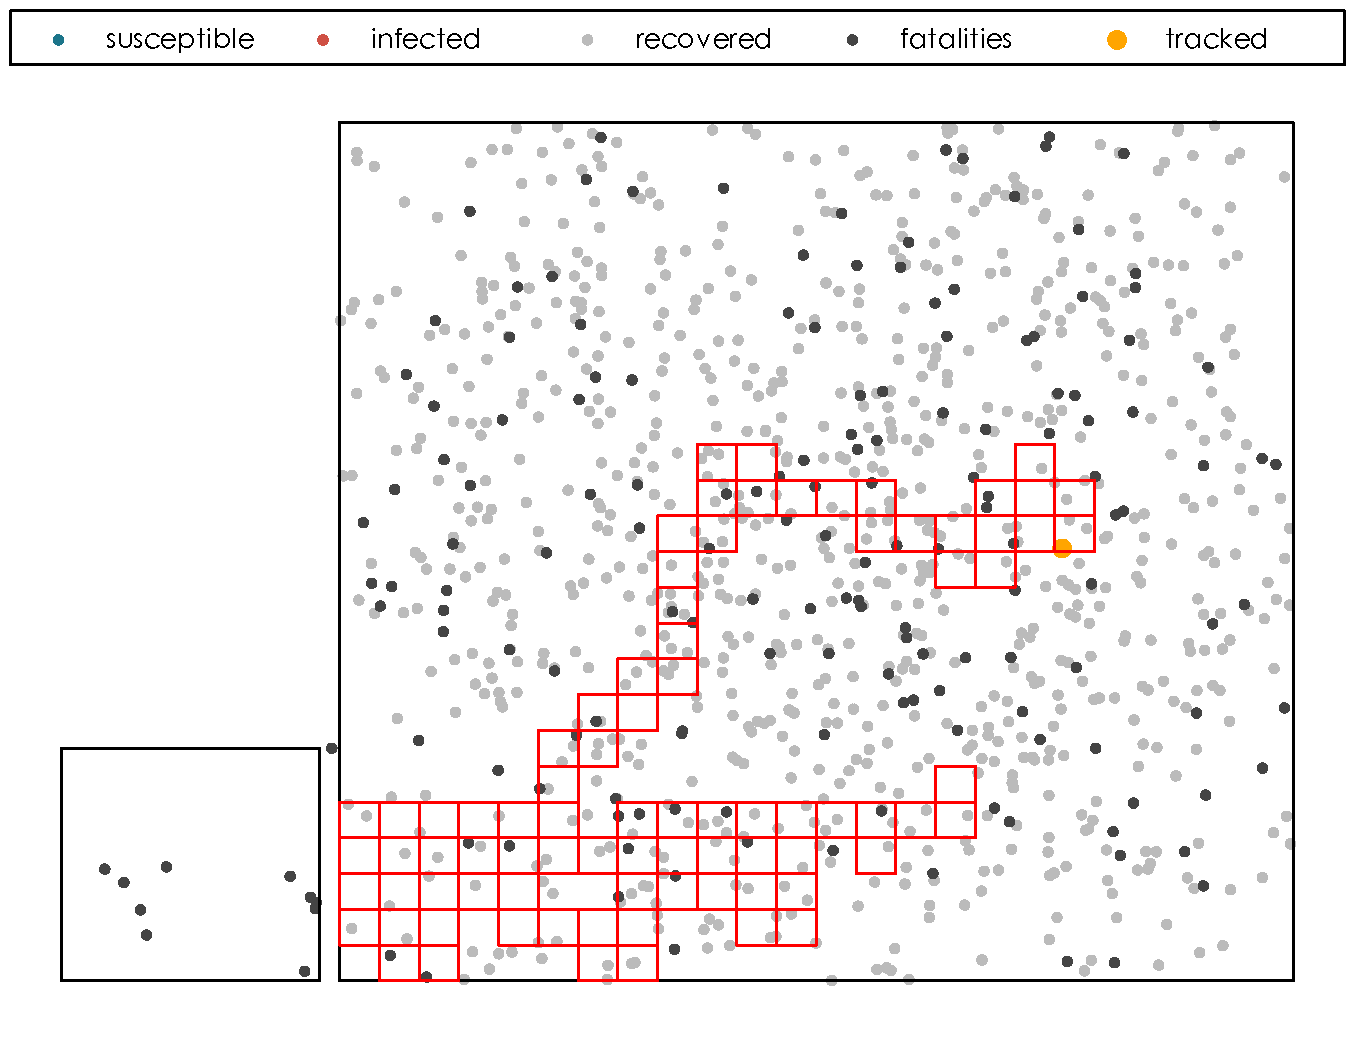
\includegraphics[width=0.95\textwidth]{render_2_no_restrictions/sim_3500.pdf}
						}%
					};
				\only<1-7>{\node[inner sep=0pt,align=flush center,above=\belowcaptionskip of abm,text width=\linewidth]
					{\vspace{-1em}{\large No interventions applied}};}%
				%
				\node [inner sep=0pt,above right, opacity=1.0]  at (0.0\textwidth,-0.69\textheight) (infection) 
				{
					\only<8>{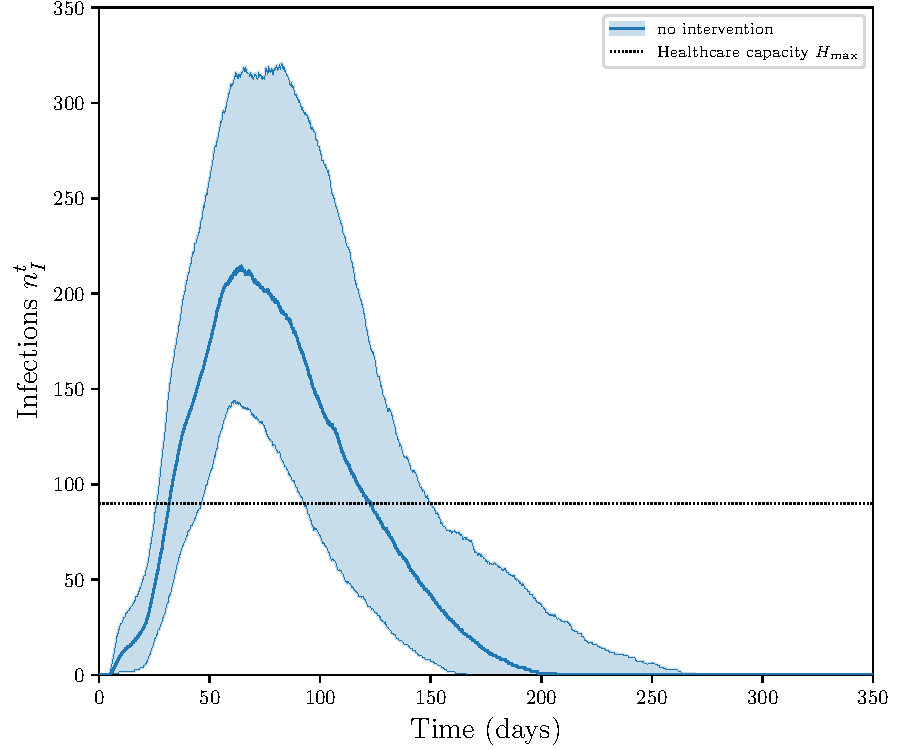
\includegraphics[width=0.9\textwidth]{trajectory_demo/I_compare_opt_1.pdf}}%
					\only<9>{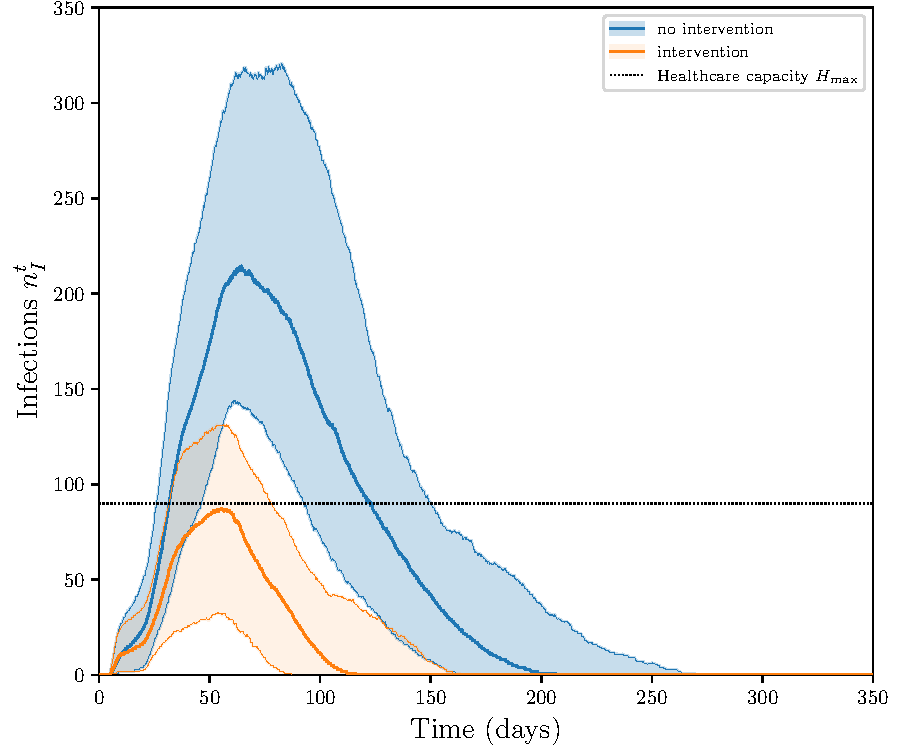
\includegraphics[width=0.9\textwidth]{trajectory_demo/I_compare_opt_3.pdf}}%
				};

				\only<9>{
					\node[inner sep=0pt,align=flush center,above=\belowcaptionskip of infection,text width=\linewidth]
					{\vspace{-1em}{
						\large {\color{darkgreen} infections $\downarrow$}
					}};
				}%

			\end{tikzpicture}%

		\end{column}
		%
		\begin{column}{.5\textwidth} % Left column and width

			\tikzstyle{background grid}=[draw, black!50,step=.1cm]
			\begin{tikzpicture}[remember picture, overlay] %show background grid, 
				\node [inner sep=0pt,above right, opacity=1.0]  at (0.0\textwidth,-0.66\textheight) (abm) 
					{
						\only<2-5>{
							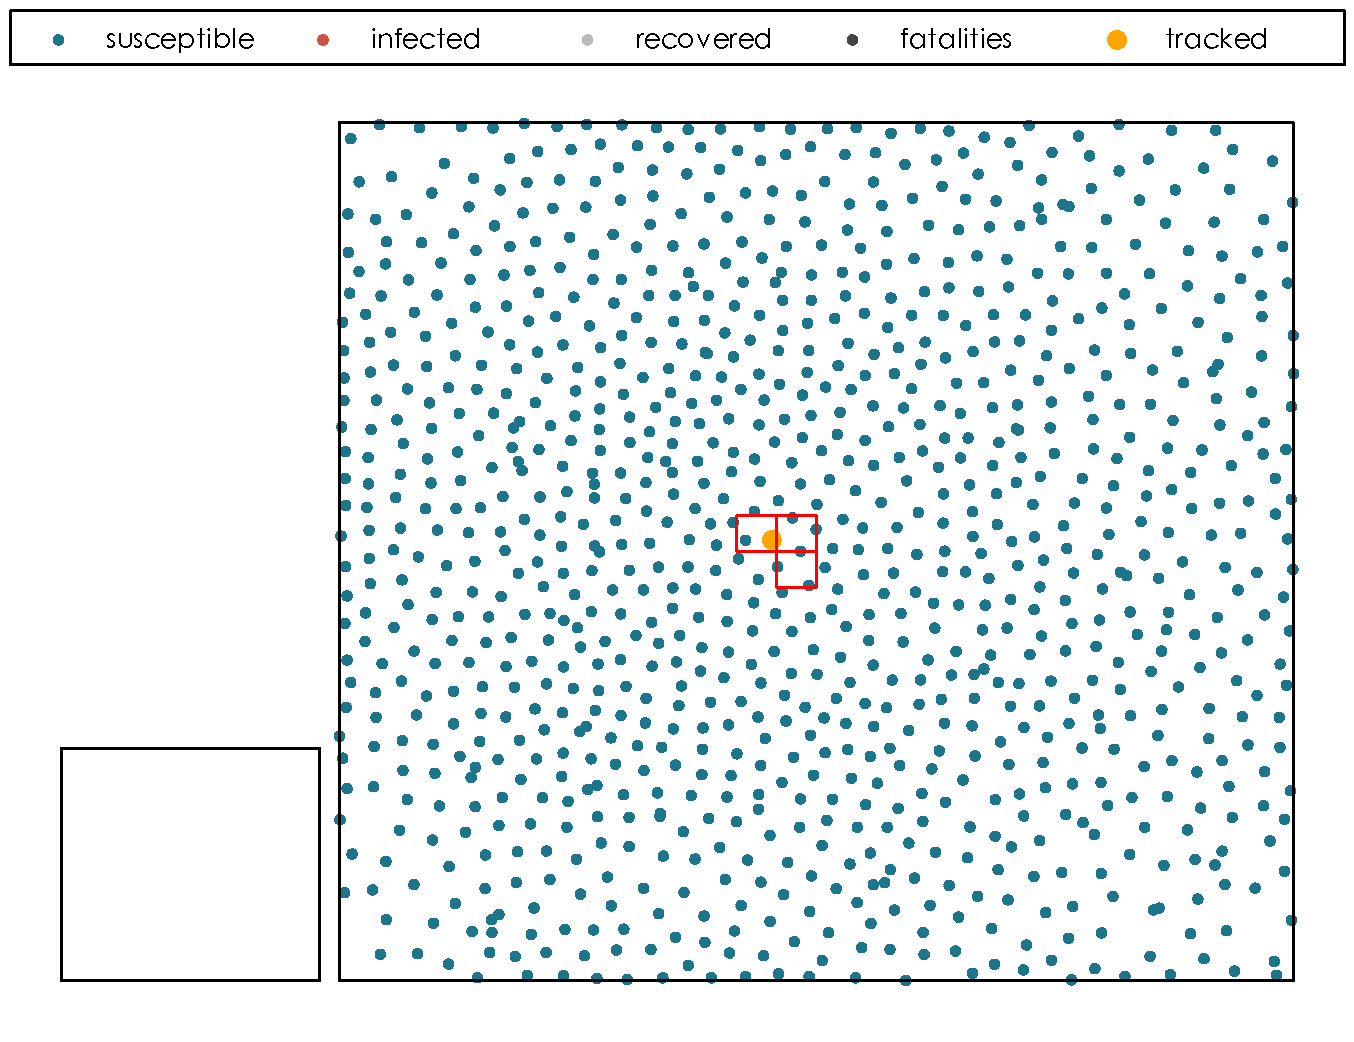
\includegraphics[width=0.95\textwidth]{render_1_restrictions/sim_50.pdf}
						}%	
						\only<6>{
							\begin{animateinline}[autoplay,width=0.95\textwidth]{70}
								\ifshowanimations
									\multiframe{75}{i=50+45}{%
										\includegraphics{render_1_restrictions/sim_\i.pdf}
									}
								\else
									\multiframe{1}{i=50+0}{%
										\includegraphics{render_1_restrictions/sim_\i.pdf}
									}
								\fi
							\end{animateinline}%
						}%
						\only<7>{
							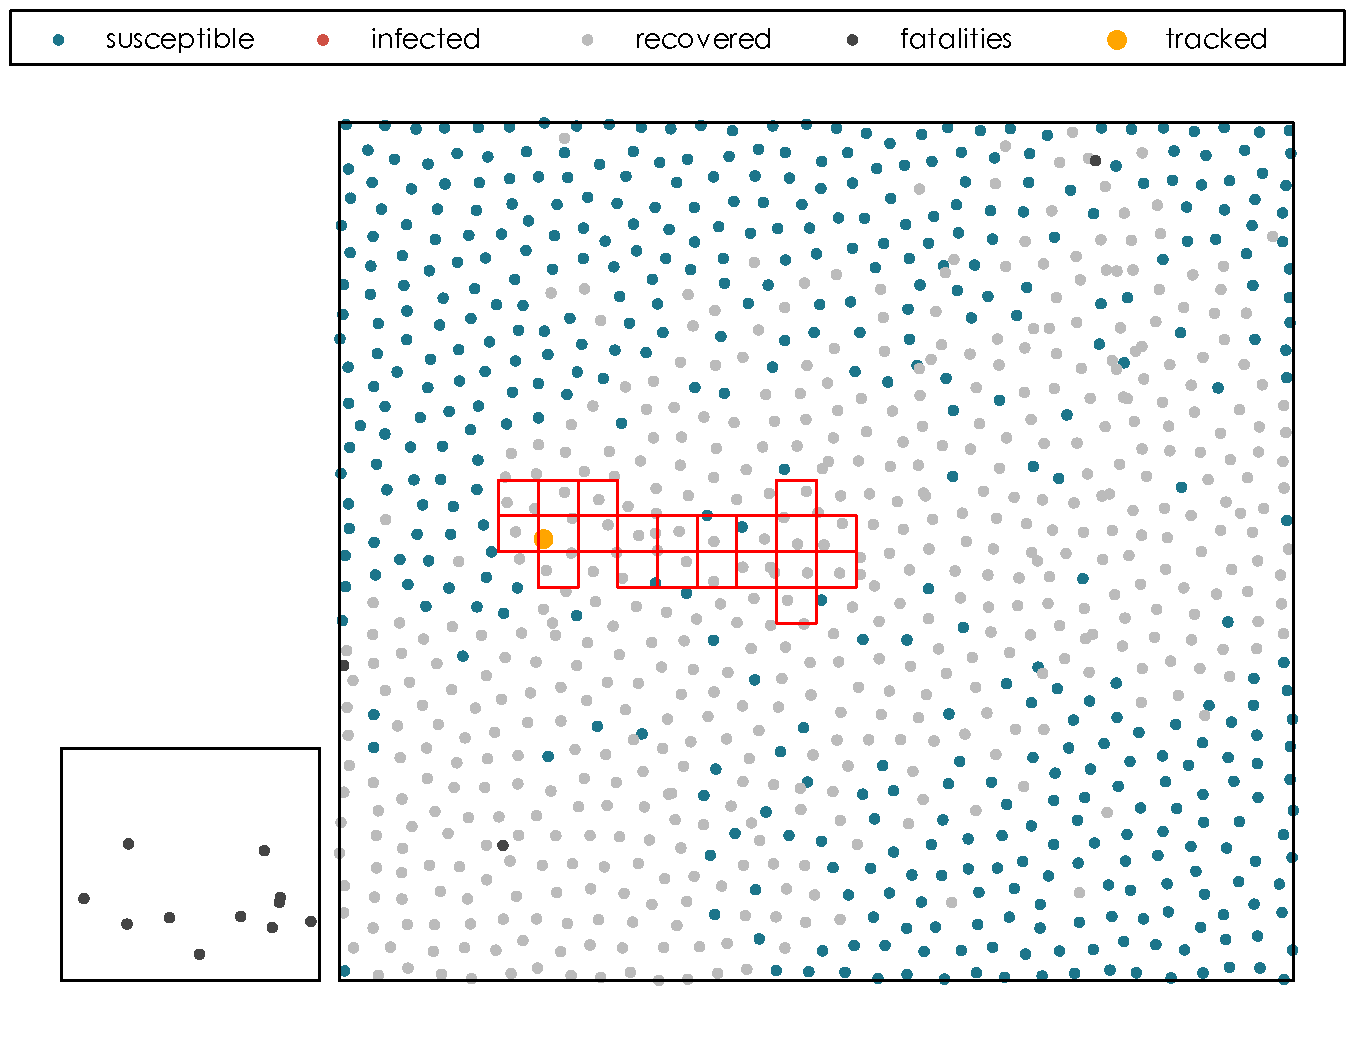
\includegraphics[width=0.95\textwidth]{render_1_restrictions/sim_3500.pdf}
						}%
					};
				\only<3-7>{\node[inner sep=0pt,align=flush center,above=\belowcaptionskip of abm,text width=\linewidth]
					{\vspace{-1em}{\large with intervention}};}%
				%
				\node [inner sep=0pt,above right, opacity=1.0]  at (0.0\textwidth,-0.69\textheight) (mobility) 
				{
					\only<8>{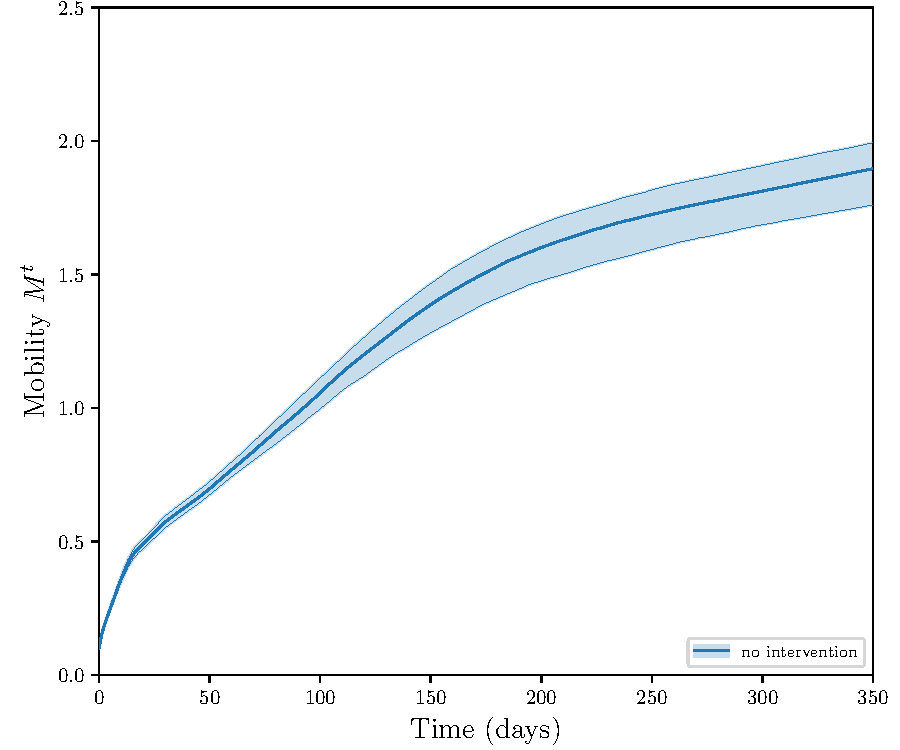
\includegraphics[width=0.9\textwidth]{trajectory_demo/M_compare_opt_1.pdf}}%
					\only<9>{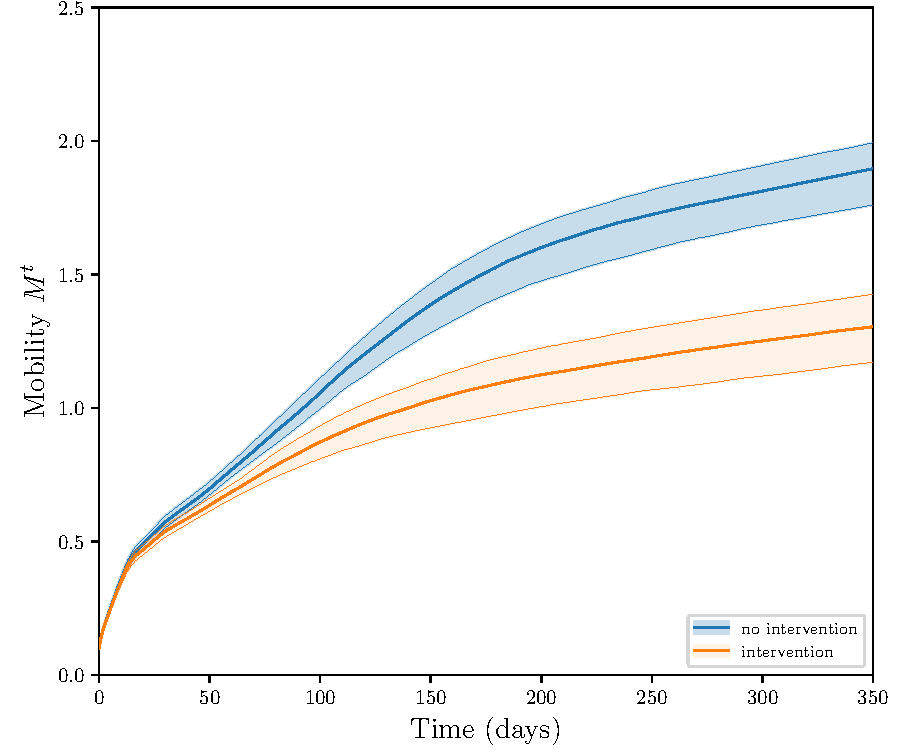
\includegraphics[width=0.9\textwidth]{trajectory_demo/M_compare_opt_3.pdf}}%
				};
				\only<3>{
					\node [draw=black, line width=0.1mm, fill=white, inner sep=5pt,above right, opacity=1.0]  at (0.5,-1.5) (text eworker) 
						{
							\Large essential workers
						};
					\node [above right] at (3,-3.5) (eworker) {};
					\draw[-stealth,line width=2pt] (text eworker.south) to [in=90,out=270] (eworker);
				}%
				\only<4>{
					\node [draw=black, line width=0.1mm, fill=white, inner sep=5pt,above right, opacity=1.0]  at (0.5,-1.5) (text hospital) 
						{
							\Large testing and quarantine
						};
					\node [above right] at (1,-4.5) (hospital) {};
					\draw[-stealth,line width=2pt] (text hospital.south) to [in=90,out=270] (hospital);
				}%
				\only<5>{
					\node [draw=black, line width=0.1mm, fill=white, inner sep=5pt,above right, opacity=1.0]  at (0.5,-1.5) (text sd) 
						{
							\Large social distancing
						};
					\node [above right] at (2.6,-4.7) (sd) {};
					\node [above right] at (2.2,-5.5) (a1) {};
					\node [above right] at (2.7,-4.5) (a2) {};
					\draw[-stealth,line width=2pt] (text sd.south) to [in=90,out=270] (sd);
					\draw[stealth-stealth,line width=2pt,red] (a1) to (a2);
				}%
				\only<9->{
					\node[inner sep=0pt,align=flush center,above=\belowcaptionskip of mobility,text width=\linewidth]
					{\vspace{-1em}{
						\large {\color{red} mobility $\downarrow$}
					}};
				}%
				% show origin
				% \fill (0,0) circle (2pt);
			\end{tikzpicture}%
		\end{column}

	\end{columns}
	\vspace{-3em}
\end{frame}
%------------------------------------------------
\begin{frame}[t,label=abm_4]
	\frametitle{Optimization problem}
	\tikzstyle{background grid}=[draw, black!50,step=.5cm]
	%
	\uncover<2->{No gradient information available, blackbox is expensive and \only<3->{\emphasis}{noisy}}\\
	%
	\begin{columns}[t] % The "c" option specifies centered vertical alignment while the "t" option is used for top vertical alignment
		\begin{column}{.42\textwidth} % Left column and width
			\vspace{-1.2em}
			% Optimization problem
			\begin{exampleblock}{Objective and constraints}
				\only<1-3>{
					\begin{equation*}
						\begin{aligned}
							& \underset{\mathbf{x}}{\text{min}}
							& & f(\mathbf{x}) = -M^{T}\\
							& \text{subject to}
							& & \uncover<2->{{c}(\mathbf{x}) \equiv n_{I,\text{max}} - H_{\text{max}} \le 0}\\
							& \text{where}
							& & \mathbf{x}=\left[n_E,S_D,n_T\right]^\mathit{T}\\
						\end{aligned}
					\end{equation*}
				}%
				\only<4->{
					\vspace{-1.2em}
					\begin{equation*}
						\begin{aligned}
							& \underset{\mathbf{x}}{\text{min}}
							& & f(\mathbf{x}) = \mathbb{E}_{\Theta}\left[{f}_{\Theta}(\mathbf{x}) = -M^{T}\right]\\
							& \text{subject to}
							& & {c}(\mathbf{x}) = \mathbb{E}_{\Theta}\left[{c}_{\Theta}(\mathbf{x}) \equiv n_{I,\text{max}} - H_{\text{max}}\right] \le 0\\
							& \text{where}
							& & \mathbf{x}=\left[n_E,S_D,n_T\right]^\mathit{T},{\color{red}\Theta\mathrm{:realizations}}
						\end{aligned}
					\end{equation*}
				}%
			\end{exampleblock}
			\vspace{-0.5em}
			\uncover<1->{
				% Variables
				\begin{alertblock}{Design variables}
					\vspace{-0.0em}
						\begin{itemize}\itemsep0em
							\item $n_E:$ Number of essential workers
							\item $S_D:$ Social distancing factor
							\item $n_T:$ Number of tests daily
						\end{itemize}
				\end{alertblock}
			}%
			\vspace{-0.5em}
			\uncover<5->{
				% Parameters
				\begin{blueblock}{Randomly seeded parameters}
					\vspace{-0.0em}
					\begin{itemize}\itemsep0em
						\item Initial conditions
						\item Interactions, demographics
					\end{itemize}
				\end{blueblock}
			}%
		\end{column}
		%
		\begin{column}{.5\textwidth} % Left column and width
			\tikzstyle{background grid}=[draw, black!50,step=.5cm]
			\begin{tikzpicture}[remember picture, overlay]%[show background grid]
				\only<1-5>{
					\node [inner sep=0pt,above right, opacity=1.0] at (0, -4.5) (objective)
						{
							\only<1->{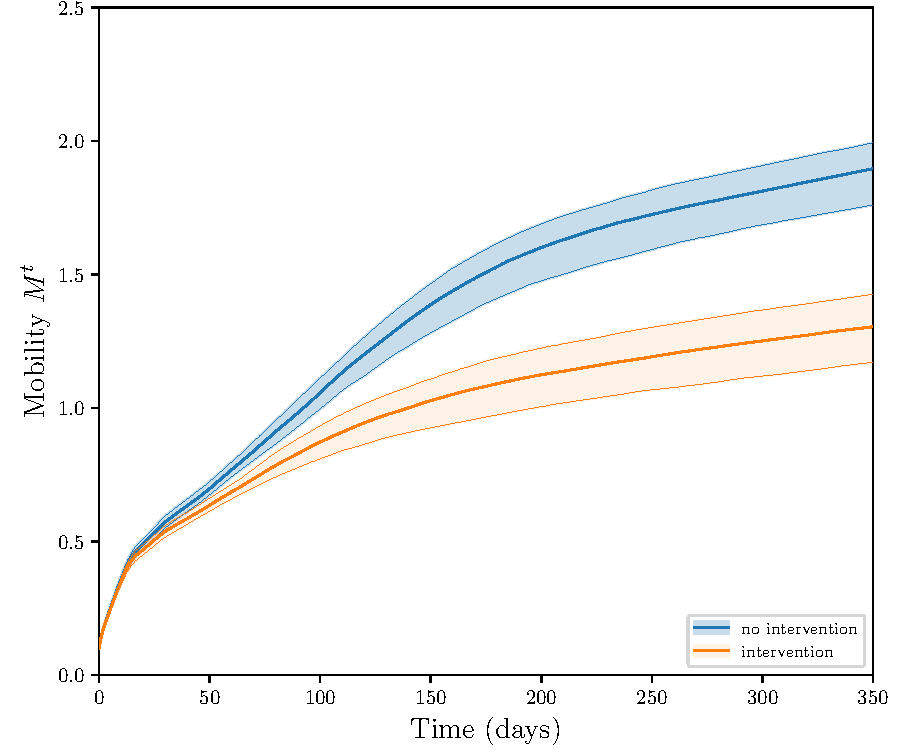
\includegraphics[width=0.7\textwidth]{trajectory_demo/M_compare_opt_3.pdf}}%
						};
					\only<1->{
						\node [above right] at (3.2,-3.5) (a1) {};
						\node [above right] at (2.2,-1.5) (a2) {};
						\draw[-stealth,line width=2pt,black] (a1) to [out=90, in=310] (a2);
					}
					\node [inner sep=0pt,above right, opacity=0.7] at (2.5, -6.5) (constraint)
						{
							\only<2->{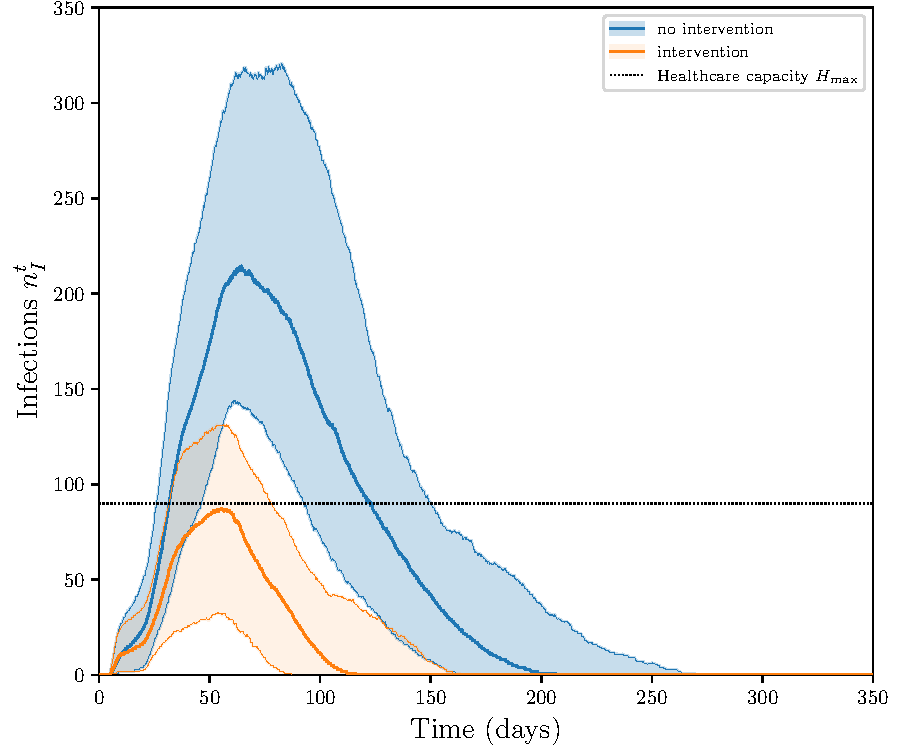
\includegraphics[width=0.7\textwidth]{trajectory_demo/I_compare_opt_3.pdf}}%
						};
					\only<2->{
						\node [above right] at (4.7,-3.5) (a1) {};
						\node [above right] at (3.7,-5.5) (a2) {};
						\draw[-stealth,line width=2pt,black] (a1) to [out=210, in=90] (a2);
					}					

				}%
				% show origin
				% \fill (0,0) circle (2pt);
				% define destination coordinates
			\end{tikzpicture}%
		\end{column}
	
	\end{columns}
	\vspace{-3em}
\end{frame}

% Section 04: results
%------------------------------------------------
\section{Optimization results}
%------------------------------------------------
\begin{frame}[t]
	\frametitle{Optimization results}
	\tikzstyle{background grid}=[draw, black!50,step=.5cm]
	%
	\uncover<1->{StoMADS, \texttt{NOMAD}\ifshowcitations\footpartcite{NOMAD}\fi, and genetic algorithms were used to solve the problem\ifshowcitations\footpartcite{Alhandawi2021b}\fi}\\
	%
	\begin{columns}[t] % The "c" option specifies centered vertical alignment while the "t" option is used for top vertical alignment
		\begin{column}{.42\textwidth} % Left column and width
			\vspace{-1.2em}
			% Optimization problem
			\begin{exampleblock}{Objective and constraints}
				\vspace{-1.2em}
				\begin{equation*}
					\begin{aligned}
						& \underset{\mathbf{x}}{\text{min}}
						& & f(\mathbf{x}) = \mathbb{E}_{\Theta}\left[{f}_{\Theta}(\mathbf{x}) = -M^{T}\right]\\
						& \text{subject to}
						& & {c}(\mathbf{x}) = \mathbb{E}_{\Theta}\left[{c}_{\Theta}(\mathbf{x}) \equiv n_{I,\text{max}} - H_{\text{max}}\right] \le 0\\
						& \text{where}
						& & \mathbf{x}=\left[n_E,S_D,n_T\right]^\mathit{T},\Theta\mathrm{:realizations}
					\end{aligned}
				\end{equation*}
			\end{exampleblock}
			\vspace{-0.5em}
			% Variables
			\begin{alertblock}{Design variables}
				\vspace{-0.0em}
					\begin{itemize}\itemsep0em
						\item $n_E:$ Number of essential workers
						\item $S_D:$ Social distancing factor
						\item $n_T:$ Number of tests daily
					\end{itemize}
			\end{alertblock}
			\vspace{-0.5em}
			% Parameters
			\begin{blueblock}{Randomly seeded parameters}
				\vspace{-0.0em}
				\begin{itemize}\itemsep0em
					\item Initial conditions
					\item Interactions, demographics
				\end{itemize}
			\end{blueblock}
		\end{column}
		%
		\begin{column}{.5\textwidth} % Left column and width
			\tikzstyle{background grid}=[draw, black!50,step=.5cm]
			\begin{tikzpicture}[remember picture, overlay]%[show background grid]
				\node [inner sep=0pt, opacity=1.0,minimum size=10cm]  at (0.47\textwidth,-0.05\textheight) (mobility) 
				{	
					\centering
					\only<2>{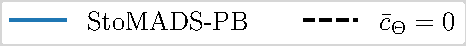
\includegraphics[height=12pt]{results_opt_traces/legend_0.pdf}}%
					\only<3>{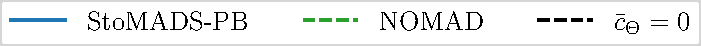
\includegraphics[height=12pt]{results_opt_traces/legend_1.pdf}}%
					\only<4->{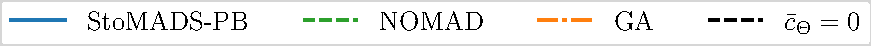
\includegraphics[height=12pt]{results_opt_traces/legend_2.pdf}}%
				};
				\node [inner sep=0pt,above right, opacity=1.0]  at (0.0\textwidth,-0.69\textheight) (mobility) 
				{
					\only<2>{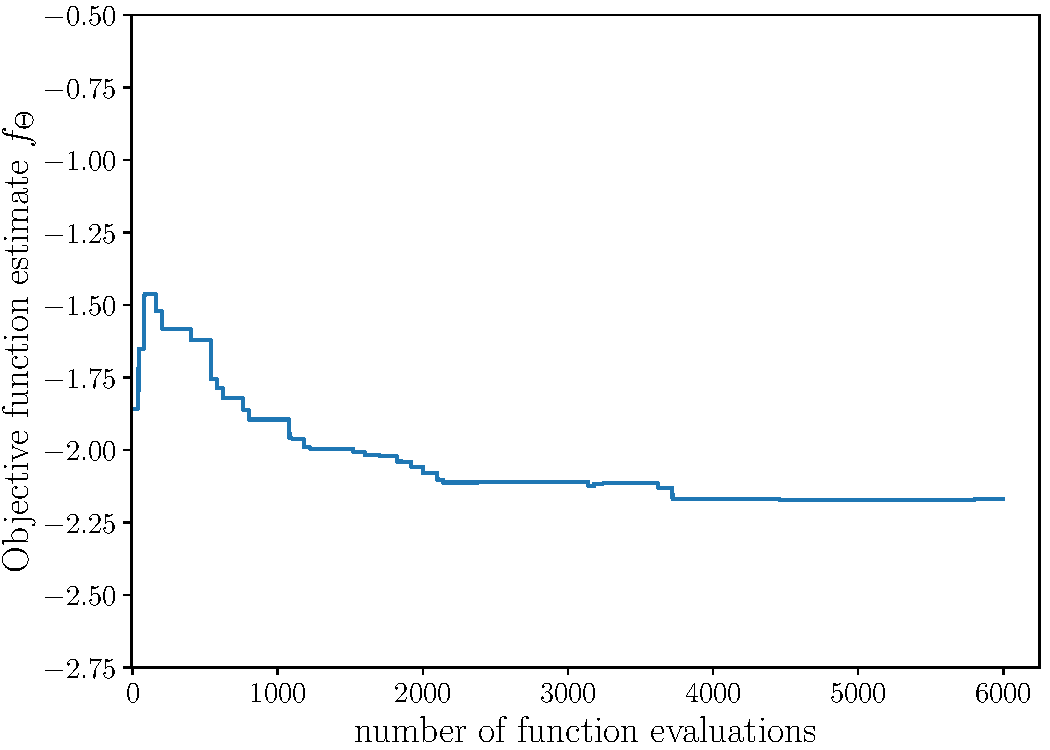
\includegraphics[width=0.95\textwidth]{results_opt_traces/f_nk=20_0.pdf}}%
					\only<3>{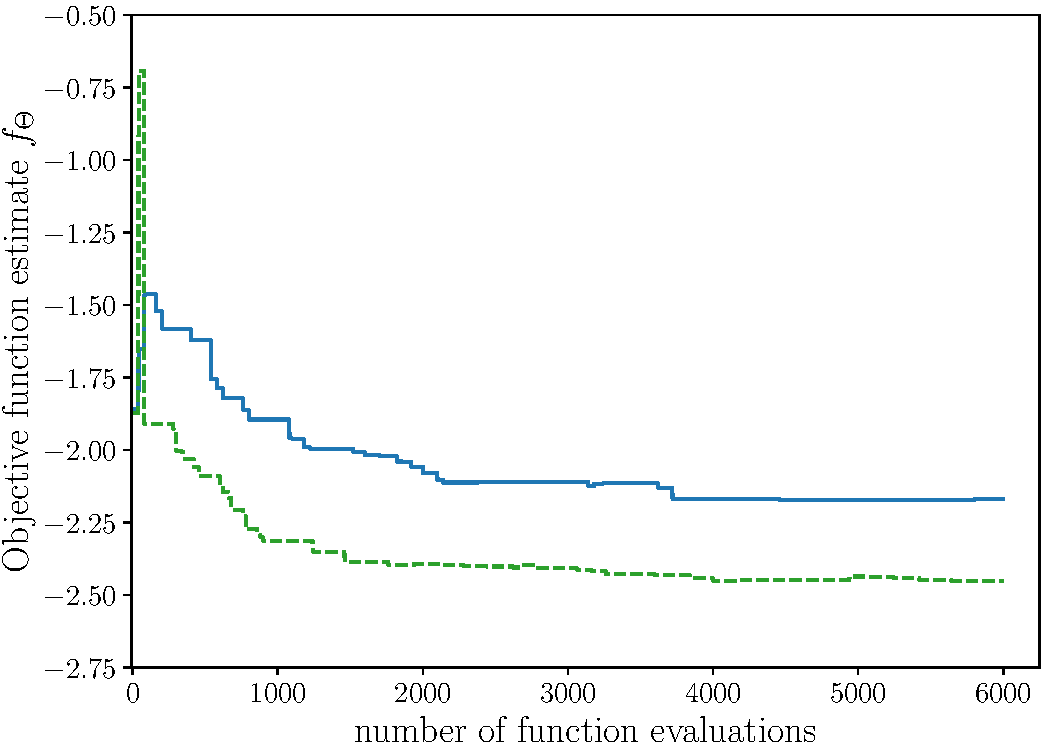
\includegraphics[width=0.95\textwidth]{results_opt_traces/f_nk=20_1.pdf}}%
					\only<4>{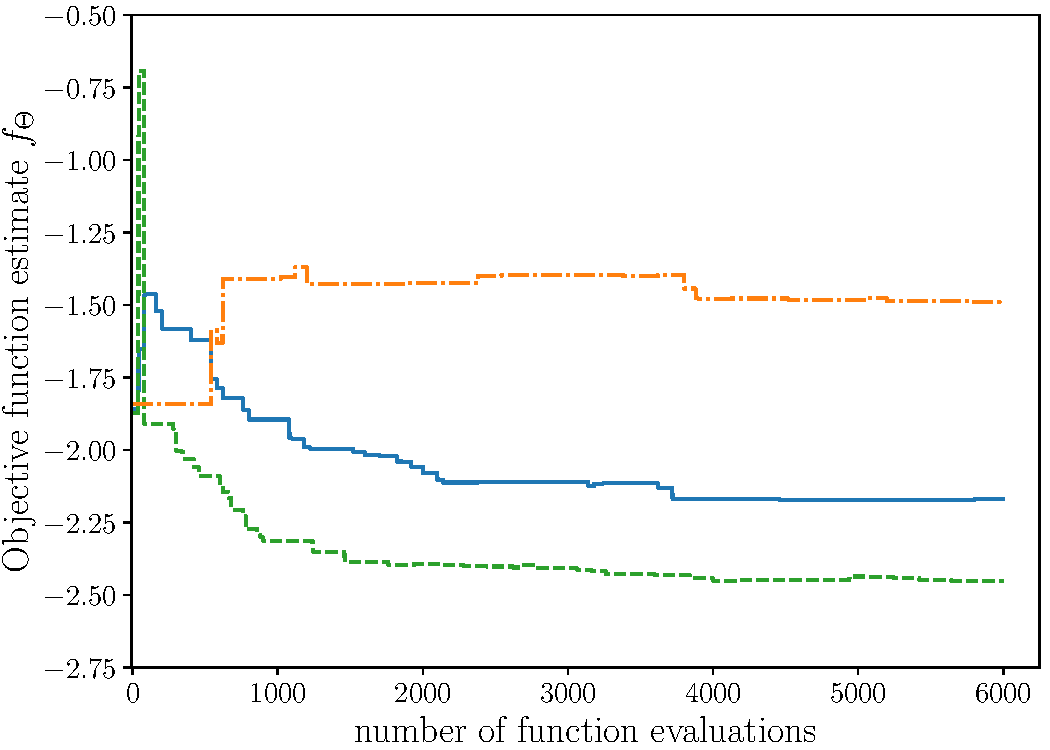
\includegraphics[width=0.95\textwidth]{results_opt_traces/f_nk=20_2.pdf}}%
					\only<5>{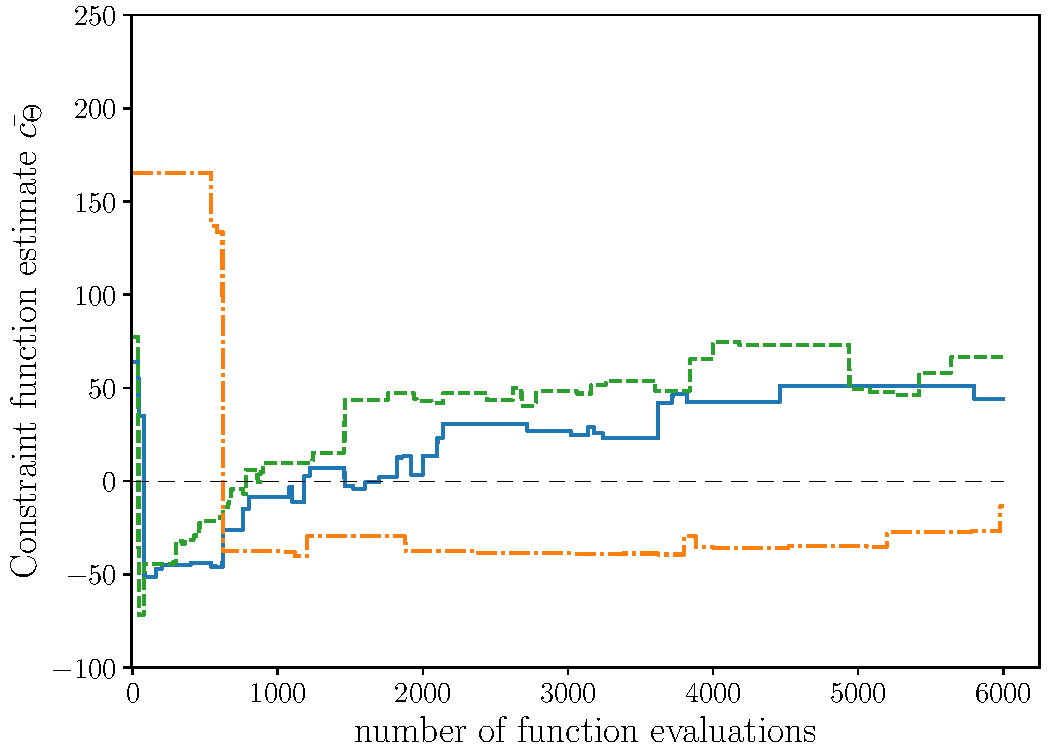
\includegraphics[width=0.95\textwidth]{results_opt_traces/g_nk=20_2.pdf}}%
				};
				\only<2-5>{
					\node[inner sep=0pt,align=flush center,above=\belowcaptionskip of mobility,text width=\linewidth]
					{\vspace{1em}{
						\large sampling rate $n^k=4$
					}};
				}%
				% show origin
				% \fill (0,0) circle (2pt);
			\end{tikzpicture}%
			\begin{tikzpicture}[remember picture, overlay]%[show background grid]
				\node [inner sep=0pt,above right, opacity=1.0]  at (0.0\textwidth,-0.75\textheight) (mobility) 
				{
					\only<6>{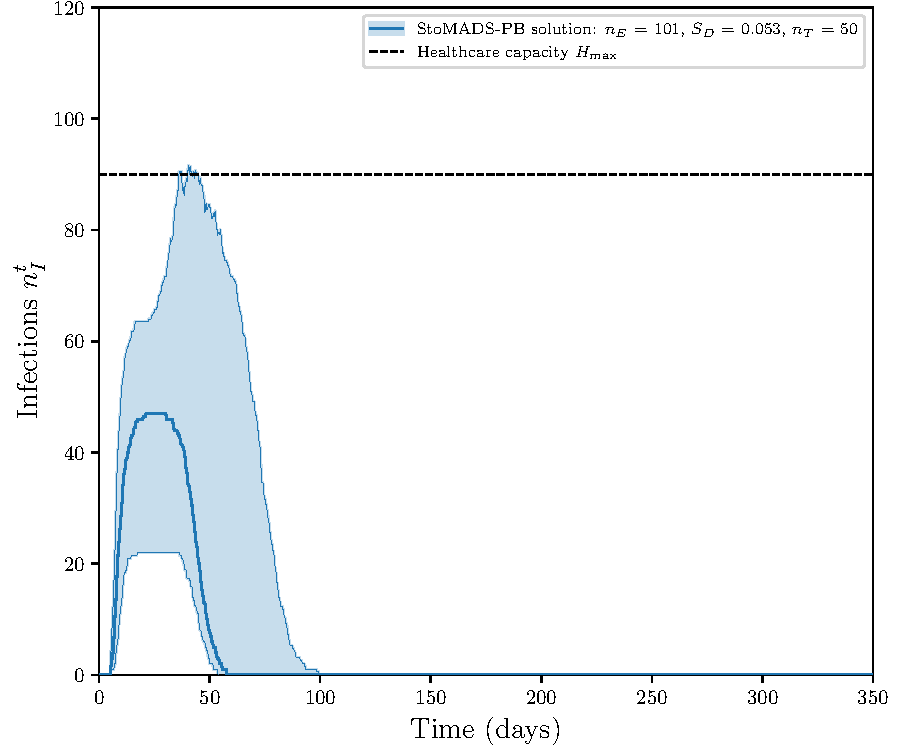
\includegraphics[width=0.93\textwidth]{trajecctory_results/I_compare_opt_0.pdf}}%
					\only<7>{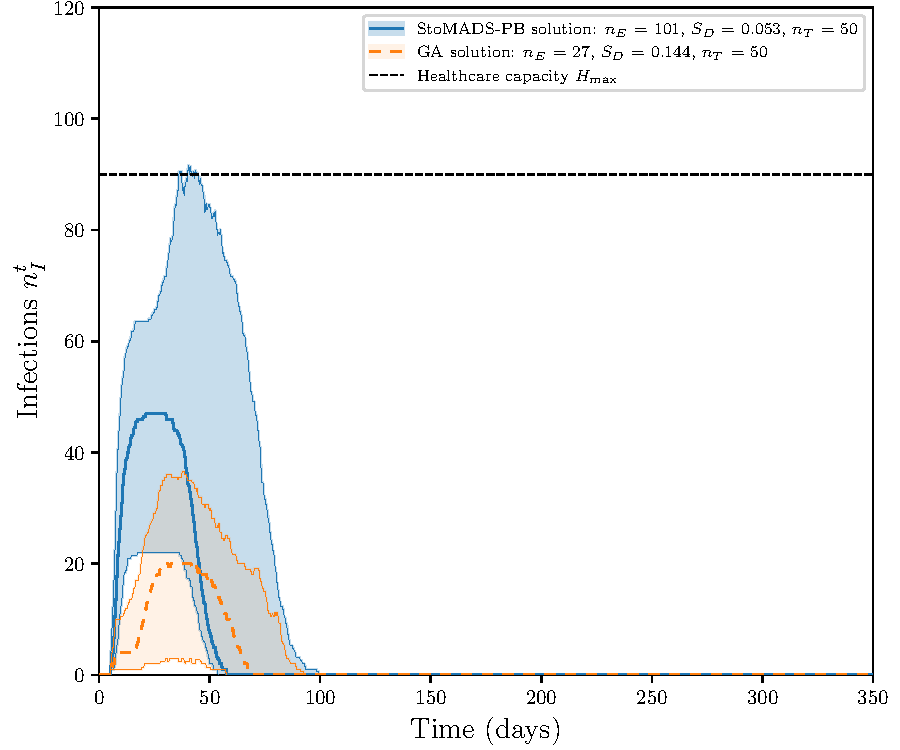
\includegraphics[width=0.93\textwidth]{trajecctory_results/I_compare_opt_1.pdf}}%
					\only<8>{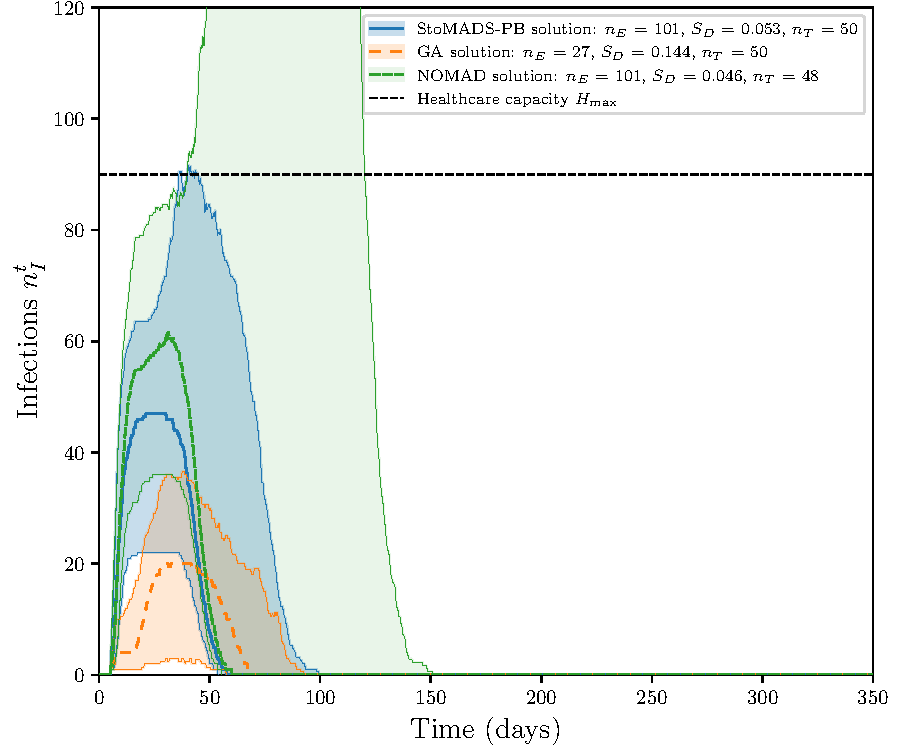
\includegraphics[width=0.93\textwidth]{trajecctory_results/I_compare_opt_2.pdf}}%
					\only<9>{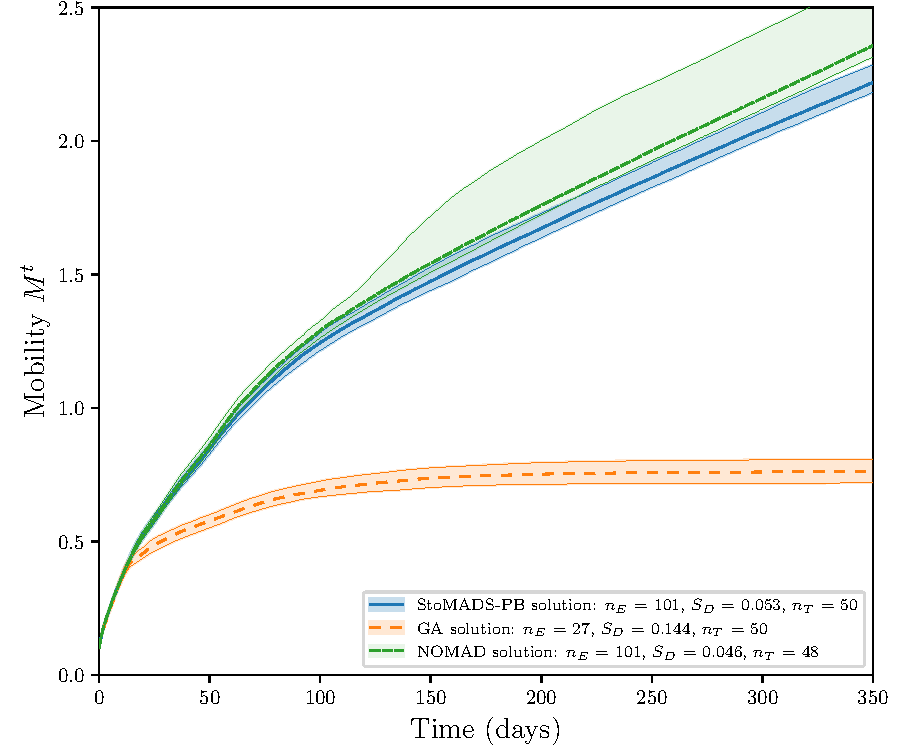
\includegraphics[width=0.93\textwidth]{trajecctory_results/M_compare_opt_2.pdf}}%
				};
				\only<6->{
					\node[inner sep=0pt,align=flush center,above=\belowcaptionskip of mobility,text width=\linewidth]
					{\vspace{1em}{
						\large best known solution
					}};
				}%
				% show origin
				% \fill (0,0) circle (2pt);
			\end{tikzpicture}%
		\end{column}
	
	\end{columns}
	\vspace{-3em}
\end{frame}
\addtocounter{footnote}{-2}
%------------------------------------------------

% Section 05: conclusion
%------------------------------------------------

\section{Conclusion}
%------------------------------------------------
\begin{frame}[t,label=abm_7]
	\frametitle{Conclusion}
	\tikzstyle{background grid}=[draw, black!50,step=.5cm]
	%
	\uncover<1->{Formulated and solved public health policy-making problems}%
	\only<6->{{\color{white}\ifshowcitations\footpartcite{Ferguson2020}\fi}}\\
	%
	\begin{columns}[t] % The "c" option specifies centered vertical alignment while the "t" option is used for top vertical alignment
		\begin{column}{.42\textwidth} % Left column and width
			\begin{itemize}
				\item<1-> Identified a public health policy that favored
				\begin{itemize}
					\item<2-> High testing capacity $n_T$
					\item<3-> Large number of essential workers $n_E$
					\item<4-> Modest social distancing $S_D$
				\end{itemize}
				\item<5-> StoMADS outperformed GAs and NOMAD on active constraints
				\item<6-> Applicable to other large-scale agent-based models\footnotemark[1]
			\end{itemize}
		\end{column}
		%
		\begin{column}{.5\textwidth} % Left column and width
			\tikzstyle{background grid}=[draw, black!50,step=.5cm]
			\begin{tikzpicture}[remember picture, overlay]%[show background grid]
				\node [inner sep=0pt,above right, opacity=1.0]  at (0.0\textwidth,-0.75\textheight) (mobility) 
				{
					\only<-5>{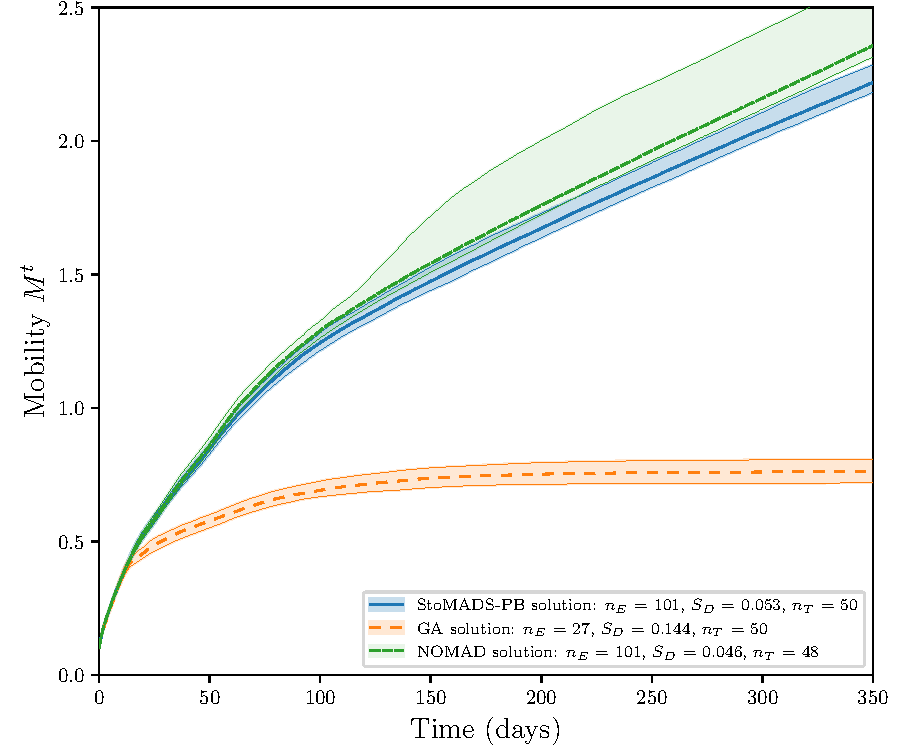
\includegraphics[width=0.93\textwidth]{trajecctory_results/M_compare_opt_2.pdf}}%
				};
				\only<-5>{
					\node[inner sep=0pt,align=flush center,above=\belowcaptionskip of mobility,text width=\linewidth]
					{\vspace{-0em}{
						\large best known solution
					}};
				}%
				% show origin
				% \fill (0,0) circle (2pt);
			\end{tikzpicture}%
			\begin{tikzpicture}[remember picture, overlay] %show background grid, 
				\node [inner sep=0pt,above right, opacity=1.0]  at (0.1\textwidth,-0.66\textheight) (abm) 
					{
						\only<6>{
							\begin{animateinline}[autoplay,width=0.9\textwidth]{8}
								\ifshowanimations
									\multiframe{48}{i=1+15}{%
										\includegraphics{canada_ABM/map_\i.png}
									}
								\else
									\multiframe{1}{i=721+0}{%
										\includegraphics{canada_ABM/map_\i.png}
									}
								\fi
							\end{animateinline}%
						}%
						\only<7->{
							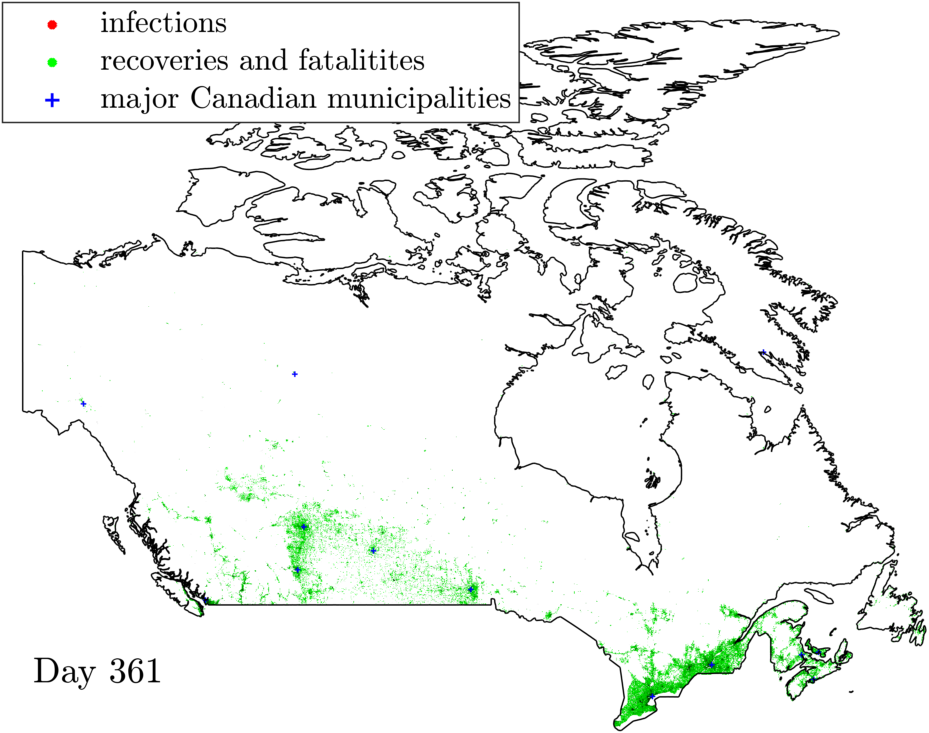
\includegraphics[width=0.9\textwidth]{canada_ABM/map_721.png}
						}
					};
			\end{tikzpicture}%
		\end{column}
	
	\end{columns}
	\vspace{-3em}
\end{frame}
\addtocounter{footnote}{-1}

%----------------------------------------------------------------------------------------
%	PRESENTATION SLIDES
%----------------------------------------------------------------------------------------

% Section 01: background
%------------------------------------------------
\section{Introduction}
%------------------------------------------------
\begin{frame}[t]
	\frametitle{Background: COVID-19 forecasting targets}
	\tikzstyle{background grid}=[draw, black!50,step=.5cm]
	%
	Forecasting novel epidemics is a multidisciplinary field involving multiple \emph{targets} \footpartcite{Wu2021}\\
	\emph{Inputs} for forecasting \emphasis{epidemic size:}\\
    %
    \begin{itemize}
        \item<2-> Growth rate indicators
        \item<3-> \only<5->{\emphasis}{Historical incidence rate data}
        \item<4-> \only<5->{\emphasis}{Serologic assays}\\
        \centering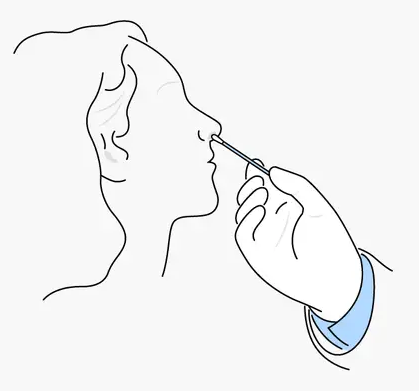
\includegraphics[width=0.23\textwidth]{targets/pcr.png}
    \end{itemize}
    %
	\tikzstyle{background grid}=[draw, black!50,step=.5cm]
	\begin{tikzpicture}[remember picture, overlay] %show background grid, 
		% Put the graphic inside a node. This makes it easy to place the
		% graphic and to draw on top of it. 
		% The above right option is used to place the lower left corner
		% of the image at the (0,0) coordinate. 
		\node [inner sep=0pt,above left, opacity=1.0]  at (0.99\textwidth,-0.0\textheight) (seq2seq) 
			{
				\only<1>{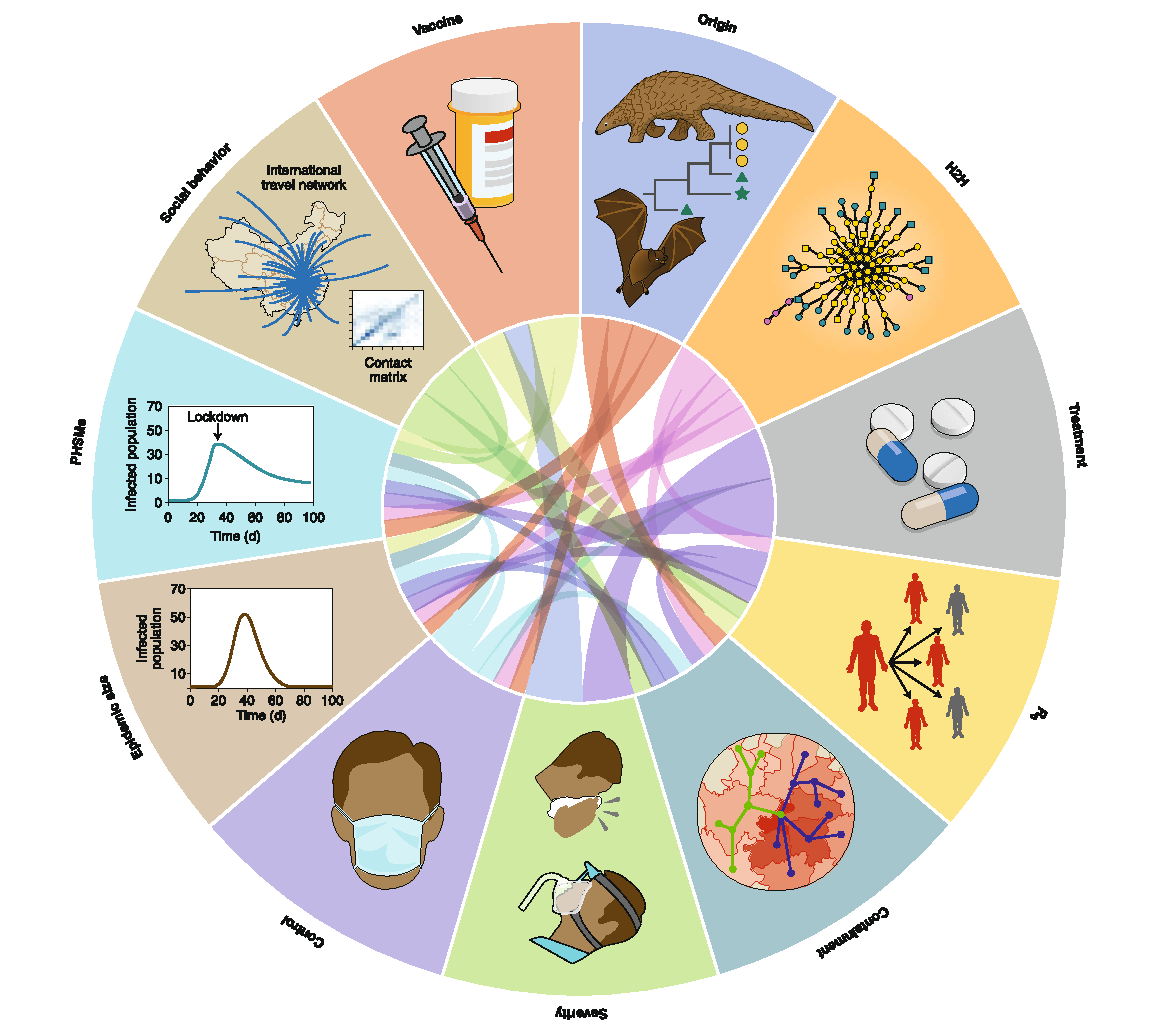
\includegraphics[width=0.45\textwidth]{targets/nowcasting_targets_1.pdf}}%
				\only<2>{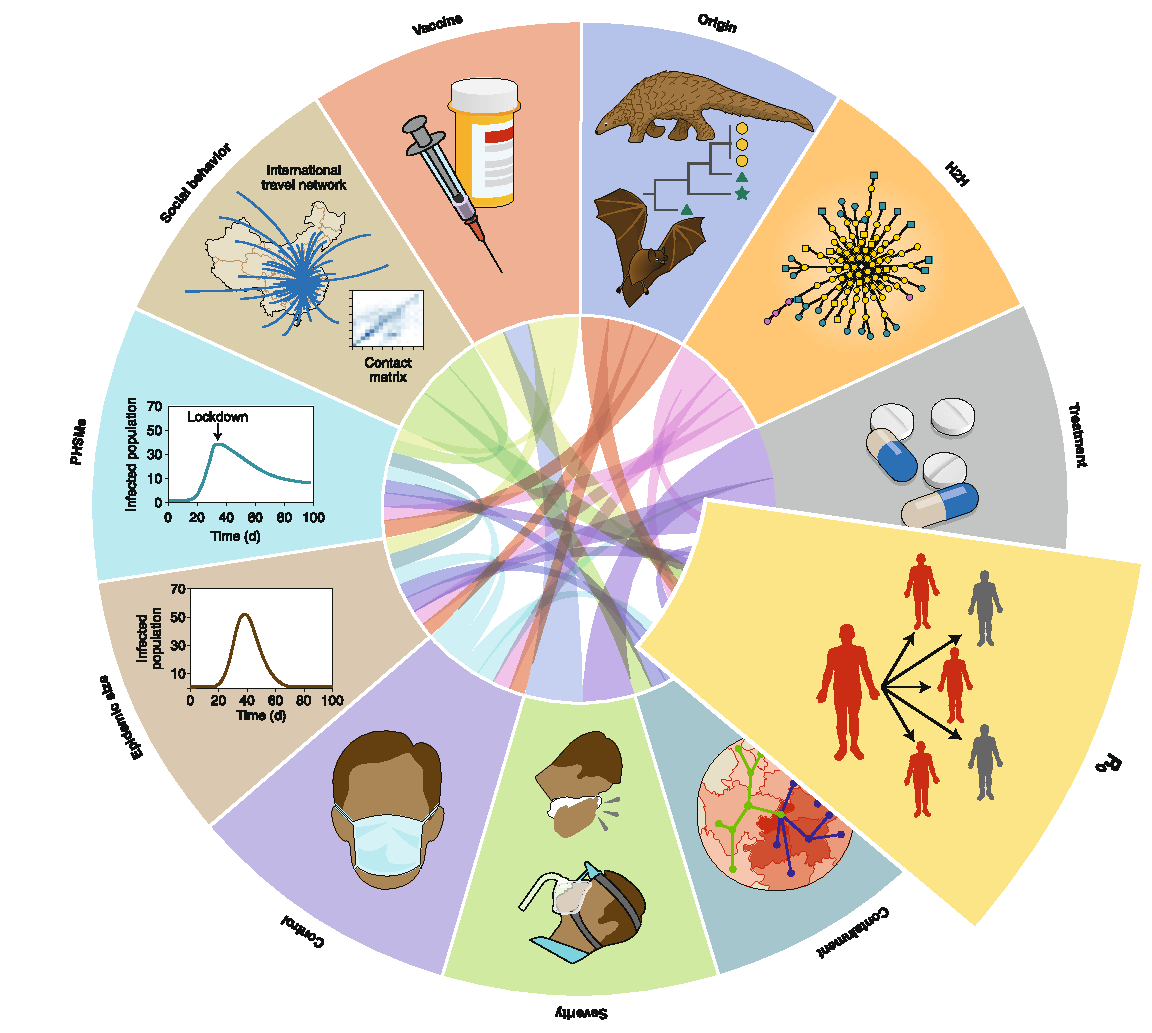
\includegraphics[width=0.45\textwidth]{targets/nowcasting_targets_2.pdf}}%
                \only<3->{\includegraphics[width=0.45\textwidth]{targets/nowcasting_targets_3.pdf}}%
			};
		\only<1->{
			\node[inner sep=0pt,below=\belowcaptionskip of seq2seq,text width=\linewidth]
				{\vspace{-1em}{Nowcasting targets}};
		}%
		% show origin
		% \fill (0,0) circle (2pt);
	\end{tikzpicture}%
	%
	\vspace{-3em}
\end{frame}
\addtocounter{footnote}{-1}
%------------------------------------------------

% Section 02: motivation
%------------------------------------------------
\section{Overview of problem}
%------------------------------------------------
\begin{frame}[t]
	\frametitle{COVID-19 incidence forecasting}
	\tikzstyle{background grid}=[draw, black!50,step=.5cm]
	%
	How to \emph{design} a machine learning model for forecasting a time-series?\\
	%
	\tikzstyle{background grid}=[draw, black!50,step=.5cm]
	\begin{tikzpicture}[remember picture, overlay] %show background grid, 
		% Put the graphic inside a node. This makes it easy to place the
		% graphic and to draw on top of it. 
		% The above right option is used to place the lower left corner
		% of the image at the (0,0) coordinate. 
		\node [inner sep=0pt,above right, opacity=1.0]  at (0.0\textwidth,-0.72\textheight) (raw data) 
			{
				\only<1>{\includegraphics[width=0.43\textwidth]{raw_data/animation_0.pdf}}%
				\only<2>{\includegraphics[width=0.43\textwidth]{raw_data/animation_1.pdf}}%
				\only<3>{\includegraphics[width=0.43\textwidth]{raw_data/animation_2.pdf}}%
				\only<4->{\includegraphics[width=0.43\textwidth]{raw_data/animation_3.pdf}}%
			};
		\node [inner sep=0pt,above left, opacity=1.0]  at (0.99\textwidth,-0.65\textheight) (seq2seq) 
			{
				\only<5>{\includegraphics[width=0.55\textwidth]{model_1.pdf}}%
				\only<6>{\includegraphics[width=0.55\textwidth]{model_2.pdf}}%
				\only<7>{\includegraphics[width=0.55\textwidth]{model_3.pdf}}%
			};
		% \only<5->{
		% 	\node[inner sep=0pt,below=\belowcaptionskip of seq2seq,text width=\linewidth]
		% 		{\vspace{-1em}{Seq2Seq model}};
		% }%
		\node [inner sep=0pt, opacity=1.0]  at (0.43\textwidth,-0.15\textheight) (ct) {};%
		\node [inner sep=0pt, opacity=1.0]  at (0.43\textwidth,-0.50\textheight) (cases) {};%
		\only<-6>{
			\node [inner sep=0pt, opacity=1.0]  at (0.65\textwidth,-0.50\textheight) (input) {};%
		}%
		\only<7->{
			\node [inner sep=0pt, opacity=1.0]  at (0.60\textwidth,-0.60\textheight) (input) {};%
		}%
		% show origin
		% \fill (0,0) circle (2pt);
	\end{tikzpicture}%
	%
	\begin{tikzpicture}[overlay]
		\only<5->{\path[->,magenta,thick] (ct) edge [out=0, in=270] (input);}
		\only<5->{\path[->,magenta,thick] (cases) edge [out=0, in=270] (input);}
	\end{tikzpicture}%
	%
	\vspace{-3em}
\end{frame}


% Section 03: hyperparameters
%------------------------------------------------
\section{Hyperparameter tuning}
%------------------------------------------------
\begin{frame}[t]
    \frametitle{Training the model}
	%
	There are several challenges associated with hyperparameter optimization\\
	%
    \begin{columns}[t] % The "c" option specifies centered vertical alignment while the "t" option is used for top vertical alignment
		
        \begin{column}{.5\textwidth} % Left column and width
        \only<1->{
			\begin{itemize}
				\item The number of epochs can be tuned using \textit{early stopping}%
				\item This is a form of \textit{regularization} to reduce over-fitting%
			\end{itemize}
        }%
        \only<3->{
			~~~However,\\
			\uncover<4->{
				~~~1) Other hyperparameters to tune
				\begin{itemize}
					\item Dropout%
					\item Training batch size%
					\item Activation function(s)%
				\end{itemize}
			}%
            \uncover<5->{~~~2) Training can be \emphasis{expensive}}\\
            \uncover<6->{~~~3) Backpropagation is \emphasis{stochastic}}
        }%
    
        \end{column}
    
        \begin{column}{.5\textwidth} % Left column and width
    
            \vspace{-1.5em}
            \begin{figure}
                \centering
                \only<1>{\includegraphics[width=0.9\textwidth]{training/epoch_0.pdf}}%
                \only<2>{
					\begin{animateinline}[autoplay,width=0.9\textwidth]{8}
						\ifshowanimations
							\multiframe{52}{i=0+5}{%
								\includegraphics{training/epoch_\i.pdf}
							}
						\else
							\multiframe{1}{i=262+0}{%
								\includegraphics{training/epoch_\i.pdf}
							}
						\fi
					\end{animateinline}%
                }%
                \only<3->{\includegraphics[width=0.9\textwidth]{training/final_model.pdf}}%
                \vspace{-0.75em}
                \caption{Effect of number of epochs on testing loss}
            \end{figure}%
        \end{column}
    \end{columns}
        
\end{frame}
%------------------------------------------------
\begin{frame}[t]
	\frametitle{Hyperparameter tuning}
	\tikzstyle{background grid}=[draw, black!50,step=.5cm]
	%
	We can use StoMADS to solve such hyperparameter optimization problems \ifshowcitations\footpartcite{Khalil2021}\fi\\
	%
	\tikzstyle{background grid}=[draw, black!50,step=.5cm]
	\begin{tikzpicture}[remember picture, overlay] %show background grid, 
		% Put the graphic inside a node. This makes it easy to place the
		% graphic and to draw on top of it. 
		% The above right option is used to place the lower left corner
		% of the image at the (0,0) coordinate. 
		\node [inner sep=0pt,above right, opacity=1.0]  at (-0.01\textwidth,-0.7\textheight) (error) 
			{
				\only<1>{\includegraphics[width=0.5\textwidth]{box_plots/boxplot_input_dim_0.pdf}}%
				\only<2>{\includegraphics[width=0.5\textwidth]{box_plots/boxplot_input_dim_1.pdf}}%
				\only<3>{\includegraphics[width=0.5\textwidth]{box_plots/boxplot_input_dim_2.pdf}}%
				\only<4>{\includegraphics[width=0.5\textwidth]{box_plots/boxplot_input_dim_3.pdf}}%
				\only<5>{\includegraphics[width=0.5\textwidth]{box_plots/boxplot_input_dim_4.pdf}}%
				\only<6>{\includegraphics[width=0.5\textwidth]{box_plots/boxplot_input_dim_5.pdf}}%
				\only<7>{\includegraphics[width=0.5\textwidth]{box_plots/boxplot_input_dim_6.pdf}}%
				\only<8>{\includegraphics[width=0.5\textwidth]{box_plots/boxplot_input_dim_opt.pdf}}%
				\only<9>{\includegraphics[width=0.5\textwidth]{box_plots/boxplot_hid_dim_opt.pdf}}%
				\only<10>{\includegraphics[width=0.5\textwidth]{box_plots/boxplot_dropout_opt.pdf}}%
			};
		\node [inner sep=0pt,above left, opacity=1.0]  at (1.01\textwidth,-0.7\textheight) (prediction) 
			{
				\only<1>{\includegraphics[width=0.5\textwidth]{models/model_input_dim_0.pdf}}%
				\only<2>{\includegraphics[width=0.5\textwidth]{models/model_input_dim_1.pdf}}%
				\only<3>{\includegraphics[width=0.5\textwidth]{models/model_input_dim_2.pdf}}%
				\only<4>{\includegraphics[width=0.5\textwidth]{models/model_input_dim_3.pdf}}%
				\only<5>{\includegraphics[width=0.5\textwidth]{models/model_input_dim_4.pdf}}%
				\only<6>{\includegraphics[width=0.5\textwidth]{models/model_input_dim_5.pdf}}%
				\only<7>{\includegraphics[width=0.5\textwidth]{models/model_input_dim_6.pdf}}%
				\only<8>{\includegraphics[width=0.5\textwidth]{models/final_model_input_dim.pdf}}%
				\only<9>{\includegraphics[width=0.5\textwidth]{models/final_model_hid_dim.pdf}}%
				\only<10->{\includegraphics[width=0.5\textwidth]{models/final_model_dropout.pdf}}%
			};
		% show origin
		% \fill (0,0) circle (2pt);
	\end{tikzpicture}%
	%
	\begin{columns}[t] % The "c" option specifies centered vertical alignment while the "t" option is used for top vertical alignment
		\begin{column}{.42\textwidth} % Left column and width
			\vspace{-2.0em}
			% Optimization problem
			\uncover<11->{
				\begin{exampleblock}{Objective and constraints}
					\vspace{-0.0em}
					\begin{equation*}
						\begin{aligned}
							& \underset{\mathbf{x}}{\text{min}}
							& & f(\mathbf{x}) = \mathbb{E}_{\Theta}\left[{f}_{\Theta}(\mathbf{x}) = \mathrm{error}_\mathrm{CV}\right]\\
							& \text{where}
							& & \Theta\mathrm{:realizations}
						\end{aligned}
					\end{equation*}
				\end{exampleblock}
			}%
			\vspace{-0.5em}
			\uncover<11->{
				% Variables
				\begin{alertblock}{Design variables ($\mathbf{x}$)}
					\vspace{-0.0em}
						\begin{itemize}\itemsep0em
							\item $T_1:$ Input dimension
							\item $n_\text{hidden}:$ Number of hidden neurons
							\item $P_\text{dropout}:$ Probability of dropout, etc.
						\end{itemize}
				\end{alertblock}
			}%
			\vspace{-0.5em}
			\uncover<11->{
				% Parameters
				\begin{blueblock}{Randomly seeded parameters}
					\vspace{-0.0em}
					\begin{itemize}\itemsep0em
						\item Initial weights
						\item Gradient descent steps
					\end{itemize}
				\end{blueblock}
			}%
		\end{column}
		%
		\begin{column}{.5\textwidth} % Left column and width
		\end{column}
	
	\end{columns}
	%
	\vspace{-3em}
\end{frame}
\addtocounter{footnote}{-1}
%------------------------------------------------

% Section 04: results
%------------------------------------------------
\section{Results}
%------------------------------------------------
\subsection{Optimal hyperparameters}
\begin{frame}[t]
	\frametitle{Results: Optimal hyperparameters}
	\tikzstyle{background grid}=[draw, black!50,step=.5cm]
	%
	Optimal hyperparameters for the \emph{Seq2Seq} model:\\
	%
	\tikzstyle{background grid}=[draw, black!50,step=.5cm]
	\begin{tikzpicture}[remember picture, overlay] %show background grid, 
		% Put the graphic inside a node. This makes it easy to place the
		% graphic and to draw on top of it. 
		% The above right option is used to place the lower left corner
		% of the image at the (0,0) coordinate. 
		\node [inner sep=0pt,above left, opacity=1.0]  at (1.01\textwidth,-0.73\textheight) (prediction) 
			{\includegraphics[width=0.5\textwidth]{predictions/model_predictions_test_S2S_mean_Ct_daily_cases.pdf}};
		% show origin
		% \fill (0,0) circle (2pt);
	\end{tikzpicture}%
	%
	\begin{columns}[t] % The "c" option specifies centered vertical alignment while the "t" option is used for top vertical alignment
		\begin{column}{.42\textwidth} % Left column and width
			\vspace{-2.0em}
            % Column widths
            \newcommand{\ocwb}{3.7cm}
            \newcommand{\ocwc}{1cm}
            \newcommand{\ocwd}{1.2cm}
            \newcommand{\ocwe}{3cm}
            %
            \begin{table}[h!]
                \centering
                \footnotesize
                \renewcommand{\arraystretch}{1.5}% Wider
                \begin{tabular}{L{\ocwb}C{\ocwc}C{\ocwd}} \toprule
                    \multicolumn{2}{c}{\bf Hyperparameter}	& \bf Value         \\ \toprule
                    Sliding window size  		& \Ti		&	6				\\
                    Number of hidden neurons	& \nh		&	1500			\\
                    Probability of dropout		& \Pd		&	0.8				\\
                    Number of hidden layers		& \nh		&	2				\\
                    Teacher forcing probability	& \Pt		&	0.3				\\
                    Learning rate 				& \lr		&	$1\times10^{-4}$\\
                    batch size 					& \bs		&	32				\\\hline
                \end{tabular}
            \end{table}
        \end{column}
		%
		\begin{column}{.5\textwidth} % Left column and width
		\end{column}
	
	\end{columns}
	%
	\vspace{-3em}
\end{frame}
%------------------------------------------------
\begin{frame}[t]
	\frametitle{Results: Optimal hyperparameters}
	\tikzstyle{background grid}=[draw, black!50,step=.5cm]
	%
	Optimal hyperparameters for the \emph{support vector machine regression (SVR)} model:\\
	%
	\tikzstyle{background grid}=[draw, black!50,step=.5cm]
	\begin{tikzpicture}[remember picture, overlay] %show background grid, 
		% Put the graphic inside a node. This makes it easy to place the
		% graphic and to draw on top of it. 
		% The above right option is used to place the lower left corner
		% of the image at the (0,0) coordinate. 
		\node [inner sep=0pt,above left, opacity=1.0]  at (1.01\textwidth,-0.73\textheight) (prediction) 
			{\includegraphics[width=0.5\textwidth]{predictions/model_predictions_test_SVR_mean_Ct_daily_cases.pdf}};
		% show origin
		% \fill (0,0) circle (2pt);
	\end{tikzpicture}%
	%
	\begin{columns}[t] % The "c" option specifies centered vertical alignment while the "t" option is used for top vertical alignment
		\begin{column}{.42\textwidth} % Left column and width
			\vspace{-2.0em}
            % Column widths
            \newcommand{\ocwb}{3.7cm}
            \newcommand{\ocwc}{1cm}
            \newcommand{\ocwd}{1.2cm}
            \newcommand{\ocwe}{3cm}
            %
            \begin{table}[h!]
                \centering
                \footnotesize
                \renewcommand{\arraystretch}{1.5}% Wider
                \begin{tabular}{L{\ocwb}C{\ocwc}C{\ocwd}} \toprule
                    \multicolumn{2}{c}{\bf Hyperparameter}				    & \bf Value             \\ \toprule
                    Sliding window size 						& \Ti	    &	6					\\
                    Ridge factor								& \R	    &	$1\times10^{-4}$	\\
                    Margin of tolerance							& \e	    &	$1\times10^{-2}$	\\
                    Stopping criteria tolerance					& \etol	    &	0.1					\\
                    Learning rate 								& \lr	    &	$1\times10^{-5}$	\\ \hline
                \end{tabular}
            \end{table}
            \uncover<2->{Support vector machine models have \emphasis{deterministic} performance}
        \end{column}
		%
		\begin{column}{.5\textwidth} % Left column and width
		\end{column}
	
	\end{columns}
	%
	\vspace{-3em}
\end{frame}
%------------------------------------------------
\subsection{Prospective validation}
%------------------------------------------------
\begin{frame}[t]
	\frametitle{Results: Prospective validation}
	\tikzstyle{background grid}=[draw, black!50,step=.5cm]
	%
	Performance of models on \emphasis{unseen} data (first 4 months of 2021):\\
	%
	\tikzstyle{background grid}=[draw, black!50,step=.5cm]
	\begin{tikzpicture}[remember picture, overlay] %show background grid, 
		% Put the graphic inside a node. This makes it easy to place the
		% graphic and to draw on top of it. 
		% The above right option is used to place the lower left corner
		% of the image at the (0,0) coordinate. 
		\node [inner sep=0pt,above left, opacity=1.0]  at (1.01\textwidth,-0.73\textheight) (prediction) 
			{
                \only<1>{\includegraphics[width=0.5\textwidth]{predictions/model_predictions_unseen_S2S_mean_Ct_daily_cases_truth.pdf}}%
                \only<2>{\includegraphics[width=0.5\textwidth]{predictions/model_predictions_unseen_S2S_mean_Ct_daily_cases.pdf}}%
                \only<3>{\includegraphics[width=0.5\textwidth]{predictions/model_predictions_unseen_SVR_mean_Ct_daily_cases.pdf}}%
            };
		% show origin
		% \fill (0,0) circle (2pt);
	\end{tikzpicture}%
	%
	\begin{columns}[t] % The "c" option specifies centered vertical alignment while the "t" option is used for top vertical alignment
		\begin{column}{.42\textwidth} % Left column and width
			\vspace{-2.0em}
            % Column widths
            \newcommand{\ocwa}{5cm}
            \newcommand{\ocwb}{1.6cm}
            \newcommand{\ocwc}{1.6cm}
            \newcommand{\ocwd}{1.6cm}
            %
            \begin{table}[h!]
                \centering
                \footnotesize
                \renewcommand{\arraystretch}{1.5}% Wider
                \begin{tabular}{L{\ocwa}C{\ocwd}} \toprule
                    \multicolumn{1}{c}{\bf Model}               & \multicolumn{1}{c}{\bf Test error}    \\ \toprule
                    \only<2>{\emphasis}{Seq2Seq}		        & \only<2>{\emphasis}{0.571}            \\
                    Long short term memory (LSTM) cell          & 0.326                                 \\
                    feedforward neural network	                & 0.255                                 \\
                    \only<3>{\emphasis}{Support vector machine} & \only<3>{\emphasis}{0.168}            \\
                    Gradient boosting 		                    & 1.444                                 \\
                    Linear regression 		                    & 0.160                                 \\ \bottomrule
                \end{tabular}
            \end{table}
        \end{column}
        %
		\begin{column}{.5\textwidth} % Left column and width
		\end{column}
	
	\end{columns}
	%
	\vspace{-3em}
\end{frame}
%------------------------------------------------
\begin{frame}[t]
	\frametitle{Results: Prospective validation}
	\tikzstyle{background grid}=[draw, black!50,step=.5cm]
	%
	Effect of increasing number of training days (Adding 1 month of data):\\
	%
	\tikzstyle{background grid}=[draw, black!50,step=.5cm]
	\begin{tikzpicture}[remember picture, overlay] %show background grid, 
		% Put the graphic inside a node. This makes it easy to place the
		% graphic and to draw on top of it. 
		% The above right option is used to place the lower left corner
		% of the image at the (0,0) coordinate. 
		\node [inner sep=0pt,above left, opacity=1.0]  at (1.01\textwidth,-0.73\textheight) (prediction) 
			{
                \only<1>{\includegraphics[width=0.5\textwidth]{predictions/model_predictions_unseen_S2S_mean_Ct_daily_cases.pdf}}%
                \only<2>{\includegraphics[width=0.5\textwidth]{predictions/model_predictions_unseen_S2S_mean_Ct_daily_cases_G12.pdf}}%
                \only<3>{\includegraphics[width=0.5\textwidth]{predictions/model_predictions_unseen_SVR_mean_Ct_daily_cases_G12.pdf}}%
            };
		% show origin
		% \fill (0,0) circle (2pt);
	\end{tikzpicture}%
	%
	\begin{columns}[t] % The "c" option specifies centered vertical alignment while the "t" option is used for top vertical alignment
		\begin{column}{.42\textwidth} % Left column and width
			\vspace{-2.0em}
            % Column widths
            \newcommand{\ocwa}{5cm}
            \newcommand{\ocwb}{1.6cm}
            \newcommand{\ocwc}{1.6cm}
            \newcommand{\ocwd}{1.6cm}
            %
            \begin{table}[h!]
                \centering
                \footnotesize
                \renewcommand{\arraystretch}{1.5}% Wider
                \begin{tabular}{L{\ocwa}C{\ocwd}} \toprule
                    \multicolumn{1}{c}{\bf Model}               & \multicolumn{1}{c}{\bf Test error}                                \\ \toprule
                    \only<1-2>{\emphasis}{Seq2Seq}		        & \only<1>{\emphasis{0.571}}\only<2->{\bf\color{darkgreen}{0.106}}   \\
                    Long short term memory (LSTM) cell          & 0.326                                                             \\
                    feedforward neural network	                & 0.255                                                             \\
                    \only<3>{\emphasis}{Support vector machine} & \only<1-2>{0.168}\only<3>{\bf\color{darkgreen}{0.140}}            \\
                    Gradient boosting 		                    & 1.444                                                             \\
                    Linear regression 		                    & 0.160                                                             \\ \bottomrule
                \end{tabular}
            \end{table}
        \end{column}
        %
		\begin{column}{.5\textwidth} % Left column and width
		\end{column}
	
	\end{columns}
	%
	\vspace{-3em}
\end{frame}
%------------------------------------------------

% Section 05: conclusion
%------------------------------------------------
\subsection{Conclusion and future directions}
%------------------------------------------------
\begin{frame}[t]
	\frametitle{Conclusion and future directions}
	\tikzstyle{background grid}=[draw, black!50,step=.5cm]
	%
	\only<1-5>{Model discovery and development facilitated by hyperparameter optimization}%
	\only<6->{StoMADS can be improved to solve a wide variety of HPO problems}%
	\only<5>{{\color{white}\ifshowcitations\footpartcite{Hay2021}\fi}}%
	\only<7->{{\color{white}\ifshowcitations\footpartcite{Lakhmiri2019}\textsuperscript{,}\footpartcite{Bergstra2011}\fi}}\\
	%
	\tikzstyle{background grid}=[draw, black!50,step=.5cm]
	\begin{tikzpicture}[remember picture, overlay] %show background grid, 
		% Put the graphic  inside a node. This makes it easy to place the
		% graphic and to draw on top of it. 
		% The above right option is used to place the lower left corner
		% of the image at the (0,0) coordinate. 
		\node [inner sep=0pt,above left, opacity=1.0]  at (1.01\textwidth,-0.73\textheight) (prediction) 
			{
				\only<3->{\includegraphics[width=0.5\textwidth]{predictions/model_predictions_unseen_SVR_mean_Ct_daily_cases_G12.pdf}}%
			};
		% show origin
		% \fill (0,0) circle (2pt);
	\end{tikzpicture}%
	
	\begin{columns}[c] % The "c" option specifies centered vertical alignment while the "t" option is used for top vertical alignment
		\begin{column}{.5\textwidth} % Left column and width
			\vspace{-0.0em}
			% Optimization problem
			\begin{itemize}\itemsep0em
			\only<-5>{
				\item<2-5> Cycle Threshold (Ct) is a useful feature for incidence projection
				\item<3-5> Model that generalizes well on unseen data
    			\item<4-5> Simpler models perform well when historical data is limited
				\item<5> Works well on other datasets\footnotemark[1]
			}
			\item<6-> Can be used to meet deployment targets
				\begin{exampleblock}{Objective and constraints}
					\vspace{-1.0em}%
					\begin{equation*}
						\begin{aligned}
							& \underset{\mathbf{x}}{\text{min}}
							& & f(\mathbf{x}) = \mathbb{E}_{\Theta}\left[{f}_{\Theta}(\mathbf{x}) = \mathrm{error}_\mathrm{CV}\right]\\
							& \text{subject to}
							& & {c}(\mathbf{x}) = \mathrm{\small inference~time} - \mathrm{\small threshold} \le 0\\
							& \text{where}
							& & \Theta\mathrm{:realizations}
						\end{aligned}
					\end{equation*}
				\end{exampleblock}
				\item<7-> Should be benchmarked against HyperNOMAD\footnotemark[1], Bayesian optimization\footnotemark[2]
				\item<8-> Mixed variable version is needed
			\end{itemize}
			\only<-5>{\vspace{-10em}}
		\end{column}
		%
		\begin{column}{.5\textwidth} % Left column and width
		\end{column}
	
	\end{columns}
	%
	\vspace{-3em}
\end{frame}
\addtocounter{footnote}{-2}


%----------------------------------------------------------------------------------------
\begin{frame}

	\centering
	\Huge \emphasis{Thank you for your time}
	
\end{frame}
%----------------------------------------------------------------------------------------

% % Supplementary content
%%%%%%%%%%%%%%%%%%%%%%%%%%%%%%%%%%%%%%%%%%%%%%%%%%%%%%%
%%              Supplementary Content                %%
%%%%%%%%%%%%%%%%%%%%%%%%%%%%%%%%%%%%%%%%%%%%%%%%%%%%%%%
%------------------------------------------------
\section{Supplementary content}
%------------------------------------------------
\subsection{COVID\_SIM\_GPU}
%------------------------------------------------
\begin{frame}[t,noframenumbering]
	\frametitle{Open source GPU implementation of agent-based modeling \ifshowcitations\footpartcite{Alhandawi2021c}\fi}
    %
	\begin{figure}
        \centering
        \begin{animateinline}[autoplay,height=6.5cm]{8}
			\ifshowanimations
				\multiframe{100}{i=5+5}{%
				\includegraphics{ABM_GIF/pandemicsimulation_\zeropad{1560}{\i}.png}
				}
			\else
				\multiframe{1}{i=1555+0}{%
				\includegraphics{ABM_GIF/pandemicsimulation_\zeropad{1560}{\i}.png}
				}
			\fi
        \end{animateinline}
    \end{figure}%

\end{frame}
\addtocounter{footnote}{-1}
%------------------------------------------------

% Section 03: mads_overview
%------------------------------------------------
\section{Overview of mesh adaptive direct search}
%------------------------------------------------
\begin{frame}[t,label=abm_6]
	\frametitle{Overview of stochastic mesh adaptive direct search}
	\tikzstyle{background grid}=[draw, black!50,step=.5cm]
	%
	\uncover<1->{No gradient information available, blackbox is expensive and \emphasis{noisy}\ifshowcitations\footpartcite{Audet2020}\fi}%
	\only<4->{{\color{white}\ifshowcitations\footpartcite{Dzahini2022}\fi}}\\
	%
	\begin{columns}[t] % The "c" option specifies centered vertical alignment while the "t" option is used for top vertical alignment
		\begin{column}{.42\textwidth} % Left column and width
			\vspace{-1.2em}
			% Optimization problem
			\begin{exampleblock}{Objective and constraints}
				\vspace{-1.2em}
				\begin{equation*}
					\begin{aligned}
						& \underset{\mathbf{x}}{\text{min}}
						& & f(\mathbf{x}) = \mathbb{E}_{\Theta}\left[{f}_{\Theta}(\mathbf{x})\right]\\
						& \text{subject to}
						& & {c}(\mathbf{x}) = \mathbb{E}_{\Theta}\left[{c}_{\Theta}(\mathbf{x})\right] \le 0\\
						& \text{where}
						& & \mathbf{x}:\text{ variables}~\Theta\mathrm{:realizations}
					\end{aligned}
				\end{equation*}
			\end{exampleblock}
			\only<-3>{
				\small
				\begin{itemize}\itemsep0em
					\item Constructs estimates of objective:
					%
					\vspace{-1em}
					\begin{equation*} \label{eq:samplerate}
						f^{k} = \dfrac{1}{n^k}\sum_{i=1}^{n^k} f_{\Theta_{0,i}}({x}_k)
					\end{equation*}
					\vspace{-1em}
					%
					\item $n^k$ is the sampling rate
					\item<2-> Tracks uncertainty interval $\mathcal{I}(\delta^k_\text{poll})$ in the estimate
				\end{itemize}
			}%
			\only<4->{~\\~\\\centering Constraint handling using the \textit{progressive barrier} approach \footnotemark[2]}%
		\end{column}
		%
		\begin{column}{.5\textwidth} % Left column and width
			\tikzstyle{background grid}=[draw, black!50,step=.5cm]
			
			\only<1>{\def\frameopt{3}}%
			\only<2>{\def\frameopts{1}}%
			\only<3->{\def\frameopts{4}}%

			\tikzstyle{background grid}=[draw, black!50,step=.1cm]
			\hspace*{5em}\raisebox{-1em}{%
				\begin{tikzpicture}[scale=0.45, every node/.style={scale=0.45}, remember picture, overlay] %show background grid, 
					\only<1>{\ifnum\frameopt < 2
    \def\unit{5}
    \def\meshsize{2}
    \def\pollX{0}
    \def\pollY{0}
    \def\pollsize{2}
    %
    \def\pAX{-1}
    \def\pAY{\pollsize/2}
    \def\pBX{\pollsize/2}
    \def\pBY{0}
    \def\pCX{0}
    \def\pCY{-\pollsize/2}
\fi
%
\ifnum\frameopt=-2
    % https://tex.stackexchange.com/a/183633
\newcommand{\Grid}[6]{%
    \def\startX{#1}
    \def\startY{#2}
    \def\maxX{#3}
    \def\maxY{#4}
    \def\size{#5}
    \def\borderthick{#6}
    %
    \draw[line width=\borderthick] (\size*0+\startX,\size*0+\startY) rectangle (\size*\maxX+\startX,\size*-\maxY+\startY);
    \foreach \x in {0,1,...,\maxX}{
        \draw (\size*\x+\startX,\size*0+\startY) -- (\size*\x+\startX,\size*-\maxY+\startY);
    }
    %
    \foreach \y in {0,1,...,\maxY}{
        \draw (\size*0+\startX,\size*-\y+\startY) -- (\size*\maxX+\startX,\size*-\y+\startY);
    }
}
%
\pgfmathsetmacro{\centerX}{\meshsize/2}
\pgfmathsetmacro{\centerY}{-\meshsize/2}
%
\pgfmathsetmacro{\pollcenterX}{\centerX+\pollX}
\pgfmathsetmacro{\pollcenterY}{\centerY+\pollY}
\pgfmathsetmacro{\pollcornerX}{\pollcenterX - \pollsize/2}
\pgfmathsetmacro{\pollcornerY}{\pollcenterY + \pollsize/2}
%
\pgfmathsetmacro{\pAcoordX}{\pollcenterX + \pAX}
\pgfmathsetmacro{\pAcoordY}{\pollcenterY - \pAY}
\pgfmathsetmacro{\pBcoordX}{\pollcenterX + \pBX}
\pgfmathsetmacro{\pBcoordY}{\pollcenterY - \pBY}
\pgfmathsetmacro{\pCcoordX}{\pollcenterX + \pCX}
\pgfmathsetmacro{\pCcoordY}{\pollcenterY - \pCY}
%
\pgfmathsetmacro{\deltameshn}{\pollcenterX-\pollcornerX}
\pgfmathsetmacro{\deltameshd}{\centerX}
\pgfmathsetmacro{\deltamesh}{(\pollcenterX-\pollcornerX)/\centerX}
\pgfmathsetmacro{\deltaframen}{\deltameshn * \deltameshn}
\pgfmathsetmacro{\deltaframed}{\deltameshd * \deltameshd}
\pgfmathsetmacro{\deltaframe}{\deltamesh * \deltamesh}
%
\Grid{0}{0}{\meshsize}{\meshsize}{\unit}{1pt}
\Grid{\pollcornerX*\unit}{\pollcornerY*\unit}{\pollsize}{\pollsize}{\unit}{3pt}
%
\ifdim \deltamesh pt = 1 pt
    \dimline[label style={above=0.5ex,}, line style = {line width=0.7},extension start length=+0.3,extension end length=+0.3] {(\pollcornerX*\unit,1)}{(\pollcenterX*\unit,1)}{\huge $\delta^{k}_\mathrm{poll}=1$};
    
    \dimline[label style={above=0.5ex,}, line style = {line width=0.7},extension start length=+0.3,extension end length=+0.3] {(\meshsize*\unit - 1*\unit,1)}{(\meshsize*\unit,1)}{\huge $\delta^{k}_\mathrm{mesh}=1$};
\else
    \dimline[label style={above=0.5ex,}, line style = {line width=0.7},extension start length=+0.3,extension end length=+0.3] {(\pollcornerX*\unit,0.5)}{(\pollcenterX*\unit,0.5)}{\huge $\delta^{k}_\mathrm{poll}=\addfraction{\deltameshn}{\deltameshd}$};
    
    \dimline[label style={above=0.5ex,}, line style = {line width=0.7},extension start length=+0.3,extension end length=+0.3] {(\meshsize*\unit - 1*\unit,0.5)}{(\meshsize*\unit,0.5)}{\huge $\delta^{k}_\mathrm{mesh}=\addfraction{\deltaframen}{\deltaframed}$};
\fi
\fi
%
\ifnum\frameopt=-1
    % https://tex.stackexchange.com/a/183633
\newcommand{\Grid}[6]{%
    \def\startX{#1}
    \def\startY{#2}
    \def\maxX{#3}
    \def\maxY{#4}
    \def\size{#5}
    \def\borderthick{#6}
    %
    \draw[line width=\borderthick] (\size*0+\startX,\size*0+\startY) rectangle (\size*\maxX+\startX,\size*-\maxY+\startY);
    \foreach \x in {0,1,...,\maxX}{
        \draw (\size*\x+\startX,\size*0+\startY) -- (\size*\x+\startX,\size*-\maxY+\startY);
    }
    %
    \foreach \y in {0,1,...,\maxY}{
        \draw (\size*0+\startX,\size*-\y+\startY) -- (\size*\maxX+\startX,\size*-\y+\startY);
    }
}
%
\pgfmathsetmacro{\centerX}{\meshsize/2}
\pgfmathsetmacro{\centerY}{-\meshsize/2}
%
\pgfmathsetmacro{\pollcenterX}{\centerX+\pollX}
\pgfmathsetmacro{\pollcenterY}{\centerY+\pollY}
\pgfmathsetmacro{\pollcornerX}{\pollcenterX - \pollsize/2}
\pgfmathsetmacro{\pollcornerY}{\pollcenterY + \pollsize/2}
%
\pgfmathsetmacro{\pAcoordX}{\pollcenterX + \pAX}
\pgfmathsetmacro{\pAcoordY}{\pollcenterY - \pAY}
\pgfmathsetmacro{\pBcoordX}{\pollcenterX + \pBX}
\pgfmathsetmacro{\pBcoordY}{\pollcenterY - \pBY}
\pgfmathsetmacro{\pCcoordX}{\pollcenterX + \pCX}
\pgfmathsetmacro{\pCcoordY}{\pollcenterY - \pCY}
%
\pgfmathsetmacro{\deltameshn}{\pollcenterX-\pollcornerX}
\pgfmathsetmacro{\deltameshd}{\centerX}
\pgfmathsetmacro{\deltamesh}{(\pollcenterX-\pollcornerX)/\centerX}
\pgfmathsetmacro{\deltaframen}{\deltameshn * \deltameshn}
\pgfmathsetmacro{\deltaframed}{\deltameshd * \deltameshd}
\pgfmathsetmacro{\deltaframe}{\deltamesh * \deltamesh}
%
\Grid{0}{0}{\meshsize}{\meshsize}{\unit}{1pt}
\Grid{\pollcornerX*\unit}{\pollcornerY*\unit}{\pollsize}{\pollsize}{\unit}{3pt}
%
\ifdim \deltamesh pt = 1 pt
    \dimline[label style={above=0.5ex,}, line style = {line width=0.7},extension start length=+0.3,extension end length=+0.3] {(\pollcornerX*\unit,1)}{(\pollcenterX*\unit,1)}{\huge $\delta^{k}_\mathrm{poll}=1$};
    
    \dimline[label style={above=0.5ex,}, line style = {line width=0.7},extension start length=+0.3,extension end length=+0.3] {(\meshsize*\unit - 1*\unit,1)}{(\meshsize*\unit,1)}{\huge $\delta^{k}_\mathrm{mesh}=1$};
\else
    \dimline[label style={above=0.5ex,}, line style = {line width=0.7},extension start length=+0.3,extension end length=+0.3] {(\pollcornerX*\unit,0.5)}{(\pollcenterX*\unit,0.5)}{\huge $\delta^{k}_\mathrm{poll}=\addfraction{\deltameshn}{\deltameshd}$};
    
    \dimline[label style={above=0.5ex,}, line style = {line width=0.7},extension start length=+0.3,extension end length=+0.3] {(\meshsize*\unit - 1*\unit,0.5)}{(\meshsize*\unit,0.5)}{\huge $\delta^{k}_\mathrm{mesh}=\addfraction{\deltaframen}{\deltaframed}$};
\fi
    \node[circle, minimum size = 1mm, fill=red, label={[fill=white,above right,label distance=0.2cm]\huge $x_k$}] (center) at (\pollcenterX*\unit,\pollcenterY*\unit) {};
\fi
%
\ifnum\frameopt=0
    % https://tex.stackexchange.com/a/183633
\newcommand{\Grid}[6]{%
    \def\startX{#1}
    \def\startY{#2}
    \def\maxX{#3}
    \def\maxY{#4}
    \def\size{#5}
    \def\borderthick{#6}
    %
    \draw[line width=\borderthick] (\size*0+\startX,\size*0+\startY) rectangle (\size*\maxX+\startX,\size*-\maxY+\startY);
    \foreach \x in {0,1,...,\maxX}{
        \draw (\size*\x+\startX,\size*0+\startY) -- (\size*\x+\startX,\size*-\maxY+\startY);
    }
    %
    \foreach \y in {0,1,...,\maxY}{
        \draw (\size*0+\startX,\size*-\y+\startY) -- (\size*\maxX+\startX,\size*-\y+\startY);
    }
}
%
\pgfmathsetmacro{\centerX}{\meshsize/2}
\pgfmathsetmacro{\centerY}{-\meshsize/2}
%
\pgfmathsetmacro{\pollcenterX}{\centerX+\pollX}
\pgfmathsetmacro{\pollcenterY}{\centerY+\pollY}
\pgfmathsetmacro{\pollcornerX}{\pollcenterX - \pollsize/2}
\pgfmathsetmacro{\pollcornerY}{\pollcenterY + \pollsize/2}
%
\pgfmathsetmacro{\pAcoordX}{\pollcenterX + \pAX}
\pgfmathsetmacro{\pAcoordY}{\pollcenterY - \pAY}
\pgfmathsetmacro{\pBcoordX}{\pollcenterX + \pBX}
\pgfmathsetmacro{\pBcoordY}{\pollcenterY - \pBY}
\pgfmathsetmacro{\pCcoordX}{\pollcenterX + \pCX}
\pgfmathsetmacro{\pCcoordY}{\pollcenterY - \pCY}
%
\pgfmathsetmacro{\deltameshn}{\pollcenterX-\pollcornerX}
\pgfmathsetmacro{\deltameshd}{\centerX}
\pgfmathsetmacro{\deltamesh}{(\pollcenterX-\pollcornerX)/\centerX}
\pgfmathsetmacro{\deltaframen}{\deltameshn * \deltameshn}
\pgfmathsetmacro{\deltaframed}{\deltameshd * \deltameshd}
\pgfmathsetmacro{\deltaframe}{\deltamesh * \deltamesh}
%
\Grid{0}{0}{\meshsize}{\meshsize}{\unit}{1pt}
\Grid{\pollcornerX*\unit}{\pollcornerY*\unit}{\pollsize}{\pollsize}{\unit}{3pt}
%
\ifdim \deltamesh pt = 1 pt
    \dimline[label style={above=0.5ex,}, line style = {line width=0.7},extension start length=+0.3,extension end length=+0.3] {(\pollcornerX*\unit,1)}{(\pollcenterX*\unit,1)}{\huge $\delta^{k}_\mathrm{poll}=1$};
    
    \dimline[label style={above=0.5ex,}, line style = {line width=0.7},extension start length=+0.3,extension end length=+0.3] {(\meshsize*\unit - 1*\unit,1)}{(\meshsize*\unit,1)}{\huge $\delta^{k}_\mathrm{mesh}=1$};
\else
    \dimline[label style={above=0.5ex,}, line style = {line width=0.7},extension start length=+0.3,extension end length=+0.3] {(\pollcornerX*\unit,0.5)}{(\pollcenterX*\unit,0.5)}{\huge $\delta^{k}_\mathrm{poll}=\addfraction{\deltameshn}{\deltameshd}$};
    
    \dimline[label style={above=0.5ex,}, line style = {line width=0.7},extension start length=+0.3,extension end length=+0.3] {(\meshsize*\unit - 1*\unit,0.5)}{(\meshsize*\unit,0.5)}{\huge $\delta^{k}_\mathrm{mesh}=\addfraction{\deltaframen}{\deltaframed}$};
\fi
    \node[circle, minimum size = 1mm, fill=red, label={[fill=white,above right,label distance=0.2cm]\huge $x_k$}] (center) at (\pollcenterX*\unit,\pollcenterY*\unit) {};
    \node[circle, minimum size = 1mm, fill=red, label={[fill=white,below,label distance=-0.5cm]\huge $p_1$}] (p1) at (\pAcoordX*\unit,\pAcoordY*\unit) {};
    \node[circle, minimum size = 1mm, fill=red, label={[fill=white,right,label distance=0.5cm]\huge $p_2$}] (p2) at (\pBcoordX*\unit,\pBcoordY*\unit) {};
    \node[circle, minimum size = 1mm, fill=red, label={[fill=white]\huge $p_3$}] (p3) at (\pCcoordX*\unit,\pCcoordY*\unit) {};
\fi
%
\ifnum\frameopt=1
    % https://tex.stackexchange.com/a/183633
\newcommand{\Grid}[6]{%
    \def\startX{#1}
    \def\startY{#2}
    \def\maxX{#3}
    \def\maxY{#4}
    \def\size{#5}
    \def\borderthick{#6}
    %
    \draw[line width=\borderthick] (\size*0+\startX,\size*0+\startY) rectangle (\size*\maxX+\startX,\size*-\maxY+\startY);
    \foreach \x in {0,1,...,\maxX}{
        \draw (\size*\x+\startX,\size*0+\startY) -- (\size*\x+\startX,\size*-\maxY+\startY);
    }
    %
    \foreach \y in {0,1,...,\maxY}{
        \draw (\size*0+\startX,\size*-\y+\startY) -- (\size*\maxX+\startX,\size*-\y+\startY);
    }
}
%
\pgfmathsetmacro{\centerX}{\meshsize/2}
\pgfmathsetmacro{\centerY}{-\meshsize/2}
%
\pgfmathsetmacro{\pollcenterX}{\centerX+\pollX}
\pgfmathsetmacro{\pollcenterY}{\centerY+\pollY}
\pgfmathsetmacro{\pollcornerX}{\pollcenterX - \pollsize/2}
\pgfmathsetmacro{\pollcornerY}{\pollcenterY + \pollsize/2}
%
\pgfmathsetmacro{\pAcoordX}{\pollcenterX + \pAX}
\pgfmathsetmacro{\pAcoordY}{\pollcenterY - \pAY}
\pgfmathsetmacro{\pBcoordX}{\pollcenterX + \pBX}
\pgfmathsetmacro{\pBcoordY}{\pollcenterY - \pBY}
\pgfmathsetmacro{\pCcoordX}{\pollcenterX + \pCX}
\pgfmathsetmacro{\pCcoordY}{\pollcenterY - \pCY}
%
\pgfmathsetmacro{\deltameshn}{\pollcenterX-\pollcornerX}
\pgfmathsetmacro{\deltameshd}{\centerX}
\pgfmathsetmacro{\deltamesh}{(\pollcenterX-\pollcornerX)/\centerX}
\pgfmathsetmacro{\deltaframen}{\deltameshn * \deltameshn}
\pgfmathsetmacro{\deltaframed}{\deltameshd * \deltameshd}
\pgfmathsetmacro{\deltaframe}{\deltamesh * \deltamesh}
%
\Grid{0}{0}{\meshsize}{\meshsize}{\unit}{1pt}
\Grid{\pollcornerX*\unit}{\pollcornerY*\unit}{\pollsize}{\pollsize}{\unit}{3pt}
%
\ifdim \deltamesh pt = 1 pt
    \dimline[label style={above=0.5ex,}, line style = {line width=0.7},extension start length=+0.3,extension end length=+0.3] {(\pollcornerX*\unit,1)}{(\pollcenterX*\unit,1)}{\huge $\delta^{k}_\mathrm{poll}=1$};
    
    \dimline[label style={above=0.5ex,}, line style = {line width=0.7},extension start length=+0.3,extension end length=+0.3] {(\meshsize*\unit - 1*\unit,1)}{(\meshsize*\unit,1)}{\huge $\delta^{k}_\mathrm{mesh}=1$};
\else
    \dimline[label style={above=0.5ex,}, line style = {line width=0.7},extension start length=+0.3,extension end length=+0.3] {(\pollcornerX*\unit,0.5)}{(\pollcenterX*\unit,0.5)}{\huge $\delta^{k}_\mathrm{poll}=\addfraction{\deltameshn}{\deltameshd}$};
    
    \dimline[label style={above=0.5ex,}, line style = {line width=0.7},extension start length=+0.3,extension end length=+0.3] {(\meshsize*\unit - 1*\unit,0.5)}{(\meshsize*\unit,0.5)}{\huge $\delta^{k}_\mathrm{mesh}=\addfraction{\deltaframen}{\deltaframed}$};
\fi
    \node[align=center, minimum width = 100mm, above right] at (0,3) {\huge Poll \textbf{\color{red}failure}};
    \node[star, star points=8, minimum size = 10mm, fill=blue, label={[fill=white,above right,label distance=0.2cm]\huge $x_k$}] (center) at (\pollcenterX*\unit,\pollcenterY*\unit) {};
    \node[circle, minimum size = 1mm, fill=red, label={[fill=white,below,label distance=-0.5cm]\huge $p_1$}] (p1) at (\pAcoordX*\unit,\pAcoordY*\unit) {};
    \node[circle, minimum size = 1mm, fill=red, label={[fill=white,right,label distance=0.5cm]\huge $p_2$}] (p2) at (\pBcoordX*\unit,\pBcoordY*\unit) {};
    \node[circle, minimum size = 1mm, fill=red, label={[fill=white]\huge $p_3$}] (p3) at (\pCcoordX*\unit,\pCcoordY*\unit) {};
\fi
%
\ifnum\frameopt < 4
    \def\unit{1.25}
    \def\meshsize{8}
    \def\pollX{0}
    \def\pollY{0}
    \def\pollsize{4}
    %
    \def\pAX{-\pollsize/2}
    \def\pAY{-1}
    \def\pBX{\pollsize/2}
    \def\pBY{\pollsize/2}
    \def\pCX{\pollsize/2}
    \def\pCY{-1}
\fi
%
\ifnum\frameopt=2
    % https://tex.stackexchange.com/a/183633
\newcommand{\Grid}[6]{%
    \def\startX{#1}
    \def\startY{#2}
    \def\maxX{#3}
    \def\maxY{#4}
    \def\size{#5}
    \def\borderthick{#6}
    %
    \draw[line width=\borderthick] (\size*0+\startX,\size*0+\startY) rectangle (\size*\maxX+\startX,\size*-\maxY+\startY);
    \foreach \x in {0,1,...,\maxX}{
        \draw (\size*\x+\startX,\size*0+\startY) -- (\size*\x+\startX,\size*-\maxY+\startY);
    }
    %
    \foreach \y in {0,1,...,\maxY}{
        \draw (\size*0+\startX,\size*-\y+\startY) -- (\size*\maxX+\startX,\size*-\y+\startY);
    }
}
%
\pgfmathsetmacro{\centerX}{\meshsize/2}
\pgfmathsetmacro{\centerY}{-\meshsize/2}
%
\pgfmathsetmacro{\pollcenterX}{\centerX+\pollX}
\pgfmathsetmacro{\pollcenterY}{\centerY+\pollY}
\pgfmathsetmacro{\pollcornerX}{\pollcenterX - \pollsize/2}
\pgfmathsetmacro{\pollcornerY}{\pollcenterY + \pollsize/2}
%
\pgfmathsetmacro{\pAcoordX}{\pollcenterX + \pAX}
\pgfmathsetmacro{\pAcoordY}{\pollcenterY - \pAY}
\pgfmathsetmacro{\pBcoordX}{\pollcenterX + \pBX}
\pgfmathsetmacro{\pBcoordY}{\pollcenterY - \pBY}
\pgfmathsetmacro{\pCcoordX}{\pollcenterX + \pCX}
\pgfmathsetmacro{\pCcoordY}{\pollcenterY - \pCY}
%
\pgfmathsetmacro{\deltameshn}{\pollcenterX-\pollcornerX}
\pgfmathsetmacro{\deltameshd}{\centerX}
\pgfmathsetmacro{\deltamesh}{(\pollcenterX-\pollcornerX)/\centerX}
\pgfmathsetmacro{\deltaframen}{\deltameshn * \deltameshn}
\pgfmathsetmacro{\deltaframed}{\deltameshd * \deltameshd}
\pgfmathsetmacro{\deltaframe}{\deltamesh * \deltamesh}
%
\Grid{0}{0}{\meshsize}{\meshsize}{\unit}{1pt}
\Grid{\pollcornerX*\unit}{\pollcornerY*\unit}{\pollsize}{\pollsize}{\unit}{3pt}
%
\ifdim \deltamesh pt = 1 pt
    \dimline[label style={above=0.5ex,}, line style = {line width=0.7},extension start length=+0.3,extension end length=+0.3] {(\pollcornerX*\unit,1)}{(\pollcenterX*\unit,1)}{\huge $\delta^{k}_\mathrm{poll}=1$};
    
    \dimline[label style={above=0.5ex,}, line style = {line width=0.7},extension start length=+0.3,extension end length=+0.3] {(\meshsize*\unit - 1*\unit,1)}{(\meshsize*\unit,1)}{\huge $\delta^{k}_\mathrm{mesh}=1$};
\else
    \dimline[label style={above=0.5ex,}, line style = {line width=0.7},extension start length=+0.3,extension end length=+0.3] {(\pollcornerX*\unit,0.5)}{(\pollcenterX*\unit,0.5)}{\huge $\delta^{k}_\mathrm{poll}=\addfraction{\deltameshn}{\deltameshd}$};
    
    \dimline[label style={above=0.5ex,}, line style = {line width=0.7},extension start length=+0.3,extension end length=+0.3] {(\meshsize*\unit - 1*\unit,0.5)}{(\meshsize*\unit,0.5)}{\huge $\delta^{k}_\mathrm{mesh}=\addfraction{\deltaframen}{\deltaframed}$};
\fi
    \node[circle, minimum size = 1mm, fill=red, label={[fill=white,above right,label distance=0.2cm]\huge $x_k$}] (center) at (\pollcenterX*\unit,\pollcenterY*\unit) {};
    \node[circle, minimum size = 1mm, fill=red, label={[fill=white,below,label distance=-0.5cm]\huge $p_4$}] (p1) at (\pAcoordX*\unit,\pAcoordY*\unit) {};
    \node[circle, minimum size = 1mm, fill=red, label={[fill=white,right,label distance=0.5cm]\huge $p_5$}] (p2) at (\pBcoordX*\unit,\pBcoordY*\unit) {};
    \node[circle, minimum size = 1mm, fill=red, label={[fill=white]\huge $p_6$}] (p3) at (\pCcoordX*\unit,\pCcoordY*\unit) {};
\fi
%
\ifnum\frameopt=3
    % https://tex.stackexchange.com/a/183633
\newcommand{\Grid}[6]{%
    \def\startX{#1}
    \def\startY{#2}
    \def\maxX{#3}
    \def\maxY{#4}
    \def\size{#5}
    \def\borderthick{#6}
    %
    \draw[line width=\borderthick] (\size*0+\startX,\size*0+\startY) rectangle (\size*\maxX+\startX,\size*-\maxY+\startY);
    \foreach \x in {0,1,...,\maxX}{
        \draw (\size*\x+\startX,\size*0+\startY) -- (\size*\x+\startX,\size*-\maxY+\startY);
    }
    %
    \foreach \y in {0,1,...,\maxY}{
        \draw (\size*0+\startX,\size*-\y+\startY) -- (\size*\maxX+\startX,\size*-\y+\startY);
    }
}
%
\pgfmathsetmacro{\centerX}{\meshsize/2}
\pgfmathsetmacro{\centerY}{-\meshsize/2}
%
\pgfmathsetmacro{\pollcenterX}{\centerX+\pollX}
\pgfmathsetmacro{\pollcenterY}{\centerY+\pollY}
\pgfmathsetmacro{\pollcornerX}{\pollcenterX - \pollsize/2}
\pgfmathsetmacro{\pollcornerY}{\pollcenterY + \pollsize/2}
%
\pgfmathsetmacro{\pAcoordX}{\pollcenterX + \pAX}
\pgfmathsetmacro{\pAcoordY}{\pollcenterY - \pAY}
\pgfmathsetmacro{\pBcoordX}{\pollcenterX + \pBX}
\pgfmathsetmacro{\pBcoordY}{\pollcenterY - \pBY}
\pgfmathsetmacro{\pCcoordX}{\pollcenterX + \pCX}
\pgfmathsetmacro{\pCcoordY}{\pollcenterY - \pCY}
%
\pgfmathsetmacro{\deltameshn}{\pollcenterX-\pollcornerX}
\pgfmathsetmacro{\deltameshd}{\centerX}
\pgfmathsetmacro{\deltamesh}{(\pollcenterX-\pollcornerX)/\centerX}
\pgfmathsetmacro{\deltaframen}{\deltameshn * \deltameshn}
\pgfmathsetmacro{\deltaframed}{\deltameshd * \deltameshd}
\pgfmathsetmacro{\deltaframe}{\deltamesh * \deltamesh}
%
\Grid{0}{0}{\meshsize}{\meshsize}{\unit}{1pt}
\Grid{\pollcornerX*\unit}{\pollcornerY*\unit}{\pollsize}{\pollsize}{\unit}{3pt}
%
\ifdim \deltamesh pt = 1 pt
    \dimline[label style={above=0.5ex,}, line style = {line width=0.7},extension start length=+0.3,extension end length=+0.3] {(\pollcornerX*\unit,1)}{(\pollcenterX*\unit,1)}{\huge $\delta^{k}_\mathrm{poll}=1$};
    
    \dimline[label style={above=0.5ex,}, line style = {line width=0.7},extension start length=+0.3,extension end length=+0.3] {(\meshsize*\unit - 1*\unit,1)}{(\meshsize*\unit,1)}{\huge $\delta^{k}_\mathrm{mesh}=1$};
\else
    \dimline[label style={above=0.5ex,}, line style = {line width=0.7},extension start length=+0.3,extension end length=+0.3] {(\pollcornerX*\unit,0.5)}{(\pollcenterX*\unit,0.5)}{\huge $\delta^{k}_\mathrm{poll}=\addfraction{\deltameshn}{\deltameshd}$};
    
    \dimline[label style={above=0.5ex,}, line style = {line width=0.7},extension start length=+0.3,extension end length=+0.3] {(\meshsize*\unit - 1*\unit,0.5)}{(\meshsize*\unit,0.5)}{\huge $\delta^{k}_\mathrm{mesh}=\addfraction{\deltaframen}{\deltaframed}$};
\fi
    \node[align=center, minimum width = 100mm, above right] at (0,2) {\huge Poll \textbf{\color{red}failure}};
    \node[star, star points=8, minimum size = 10mm, fill=blue, label={[fill=white,above right,label distance=0.2cm]\huge $x_k$}] (center) at (\pollcenterX*\unit,\pollcenterY*\unit) {};
    \node[circle, minimum size = 1mm, fill=red, label={[fill=white,below,label distance=-0.5cm]\huge $p_4$}] (p1) at (\pAcoordX*\unit,\pAcoordY*\unit) {};
    \node[circle, minimum size = 1mm, fill=red, label={[fill=white,right,label distance=0.5cm]\huge $p_5$}] (p2) at (\pBcoordX*\unit,\pBcoordY*\unit) {};
    \node[circle, minimum size = 1mm, fill=red, label={[fill=white]\huge $p_6$}] (p3) at (\pCcoordX*\unit,\pCcoordY*\unit) {};
\fi
%
\ifnum\frameopt < 7
    \def\unit{0.3125}
    \def\meshsize{32}
    \def\pollX{0}
    \def\pollY{0}
    \def\pollsize{8}
    %
    \def\pAX{-4}
    \def\pAY{\pollsize/2}
    \def\pBX{\pollsize/2}
    \def\pBY{0}
    \def\pCX{0}
    \def\pCY{-\pollsize/2}
\fi
\ifnum\frameopt = 4
    % https://tex.stackexchange.com/a/183633
\newcommand{\Grid}[6]{%
    \def\startX{#1}
    \def\startY{#2}
    \def\maxX{#3}
    \def\maxY{#4}
    \def\size{#5}
    \def\borderthick{#6}
    %
    \draw[line width=\borderthick] (\size*0+\startX,\size*0+\startY) rectangle (\size*\maxX+\startX,\size*-\maxY+\startY);
    \foreach \x in {0,1,...,\maxX}{
        \draw (\size*\x+\startX,\size*0+\startY) -- (\size*\x+\startX,\size*-\maxY+\startY);
    }
    %
    \foreach \y in {0,1,...,\maxY}{
        \draw (\size*0+\startX,\size*-\y+\startY) -- (\size*\maxX+\startX,\size*-\y+\startY);
    }
}
%
\pgfmathsetmacro{\centerX}{\meshsize/2}
\pgfmathsetmacro{\centerY}{-\meshsize/2}
%
\pgfmathsetmacro{\pollcenterX}{\centerX+\pollX}
\pgfmathsetmacro{\pollcenterY}{\centerY+\pollY}
\pgfmathsetmacro{\pollcornerX}{\pollcenterX - \pollsize/2}
\pgfmathsetmacro{\pollcornerY}{\pollcenterY + \pollsize/2}
%
\pgfmathsetmacro{\pAcoordX}{\pollcenterX + \pAX}
\pgfmathsetmacro{\pAcoordY}{\pollcenterY - \pAY}
\pgfmathsetmacro{\pBcoordX}{\pollcenterX + \pBX}
\pgfmathsetmacro{\pBcoordY}{\pollcenterY - \pBY}
\pgfmathsetmacro{\pCcoordX}{\pollcenterX + \pCX}
\pgfmathsetmacro{\pCcoordY}{\pollcenterY - \pCY}
%
\pgfmathsetmacro{\deltameshn}{\pollcenterX-\pollcornerX}
\pgfmathsetmacro{\deltameshd}{\centerX}
\pgfmathsetmacro{\deltamesh}{(\pollcenterX-\pollcornerX)/\centerX}
\pgfmathsetmacro{\deltaframen}{\deltameshn * \deltameshn}
\pgfmathsetmacro{\deltaframed}{\deltameshd * \deltameshd}
\pgfmathsetmacro{\deltaframe}{\deltamesh * \deltamesh}
%
\Grid{0}{0}{\meshsize}{\meshsize}{\unit}{1pt}
\Grid{\pollcornerX*\unit}{\pollcornerY*\unit}{\pollsize}{\pollsize}{\unit}{3pt}
%
\ifdim \deltamesh pt = 1 pt
    \dimline[label style={above=0.5ex,}, line style = {line width=0.7},extension start length=+0.3,extension end length=+0.3] {(\pollcornerX*\unit,1)}{(\pollcenterX*\unit,1)}{\huge $\delta^{k}_\mathrm{poll}=1$};
    
    \dimline[label style={above=0.5ex,}, line style = {line width=0.7},extension start length=+0.3,extension end length=+0.3] {(\meshsize*\unit - 1*\unit,1)}{(\meshsize*\unit,1)}{\huge $\delta^{k}_\mathrm{mesh}=1$};
\else
    \dimline[label style={above=0.5ex,}, line style = {line width=0.7},extension start length=+0.3,extension end length=+0.3] {(\pollcornerX*\unit,0.5)}{(\pollcenterX*\unit,0.5)}{\huge $\delta^{k}_\mathrm{poll}=\addfraction{\deltameshn}{\deltameshd}$};
    
    \dimline[label style={above=0.5ex,}, line style = {line width=0.7},extension start length=+0.3,extension end length=+0.3] {(\meshsize*\unit - 1*\unit,0.5)}{(\meshsize*\unit,0.5)}{\huge $\delta^{k}_\mathrm{mesh}=\addfraction{\deltaframen}{\deltaframed}$};
\fi
    \node[circle, minimum size = 1mm, fill=red, label={[fill=white,above right,label distance=0.2cm]\huge $x_k$}] (center) at (\pollcenterX*\unit,\pollcenterY*\unit) {};
    \node[circle, minimum size = 1mm, fill=red, label={[fill=white,below,label distance=-0.5cm]\huge $p_7$}] (p1) at (\pAcoordX*\unit,\pAcoordY*\unit) {};
    \node[circle, minimum size = 1mm, fill=red, label={[fill=white,right,label distance=0.5cm]\huge $p_8$}] (p2) at (\pBcoordX*\unit,\pBcoordY*\unit) {};
    \node[circle, minimum size = 1mm, fill=red, label={[fill=white]\huge $p_9$}] (p3) at (\pCcoordX*\unit,\pCcoordY*\unit) {};
\fi
%
\ifnum\frameopt = 5
    % https://tex.stackexchange.com/a/183633
\newcommand{\Grid}[6]{%
    \def\startX{#1}
    \def\startY{#2}
    \def\maxX{#3}
    \def\maxY{#4}
    \def\size{#5}
    \def\borderthick{#6}
    %
    \draw[line width=\borderthick] (\size*0+\startX,\size*0+\startY) rectangle (\size*\maxX+\startX,\size*-\maxY+\startY);
    \foreach \x in {0,1,...,\maxX}{
        \draw (\size*\x+\startX,\size*0+\startY) -- (\size*\x+\startX,\size*-\maxY+\startY);
    }
    %
    \foreach \y in {0,1,...,\maxY}{
        \draw (\size*0+\startX,\size*-\y+\startY) -- (\size*\maxX+\startX,\size*-\y+\startY);
    }
}
%
\pgfmathsetmacro{\centerX}{\meshsize/2}
\pgfmathsetmacro{\centerY}{-\meshsize/2}
%
\pgfmathsetmacro{\pollcenterX}{\centerX+\pollX}
\pgfmathsetmacro{\pollcenterY}{\centerY+\pollY}
\pgfmathsetmacro{\pollcornerX}{\pollcenterX - \pollsize/2}
\pgfmathsetmacro{\pollcornerY}{\pollcenterY + \pollsize/2}
%
\pgfmathsetmacro{\pAcoordX}{\pollcenterX + \pAX}
\pgfmathsetmacro{\pAcoordY}{\pollcenterY - \pAY}
\pgfmathsetmacro{\pBcoordX}{\pollcenterX + \pBX}
\pgfmathsetmacro{\pBcoordY}{\pollcenterY - \pBY}
\pgfmathsetmacro{\pCcoordX}{\pollcenterX + \pCX}
\pgfmathsetmacro{\pCcoordY}{\pollcenterY - \pCY}
%
\pgfmathsetmacro{\deltameshn}{\pollcenterX-\pollcornerX}
\pgfmathsetmacro{\deltameshd}{\centerX}
\pgfmathsetmacro{\deltamesh}{(\pollcenterX-\pollcornerX)/\centerX}
\pgfmathsetmacro{\deltaframen}{\deltameshn * \deltameshn}
\pgfmathsetmacro{\deltaframed}{\deltameshd * \deltameshd}
\pgfmathsetmacro{\deltaframe}{\deltamesh * \deltamesh}
%
\Grid{0}{0}{\meshsize}{\meshsize}{\unit}{1pt}
\Grid{\pollcornerX*\unit}{\pollcornerY*\unit}{\pollsize}{\pollsize}{\unit}{3pt}
%
\ifdim \deltamesh pt = 1 pt
    \dimline[label style={above=0.5ex,}, line style = {line width=0.7},extension start length=+0.3,extension end length=+0.3] {(\pollcornerX*\unit,1)}{(\pollcenterX*\unit,1)}{\huge $\delta^{k}_\mathrm{poll}=1$};
    
    \dimline[label style={above=0.5ex,}, line style = {line width=0.7},extension start length=+0.3,extension end length=+0.3] {(\meshsize*\unit - 1*\unit,1)}{(\meshsize*\unit,1)}{\huge $\delta^{k}_\mathrm{mesh}=1$};
\else
    \dimline[label style={above=0.5ex,}, line style = {line width=0.7},extension start length=+0.3,extension end length=+0.3] {(\pollcornerX*\unit,0.5)}{(\pollcenterX*\unit,0.5)}{\huge $\delta^{k}_\mathrm{poll}=\addfraction{\deltameshn}{\deltameshd}$};
    
    \dimline[label style={above=0.5ex,}, line style = {line width=0.7},extension start length=+0.3,extension end length=+0.3] {(\meshsize*\unit - 1*\unit,0.5)}{(\meshsize*\unit,0.5)}{\huge $\delta^{k}_\mathrm{mesh}=\addfraction{\deltaframen}{\deltaframed}$};
\fi
    \node[align=center, minimum width = 100mm, above right] at (0,2) {\huge Poll \textbf{\color{red}failure}};
    \node[star, star points=8, minimum size = 6mm, fill=blue, label={[fill=white,above right,label distance=0.2cm]\huge $x_k$}] (center) at (\pollcenterX*\unit,\pollcenterY*\unit) {};
    \node[circle, minimum size = 1mm, fill=red, label={[fill=white,below,label distance=-0.5cm]\huge $p_7$}] (p1) at (\pAcoordX*\unit,\pAcoordY*\unit) {};
    \node[circle, minimum size = 1mm, fill=red, label={[fill=white,right,label distance=0.5cm]\huge $p_8$}] (p2) at (\pBcoordX*\unit,\pBcoordY*\unit) {};
    \node[circle, minimum size = 1mm, fill=red, label={[fill=white]\huge $p_9$}] (p3) at (\pCcoordX*\unit,\pCcoordY*\unit) {};
\fi
%
\ifnum\frameopt = 6
    % https://tex.stackexchange.com/a/183633
\newcommand{\Grid}[6]{%
    \def\startX{#1}
    \def\startY{#2}
    \def\maxX{#3}
    \def\maxY{#4}
    \def\size{#5}
    \def\borderthick{#6}
    %
    \draw[line width=\borderthick] (\size*0+\startX,\size*0+\startY) rectangle (\size*\maxX+\startX,\size*-\maxY+\startY);
    \foreach \x in {0,1,...,\maxX}{
        \draw (\size*\x+\startX,\size*0+\startY) -- (\size*\x+\startX,\size*-\maxY+\startY);
    }
    %
    \foreach \y in {0,1,...,\maxY}{
        \draw (\size*0+\startX,\size*-\y+\startY) -- (\size*\maxX+\startX,\size*-\y+\startY);
    }
}
%
\pgfmathsetmacro{\centerX}{\meshsize/2}
\pgfmathsetmacro{\centerY}{-\meshsize/2}
%
\pgfmathsetmacro{\pollcenterX}{\centerX+\pollX}
\pgfmathsetmacro{\pollcenterY}{\centerY+\pollY}
\pgfmathsetmacro{\pollcornerX}{\pollcenterX - \pollsize/2}
\pgfmathsetmacro{\pollcornerY}{\pollcenterY + \pollsize/2}
%
\pgfmathsetmacro{\pAcoordX}{\pollcenterX + \pAX}
\pgfmathsetmacro{\pAcoordY}{\pollcenterY - \pAY}
\pgfmathsetmacro{\pBcoordX}{\pollcenterX + \pBX}
\pgfmathsetmacro{\pBcoordY}{\pollcenterY - \pBY}
\pgfmathsetmacro{\pCcoordX}{\pollcenterX + \pCX}
\pgfmathsetmacro{\pCcoordY}{\pollcenterY - \pCY}
%
\pgfmathsetmacro{\deltameshn}{\pollcenterX-\pollcornerX}
\pgfmathsetmacro{\deltameshd}{\centerX}
\pgfmathsetmacro{\deltamesh}{(\pollcenterX-\pollcornerX)/\centerX}
\pgfmathsetmacro{\deltaframen}{\deltameshn * \deltameshn}
\pgfmathsetmacro{\deltaframed}{\deltameshd * \deltameshd}
\pgfmathsetmacro{\deltaframe}{\deltamesh * \deltamesh}
%
\Grid{0}{0}{\meshsize}{\meshsize}{\unit}{1pt}
\Grid{\pollcornerX*\unit}{\pollcornerY*\unit}{\pollsize}{\pollsize}{\unit}{3pt}
%
\ifdim \deltamesh pt = 1 pt
    \dimline[label style={above=0.5ex,}, line style = {line width=0.7},extension start length=+0.3,extension end length=+0.3] {(\pollcornerX*\unit,1)}{(\pollcenterX*\unit,1)}{\huge $\delta^{k}_\mathrm{poll}=1$};
    
    \dimline[label style={above=0.5ex,}, line style = {line width=0.7},extension start length=+0.3,extension end length=+0.3] {(\meshsize*\unit - 1*\unit,1)}{(\meshsize*\unit,1)}{\huge $\delta^{k}_\mathrm{mesh}=1$};
\else
    \dimline[label style={above=0.5ex,}, line style = {line width=0.7},extension start length=+0.3,extension end length=+0.3] {(\pollcornerX*\unit,0.5)}{(\pollcenterX*\unit,0.5)}{\huge $\delta^{k}_\mathrm{poll}=\addfraction{\deltameshn}{\deltameshd}$};
    
    \dimline[label style={above=0.5ex,}, line style = {line width=0.7},extension start length=+0.3,extension end length=+0.3] {(\meshsize*\unit - 1*\unit,0.5)}{(\meshsize*\unit,0.5)}{\huge $\delta^{k}_\mathrm{mesh}=\addfraction{\deltaframen}{\deltaframed}$};
\fi
    \node[align=center, minimum width = 100mm, above right] at (0,2) {\huge Poll \textbf{\color{darkgreen}success}};
    \node[circle, minimum size = 1mm, fill=red, label={[fill=white,above right,label distance=0.2cm]\huge $x_k$}] (center) at (\pollcenterX*\unit,\pollcenterY*\unit) {};
    \node[star, star points=8, minimum size = 6mm, fill=blue, label={[fill=white,below,label distance=-0.5cm]\huge $p_7$}] (p1) at (\pAcoordX*\unit,\pAcoordY*\unit) {};
    \node[circle, minimum size = 1mm, fill=red, label={[fill=white,right,label distance=0.5cm]\huge $p_8$}] (p2) at (\pBcoordX*\unit,\pBcoordY*\unit) {};
    \node[circle, minimum size = 1mm, fill=red, label={[fill=white]\huge $p_9$}] (p3) at (\pCcoordX*\unit,\pCcoordY*\unit) {};
\fi
%
\ifnum\frameopt < 8
    \def\unit{0.625}
    \def\meshsize{16}
    \def\pollX{-2}
    \def\pollY{-2}
    \def\pollsize{8}
    %
    \def\pAX{3}
    \def\pAY{-\pollsize/2}
    \def\pBX{-\pollsize/2}
    \def\pBY{0}
    \def\pCX{2}
    \def\pCY{\pollsize/2}
\fi
%
\ifnum\frameopt = 7
    % https://tex.stackexchange.com/a/183633
\newcommand{\Grid}[6]{%
    \def\startX{#1}
    \def\startY{#2}
    \def\maxX{#3}
    \def\maxY{#4}
    \def\size{#5}
    \def\borderthick{#6}
    %
    \draw[line width=\borderthick] (\size*0+\startX,\size*0+\startY) rectangle (\size*\maxX+\startX,\size*-\maxY+\startY);
    \foreach \x in {0,1,...,\maxX}{
        \draw (\size*\x+\startX,\size*0+\startY) -- (\size*\x+\startX,\size*-\maxY+\startY);
    }
    %
    \foreach \y in {0,1,...,\maxY}{
        \draw (\size*0+\startX,\size*-\y+\startY) -- (\size*\maxX+\startX,\size*-\y+\startY);
    }
}
%
\pgfmathsetmacro{\centerX}{\meshsize/2}
\pgfmathsetmacro{\centerY}{-\meshsize/2}
%
\pgfmathsetmacro{\pollcenterX}{\centerX+\pollX}
\pgfmathsetmacro{\pollcenterY}{\centerY+\pollY}
\pgfmathsetmacro{\pollcornerX}{\pollcenterX - \pollsize/2}
\pgfmathsetmacro{\pollcornerY}{\pollcenterY + \pollsize/2}
%
\pgfmathsetmacro{\pAcoordX}{\pollcenterX + \pAX}
\pgfmathsetmacro{\pAcoordY}{\pollcenterY - \pAY}
\pgfmathsetmacro{\pBcoordX}{\pollcenterX + \pBX}
\pgfmathsetmacro{\pBcoordY}{\pollcenterY - \pBY}
\pgfmathsetmacro{\pCcoordX}{\pollcenterX + \pCX}
\pgfmathsetmacro{\pCcoordY}{\pollcenterY - \pCY}
%
\pgfmathsetmacro{\deltameshn}{\pollcenterX-\pollcornerX}
\pgfmathsetmacro{\deltameshd}{\centerX}
\pgfmathsetmacro{\deltamesh}{(\pollcenterX-\pollcornerX)/\centerX}
\pgfmathsetmacro{\deltaframen}{\deltameshn * \deltameshn}
\pgfmathsetmacro{\deltaframed}{\deltameshd * \deltameshd}
\pgfmathsetmacro{\deltaframe}{\deltamesh * \deltamesh}
%
\Grid{0}{0}{\meshsize}{\meshsize}{\unit}{1pt}
\Grid{\pollcornerX*\unit}{\pollcornerY*\unit}{\pollsize}{\pollsize}{\unit}{3pt}
%
\ifdim \deltamesh pt = 1 pt
    \dimline[label style={above=0.5ex,}, line style = {line width=0.7},extension start length=+0.3,extension end length=+0.3] {(\pollcornerX*\unit,1)}{(\pollcenterX*\unit,1)}{\huge $\delta^{k}_\mathrm{poll}=1$};
    
    \dimline[label style={above=0.5ex,}, line style = {line width=0.7},extension start length=+0.3,extension end length=+0.3] {(\meshsize*\unit - 1*\unit,1)}{(\meshsize*\unit,1)}{\huge $\delta^{k}_\mathrm{mesh}=1$};
\else
    \dimline[label style={above=0.5ex,}, line style = {line width=0.7},extension start length=+0.3,extension end length=+0.3] {(\pollcornerX*\unit,0.5)}{(\pollcenterX*\unit,0.5)}{\huge $\delta^{k}_\mathrm{poll}=\addfraction{\deltameshn}{\deltameshd}$};
    
    \dimline[label style={above=0.5ex,}, line style = {line width=0.7},extension start length=+0.3,extension end length=+0.3] {(\meshsize*\unit - 1*\unit,0.5)}{(\meshsize*\unit,0.5)}{\huge $\delta^{k}_\mathrm{mesh}=\addfraction{\deltaframen}{\deltaframed}$};
\fi
    \node[circle, minimum size = 1mm, fill=red, label={[fill=white,above right,label distance=0.2cm]\huge $x_k$}] (center) at (\pollcenterX*\unit,\pollcenterY*\unit) {};
    \node[circle, minimum size = 1mm, fill=red, label={[fill=white,below,label distance=-0.5cm]\huge $p_{10}$}] (p1) at (\pAcoordX*\unit,\pAcoordY*\unit) {};
    \node[circle, minimum size = 1mm, fill=red, label={[fill=white,right,label distance=0.5cm]\huge $p_{11}$}] (p2) at (\pBcoordX*\unit,\pBcoordY*\unit) {};
    \node[circle, minimum size = 1mm, fill=red, label={[fill=white]\huge $p_{12}$}] (p3) at (\pCcoordX*\unit,\pCcoordY*\unit) {};
\fi
%
\ifnum\frameopt < 9
    \def\unit{0.3125}
    \def\meshsize{32}
    \def\pollX{-4}
    \def\pollY{-4}
    \def\pollsize{8}
    %
    \def\pAX{-2}
    \def\pAY{-\pollsize/2}
    \def\pBX{\pollsize/2}
    \def\pBY{-\pollsize/2}
    \def\pCX{\pollsize/2}
    \def\pCY{\pollsize/2}
\fi
%
\ifnum\frameopt = 8
    % https://tex.stackexchange.com/a/183633
\newcommand{\Grid}[6]{%
    \def\startX{#1}
    \def\startY{#2}
    \def\maxX{#3}
    \def\maxY{#4}
    \def\size{#5}
    \def\borderthick{#6}
    %
    \draw[line width=\borderthick] (\size*0+\startX,\size*0+\startY) rectangle (\size*\maxX+\startX,\size*-\maxY+\startY);
    \foreach \x in {0,1,...,\maxX}{
        \draw (\size*\x+\startX,\size*0+\startY) -- (\size*\x+\startX,\size*-\maxY+\startY);
    }
    %
    \foreach \y in {0,1,...,\maxY}{
        \draw (\size*0+\startX,\size*-\y+\startY) -- (\size*\maxX+\startX,\size*-\y+\startY);
    }
}
%
\pgfmathsetmacro{\centerX}{\meshsize/2}
\pgfmathsetmacro{\centerY}{-\meshsize/2}
%
\pgfmathsetmacro{\pollcenterX}{\centerX+\pollX}
\pgfmathsetmacro{\pollcenterY}{\centerY+\pollY}
\pgfmathsetmacro{\pollcornerX}{\pollcenterX - \pollsize/2}
\pgfmathsetmacro{\pollcornerY}{\pollcenterY + \pollsize/2}
%
\pgfmathsetmacro{\pAcoordX}{\pollcenterX + \pAX}
\pgfmathsetmacro{\pAcoordY}{\pollcenterY - \pAY}
\pgfmathsetmacro{\pBcoordX}{\pollcenterX + \pBX}
\pgfmathsetmacro{\pBcoordY}{\pollcenterY - \pBY}
\pgfmathsetmacro{\pCcoordX}{\pollcenterX + \pCX}
\pgfmathsetmacro{\pCcoordY}{\pollcenterY - \pCY}
%
\pgfmathsetmacro{\deltameshn}{\pollcenterX-\pollcornerX}
\pgfmathsetmacro{\deltameshd}{\centerX}
\pgfmathsetmacro{\deltamesh}{(\pollcenterX-\pollcornerX)/\centerX}
\pgfmathsetmacro{\deltaframen}{\deltameshn * \deltameshn}
\pgfmathsetmacro{\deltaframed}{\deltameshd * \deltameshd}
\pgfmathsetmacro{\deltaframe}{\deltamesh * \deltamesh}
%
\Grid{0}{0}{\meshsize}{\meshsize}{\unit}{1pt}
\Grid{\pollcornerX*\unit}{\pollcornerY*\unit}{\pollsize}{\pollsize}{\unit}{3pt}
%
\ifdim \deltamesh pt = 1 pt
    \dimline[label style={above=0.5ex,}, line style = {line width=0.7},extension start length=+0.3,extension end length=+0.3] {(\pollcornerX*\unit,1)}{(\pollcenterX*\unit,1)}{\huge $\delta^{k}_\mathrm{poll}=1$};
    
    \dimline[label style={above=0.5ex,}, line style = {line width=0.7},extension start length=+0.3,extension end length=+0.3] {(\meshsize*\unit - 1*\unit,1)}{(\meshsize*\unit,1)}{\huge $\delta^{k}_\mathrm{mesh}=1$};
\else
    \dimline[label style={above=0.5ex,}, line style = {line width=0.7},extension start length=+0.3,extension end length=+0.3] {(\pollcornerX*\unit,0.5)}{(\pollcenterX*\unit,0.5)}{\huge $\delta^{k}_\mathrm{poll}=\addfraction{\deltameshn}{\deltameshd}$};
    
    \dimline[label style={above=0.5ex,}, line style = {line width=0.7},extension start length=+0.3,extension end length=+0.3] {(\meshsize*\unit - 1*\unit,0.5)}{(\meshsize*\unit,0.5)}{\huge $\delta^{k}_\mathrm{mesh}=\addfraction{\deltaframen}{\deltaframed}$};
\fi
    \node[align=center, minimum width = 100mm, above right] at (0,2) {\huge Poll \textbf{\color{red}failure}};
    \node[circle, minimum size = 1mm, fill=red, label={[fill=white,above right,label distance=0.2cm]\huge $x_k$}] (center) at (\pollcenterX*\unit,\pollcenterY*\unit) {};
    \node[circle, minimum size = 1mm, fill=red, label={[fill=white,below,label distance=-0.5cm]\huge $p_{13}$}] (p1) at (\pAcoordX*\unit,\pAcoordY*\unit) {};
    \node[circle, minimum size = 1mm, fill=red, label={[fill=white,right,label distance=0.5cm]\huge $p_{14}$}] (p2) at (\pBcoordX*\unit,\pBcoordY*\unit) {};
    \node[circle, minimum size = 1mm, fill=red, label={[fill=white]\huge $p_{15}$}] (p3) at (\pCcoordX*\unit,\pCcoordY*\unit) {};
\fi
%
\ifnum\frameopt < 10
    \def\unit{0.15625}
    \def\meshsize{64}
    \def\pollX{-8}
    \def\pollY{-8}
    \def\pollsize{8}
    %
    \def\pAX{1}
    \def\pAY{\pollsize/2}
    \def\pBX{-\pollsize/2}
    \def\pBY{0}
    \def\pCX{\pollsize/2}
    \def\pCY{-\pollsize/2}
\fi
%
\ifnum\frameopt = 9
    % https://tex.stackexchange.com/a/183633
\newcommand{\Grid}[6]{%
    \def\startX{#1}
    \def\startY{#2}
    \def\maxX{#3}
    \def\maxY{#4}
    \def\size{#5}
    \def\borderthick{#6}
    %
    \draw[line width=\borderthick] (\size*0+\startX,\size*0+\startY) rectangle (\size*\maxX+\startX,\size*-\maxY+\startY);
    \foreach \x in {0,1,...,\maxX}{
        \draw (\size*\x+\startX,\size*0+\startY) -- (\size*\x+\startX,\size*-\maxY+\startY);
    }
    %
    \foreach \y in {0,1,...,\maxY}{
        \draw (\size*0+\startX,\size*-\y+\startY) -- (\size*\maxX+\startX,\size*-\y+\startY);
    }
}
%
\pgfmathsetmacro{\centerX}{\meshsize/2}
\pgfmathsetmacro{\centerY}{-\meshsize/2}
%
\pgfmathsetmacro{\pollcenterX}{\centerX+\pollX}
\pgfmathsetmacro{\pollcenterY}{\centerY+\pollY}
\pgfmathsetmacro{\pollcornerX}{\pollcenterX - \pollsize/2}
\pgfmathsetmacro{\pollcornerY}{\pollcenterY + \pollsize/2}
%
\pgfmathsetmacro{\pAcoordX}{\pollcenterX + \pAX}
\pgfmathsetmacro{\pAcoordY}{\pollcenterY - \pAY}
\pgfmathsetmacro{\pBcoordX}{\pollcenterX + \pBX}
\pgfmathsetmacro{\pBcoordY}{\pollcenterY - \pBY}
\pgfmathsetmacro{\pCcoordX}{\pollcenterX + \pCX}
\pgfmathsetmacro{\pCcoordY}{\pollcenterY - \pCY}
%
\pgfmathsetmacro{\deltameshn}{\pollcenterX-\pollcornerX}
\pgfmathsetmacro{\deltameshd}{\centerX}
\pgfmathsetmacro{\deltamesh}{(\pollcenterX-\pollcornerX)/\centerX}
\pgfmathsetmacro{\deltaframen}{\deltameshn * \deltameshn}
\pgfmathsetmacro{\deltaframed}{\deltameshd * \deltameshd}
\pgfmathsetmacro{\deltaframe}{\deltamesh * \deltamesh}
%
\Grid{0}{0}{\meshsize}{\meshsize}{\unit}{1pt}
\Grid{\pollcornerX*\unit}{\pollcornerY*\unit}{\pollsize}{\pollsize}{\unit}{3pt}
%
\ifdim \deltamesh pt = 1 pt
    \dimline[label style={above=0.5ex,}, line style = {line width=0.7},extension start length=+0.3,extension end length=+0.3] {(\pollcornerX*\unit,1)}{(\pollcenterX*\unit,1)}{\huge $\delta^{k}_\mathrm{poll}=1$};
    
    \dimline[label style={above=0.5ex,}, line style = {line width=0.7},extension start length=+0.3,extension end length=+0.3] {(\meshsize*\unit - 1*\unit,1)}{(\meshsize*\unit,1)}{\huge $\delta^{k}_\mathrm{mesh}=1$};
\else
    \dimline[label style={above=0.5ex,}, line style = {line width=0.7},extension start length=+0.3,extension end length=+0.3] {(\pollcornerX*\unit,0.5)}{(\pollcenterX*\unit,0.5)}{\huge $\delta^{k}_\mathrm{poll}=\addfraction{\deltameshn}{\deltameshd}$};
    
    \dimline[label style={above=0.5ex,}, line style = {line width=0.7},extension start length=+0.3,extension end length=+0.3] {(\meshsize*\unit - 1*\unit,0.5)}{(\meshsize*\unit,0.5)}{\huge $\delta^{k}_\mathrm{mesh}=\addfraction{\deltaframen}{\deltaframed}$};
\fi
    \node[align=center, minimum width = 100mm, above right] at (0,2) {\huge Poll \textbf{\color{red}failure}};
    \node[circle, minimum size = 1mm, fill=red] (center) at (\pollcenterX*\unit,\pollcenterY*\unit) {};
    \node[circle, minimum size = 1mm, fill=red] (p1) at (\pAcoordX*\unit,\pAcoordY*\unit) {};
    \node[circle, minimum size = 1mm, fill=red] (p2) at (\pBcoordX*\unit,\pBcoordY*\unit) {};
    \node[circle, minimum size = 1mm, fill=red] (p3) at (\pCcoordX*\unit,\pCcoordY*\unit) {};
\fi
%
\ifnum\frameopt > -1
    \draw[-, color=red, line width=2pt, opacity=1.0] (center) -- (p1);
    \draw[-, color=red, line width=2pt, opacity=1.0] (center) -- (p2);
    \draw[-, color=red, line width=2pt, opacity=1.0] (center) -- (p3);
\fi}%
					\only<2->{\ifnum\frameopts < 2
    \def\unit{1.25}
    \def\meshsize{8}
    \def\pollX{0}
    \def\pollY{0}
    \def\pollsize{4}
    %
    \def\pAX{-\pollsize/2}
    \def\pAY{-1}
    \def\pBX{\pollsize/2}
    \def\pBY{\pollsize/2}
    \def\pCX{\pollsize/2}
    \def\pCY{-1}
\fi
%
\ifnum\frameopts=0
    % https://tex.stackexchange.com/a/183633
\newcommand{\Grid}[6]{%
    \def\startX{#1}
    \def\startY{#2}
    \def\maxX{#3}
    \def\maxY{#4}
    \def\size{#5}
    \def\borderthick{#6}
    %
    \draw[line width=\borderthick] (\size*0+\startX,\size*0+\startY) rectangle (\size*\maxX+\startX,\size*-\maxY+\startY);
    \foreach \x in {0,1,...,\maxX}{
        \draw (\size*\x+\startX,\size*0+\startY) -- (\size*\x+\startX,\size*-\maxY+\startY);
    }
    %
    \foreach \y in {0,1,...,\maxY}{
        \draw (\size*0+\startX,\size*-\y+\startY) -- (\size*\maxX+\startX,\size*-\y+\startY);
    }
}
%
\pgfmathsetmacro{\centerX}{\meshsize/2}
\pgfmathsetmacro{\centerY}{-\meshsize/2}
%
\pgfmathsetmacro{\pollcenterX}{\centerX+\pollX}
\pgfmathsetmacro{\pollcenterY}{\centerY+\pollY}
\pgfmathsetmacro{\pollcornerX}{\pollcenterX - \pollsize/2}
\pgfmathsetmacro{\pollcornerY}{\pollcenterY + \pollsize/2}
%
\pgfmathsetmacro{\pAcoordX}{\pollcenterX + \pAX}
\pgfmathsetmacro{\pAcoordY}{\pollcenterY - \pAY}
\pgfmathsetmacro{\pBcoordX}{\pollcenterX + \pBX}
\pgfmathsetmacro{\pBcoordY}{\pollcenterY - \pBY}
\pgfmathsetmacro{\pCcoordX}{\pollcenterX + \pCX}
\pgfmathsetmacro{\pCcoordY}{\pollcenterY - \pCY}
%
\pgfmathsetmacro{\deltameshn}{\pollcenterX-\pollcornerX}
\pgfmathsetmacro{\deltameshd}{\centerX}
\pgfmathsetmacro{\deltamesh}{(\pollcenterX-\pollcornerX)/\centerX}
\pgfmathsetmacro{\deltaframen}{\deltameshn * \deltameshn}
\pgfmathsetmacro{\deltaframed}{\deltameshd * \deltameshd}
\pgfmathsetmacro{\deltaframe}{\deltamesh * \deltamesh}
%
\Grid{0}{0}{\meshsize}{\meshsize}{\unit}{1pt}
\Grid{\pollcornerX*\unit}{\pollcornerY*\unit}{\pollsize}{\pollsize}{\unit}{3pt}
%
\ifdim \deltamesh pt = 1 pt
    \dimline[label style={above=0.5ex,}, line style = {line width=0.7},extension start length=+0.3,extension end length=+0.3] {(\pollcornerX*\unit,1)}{(\pollcenterX*\unit,1)}{\huge $\delta^{k}_\mathrm{poll}=1$};
    
    \dimline[label style={above=0.5ex,}, line style = {line width=0.7},extension start length=+0.3,extension end length=+0.3] {(\meshsize*\unit - 1*\unit,1)}{(\meshsize*\unit,1)}{\huge $\delta^{k}_\mathrm{mesh}=1$};
\else
    \dimline[label style={above=0.5ex,}, line style = {line width=0.7},extension start length=+0.3,extension end length=+0.3] {(\pollcornerX*\unit,0.5)}{(\pollcenterX*\unit,0.5)}{\huge $\delta^{k}_\mathrm{poll}=\addfraction{\deltameshn}{\deltameshd}$};
    
    \dimline[label style={above=0.5ex,}, line style = {line width=0.7},extension start length=+0.3,extension end length=+0.3] {(\meshsize*\unit - 1*\unit,0.5)}{(\meshsize*\unit,0.5)}{\huge $\delta^{k}_\mathrm{mesh}=\addfraction{\deltaframen}{\deltaframed}$};
\fi
    \node[circle, minimum size = 1mm, fill=red, label={[fill=white,above right,label distance=0.2cm]\huge $x_k$}] (center) at (\pollcenterX*\unit,\pollcenterY*\unit) {};
    \node[circle, minimum size = 1mm, fill=red, label={[fill=white,below,label distance=-0.5cm]\huge $p_4$}] (p1) at (\pAcoordX*\unit,\pAcoordY*\unit) {};
    \node[circle, minimum size = 1mm, fill=red, label={[fill=white,right,label distance=0.5cm]\huge $p_5$}] (p2) at (\pBcoordX*\unit,\pBcoordY*\unit) {};
    \node[circle, minimum size = 1mm, fill=red, label={[fill=white]\huge $p_6$}] (p3) at (\pCcoordX*\unit,\pCcoordY*\unit) {};
\fi
%
\ifnum\frameopts=1
    % https://tex.stackexchange.com/a/183633
\newcommand{\Grid}[6]{%
    \def\startX{#1}
    \def\startY{#2}
    \def\maxX{#3}
    \def\maxY{#4}
    \def\size{#5}
    \def\borderthick{#6}
    %
    \draw[line width=\borderthick] (\size*0+\startX,\size*0+\startY) rectangle (\size*\maxX+\startX,\size*-\maxY+\startY);
    \foreach \x in {0,1,...,\maxX}{
        \draw (\size*\x+\startX,\size*0+\startY) -- (\size*\x+\startX,\size*-\maxY+\startY);
    }
    %
    \foreach \y in {0,1,...,\maxY}{
        \draw (\size*0+\startX,\size*-\y+\startY) -- (\size*\maxX+\startX,\size*-\y+\startY);
    }
}
%
\pgfmathsetmacro{\centerX}{\meshsize/2}
\pgfmathsetmacro{\centerY}{-\meshsize/2}
%
\pgfmathsetmacro{\pollcenterX}{\centerX+\pollX}
\pgfmathsetmacro{\pollcenterY}{\centerY+\pollY}
\pgfmathsetmacro{\pollcornerX}{\pollcenterX - \pollsize/2}
\pgfmathsetmacro{\pollcornerY}{\pollcenterY + \pollsize/2}
%
\pgfmathsetmacro{\pAcoordX}{\pollcenterX + \pAX}
\pgfmathsetmacro{\pAcoordY}{\pollcenterY - \pAY}
\pgfmathsetmacro{\pBcoordX}{\pollcenterX + \pBX}
\pgfmathsetmacro{\pBcoordY}{\pollcenterY - \pBY}
\pgfmathsetmacro{\pCcoordX}{\pollcenterX + \pCX}
\pgfmathsetmacro{\pCcoordY}{\pollcenterY - \pCY}
%
\pgfmathsetmacro{\deltameshn}{\pollcenterX-\pollcornerX}
\pgfmathsetmacro{\deltameshd}{\centerX}
\pgfmathsetmacro{\deltamesh}{(\pollcenterX-\pollcornerX)/\centerX}
\pgfmathsetmacro{\deltaframen}{\deltameshn * \deltameshn}
\pgfmathsetmacro{\deltaframed}{\deltameshd * \deltameshd}
\pgfmathsetmacro{\deltaframe}{\deltamesh * \deltamesh}
%
\Grid{0}{0}{\meshsize}{\meshsize}{\unit}{1pt}
\Grid{\pollcornerX*\unit}{\pollcornerY*\unit}{\pollsize}{\pollsize}{\unit}{3pt}
%
\ifdim \deltamesh pt = 1 pt
    \dimline[label style={above=0.5ex,}, line style = {line width=0.7},extension start length=+0.3,extension end length=+0.3] {(\pollcornerX*\unit,1)}{(\pollcenterX*\unit,1)}{\huge $\delta^{k}_\mathrm{poll}=1$};
    
    \dimline[label style={above=0.5ex,}, line style = {line width=0.7},extension start length=+0.3,extension end length=+0.3] {(\meshsize*\unit - 1*\unit,1)}{(\meshsize*\unit,1)}{\huge $\delta^{k}_\mathrm{mesh}=1$};
\else
    \dimline[label style={above=0.5ex,}, line style = {line width=0.7},extension start length=+0.3,extension end length=+0.3] {(\pollcornerX*\unit,0.5)}{(\pollcenterX*\unit,0.5)}{\huge $\delta^{k}_\mathrm{poll}=\addfraction{\deltameshn}{\deltameshd}$};
    
    \dimline[label style={above=0.5ex,}, line style = {line width=0.7},extension start length=+0.3,extension end length=+0.3] {(\meshsize*\unit - 1*\unit,0.5)}{(\meshsize*\unit,0.5)}{\huge $\delta^{k}_\mathrm{mesh}=\addfraction{\deltaframen}{\deltaframed}$};
\fi
    \node[align=center, minimum width = 100mm, above right] at (0,2) {\huge Poll \textbf{certain} \textbf{\color{red}failure}};
    \node[star, star points=8, minimum size = 6mm, fill=blue, label={[fill=white,above right,label distance=0.2cm]\huge $x_k$}] (center) at (\pollcenterX*\unit,\pollcenterY*\unit) {};
    \node[circle, minimum size = 1mm, fill=red, label={[fill=white,below,label distance=-0.5cm]\huge $p_4$}] (p1) at (\pAcoordX*\unit,\pAcoordY*\unit) {};
    \node[circle, minimum size = 1mm, fill=red, label={[fill=white,right,label distance=0.5cm]\huge $p_5$}] (p2) at (\pBcoordX*\unit,\pBcoordY*\unit) {};
    \node[circle, minimum size = 1mm, fill=red, label={[fill=white]\huge $p_6$}] (p3) at (\pCcoordX*\unit,\pCcoordY*\unit) {};
    \node[circle, minimum size = 1.41*\unit*20mm, fill=blue, opacity=0.5] (uncertainty) at (\pollcenterX*\unit,\pollcenterY*\unit) {};
\fi
%
\ifnum\frameopts < 3
    \def\unit{0.3125}
    \def\meshsize{32}
    \def\pollX{0}
    \def\pollY{0}
    \def\pollsize{8}
    %
    \def\pAX{-\pollsize/2}
    \def\pAY{-3}
    \def\pBX{3}
    \def\pBY{\pollsize/2}
    \def\pCX{\pollsize/2}
    \def\pCY{-\pollsize/2}
\fi
%
\ifnum\frameopts=2
    % https://tex.stackexchange.com/a/183633
\newcommand{\Grid}[6]{%
    \def\startX{#1}
    \def\startY{#2}
    \def\maxX{#3}
    \def\maxY{#4}
    \def\size{#5}
    \def\borderthick{#6}
    %
    \draw[line width=\borderthick] (\size*0+\startX,\size*0+\startY) rectangle (\size*\maxX+\startX,\size*-\maxY+\startY);
    \foreach \x in {0,1,...,\maxX}{
        \draw (\size*\x+\startX,\size*0+\startY) -- (\size*\x+\startX,\size*-\maxY+\startY);
    }
    %
    \foreach \y in {0,1,...,\maxY}{
        \draw (\size*0+\startX,\size*-\y+\startY) -- (\size*\maxX+\startX,\size*-\y+\startY);
    }
}
%
\pgfmathsetmacro{\centerX}{\meshsize/2}
\pgfmathsetmacro{\centerY}{-\meshsize/2}
%
\pgfmathsetmacro{\pollcenterX}{\centerX+\pollX}
\pgfmathsetmacro{\pollcenterY}{\centerY+\pollY}
\pgfmathsetmacro{\pollcornerX}{\pollcenterX - \pollsize/2}
\pgfmathsetmacro{\pollcornerY}{\pollcenterY + \pollsize/2}
%
\pgfmathsetmacro{\pAcoordX}{\pollcenterX + \pAX}
\pgfmathsetmacro{\pAcoordY}{\pollcenterY - \pAY}
\pgfmathsetmacro{\pBcoordX}{\pollcenterX + \pBX}
\pgfmathsetmacro{\pBcoordY}{\pollcenterY - \pBY}
\pgfmathsetmacro{\pCcoordX}{\pollcenterX + \pCX}
\pgfmathsetmacro{\pCcoordY}{\pollcenterY - \pCY}
%
\pgfmathsetmacro{\deltameshn}{\pollcenterX-\pollcornerX}
\pgfmathsetmacro{\deltameshd}{\centerX}
\pgfmathsetmacro{\deltamesh}{(\pollcenterX-\pollcornerX)/\centerX}
\pgfmathsetmacro{\deltaframen}{\deltameshn * \deltameshn}
\pgfmathsetmacro{\deltaframed}{\deltameshd * \deltameshd}
\pgfmathsetmacro{\deltaframe}{\deltamesh * \deltamesh}
%
\Grid{0}{0}{\meshsize}{\meshsize}{\unit}{1pt}
\Grid{\pollcornerX*\unit}{\pollcornerY*\unit}{\pollsize}{\pollsize}{\unit}{3pt}
%
\ifdim \deltamesh pt = 1 pt
    \dimline[label style={above=0.5ex,}, line style = {line width=0.7},extension start length=+0.3,extension end length=+0.3] {(\pollcornerX*\unit,1)}{(\pollcenterX*\unit,1)}{\huge $\delta^{k}_\mathrm{poll}=1$};
    
    \dimline[label style={above=0.5ex,}, line style = {line width=0.7},extension start length=+0.3,extension end length=+0.3] {(\meshsize*\unit - 1*\unit,1)}{(\meshsize*\unit,1)}{\huge $\delta^{k}_\mathrm{mesh}=1$};
\else
    \dimline[label style={above=0.5ex,}, line style = {line width=0.7},extension start length=+0.3,extension end length=+0.3] {(\pollcornerX*\unit,0.5)}{(\pollcenterX*\unit,0.5)}{\huge $\delta^{k}_\mathrm{poll}=\addfraction{\deltameshn}{\deltameshd}$};
    
    \dimline[label style={above=0.5ex,}, line style = {line width=0.7},extension start length=+0.3,extension end length=+0.3] {(\meshsize*\unit - 1*\unit,0.5)}{(\meshsize*\unit,0.5)}{\huge $\delta^{k}_\mathrm{mesh}=\addfraction{\deltaframen}{\deltaframed}$};
\fi
    \node[align=center, minimum width = 100mm, above right] at (0,2) {\huge Poll \textbf{certain} \textbf{\color{red}failure}};
    \node[star, star points=8, minimum size = 6mm, fill=blue, label={[fill=white,above right,label distance=0.2cm]\huge $x_k$}] (center) at (\pollcenterX*\unit,\pollcenterY*\unit) {};
    \node[circle, minimum size = 1mm, fill=red, label={[fill=white,below,label distance=-0.5cm]\huge $p_7$}] (p1) at (\pAcoordX*\unit,\pAcoordY*\unit) {};
    \node[circle, minimum size = 1mm, fill=red, label={[fill=white,right,label distance=0.5cm]\huge $p_8$}] (p2) at (\pBcoordX*\unit,\pBcoordY*\unit) {};
    \node[circle, minimum size = 1mm, fill=red, label={[fill=white]\huge $p_9$}] (p3) at (\pCcoordX*\unit,\pCcoordY*\unit) {};
    \node[circle, minimum size = 1.41*\unit*20mm, fill=blue, opacity=0.5] (uncertainty) at (\pollcenterX*\unit,\pollcenterY*\unit) {};
\fi
\ifnum\frameopts < 5
    \def\unit{1.25}
    \def\meshsize{8}
    \def\pollX{0}
    \def\pollY{0}
    \def\pollsize{4}
    %
    \def\pAX{-\pollsize/2}
    \def\pAY{-1}
    \def\pBX{\pollsize/2}
    \def\pBY{\pollsize/2}
    \def\pCX{\pollsize/2}
    \def\pCY{-1}
\fi
%
\ifnum\frameopts=3
    % https://tex.stackexchange.com/a/183633
\newcommand{\Grid}[6]{%
    \def\startX{#1}
    \def\startY{#2}
    \def\maxX{#3}
    \def\maxY{#4}
    \def\size{#5}
    \def\borderthick{#6}
    %
    \draw[line width=\borderthick] (\size*0+\startX,\size*0+\startY) rectangle (\size*\maxX+\startX,\size*-\maxY+\startY);
    \foreach \x in {0,1,...,\maxX}{
        \draw (\size*\x+\startX,\size*0+\startY) -- (\size*\x+\startX,\size*-\maxY+\startY);
    }
    %
    \foreach \y in {0,1,...,\maxY}{
        \draw (\size*0+\startX,\size*-\y+\startY) -- (\size*\maxX+\startX,\size*-\y+\startY);
    }
}
%
\pgfmathsetmacro{\centerX}{\meshsize/2}
\pgfmathsetmacro{\centerY}{-\meshsize/2}
%
\pgfmathsetmacro{\pollcenterX}{\centerX+\pollX}
\pgfmathsetmacro{\pollcenterY}{\centerY+\pollY}
\pgfmathsetmacro{\pollcornerX}{\pollcenterX - \pollsize/2}
\pgfmathsetmacro{\pollcornerY}{\pollcenterY + \pollsize/2}
%
\pgfmathsetmacro{\pAcoordX}{\pollcenterX + \pAX}
\pgfmathsetmacro{\pAcoordY}{\pollcenterY - \pAY}
\pgfmathsetmacro{\pBcoordX}{\pollcenterX + \pBX}
\pgfmathsetmacro{\pBcoordY}{\pollcenterY - \pBY}
\pgfmathsetmacro{\pCcoordX}{\pollcenterX + \pCX}
\pgfmathsetmacro{\pCcoordY}{\pollcenterY - \pCY}
%
\pgfmathsetmacro{\deltameshn}{\pollcenterX-\pollcornerX}
\pgfmathsetmacro{\deltameshd}{\centerX}
\pgfmathsetmacro{\deltamesh}{(\pollcenterX-\pollcornerX)/\centerX}
\pgfmathsetmacro{\deltaframen}{\deltameshn * \deltameshn}
\pgfmathsetmacro{\deltaframed}{\deltameshd * \deltameshd}
\pgfmathsetmacro{\deltaframe}{\deltamesh * \deltamesh}
%
\Grid{0}{0}{\meshsize}{\meshsize}{\unit}{1pt}
\Grid{\pollcornerX*\unit}{\pollcornerY*\unit}{\pollsize}{\pollsize}{\unit}{3pt}
%
\ifdim \deltamesh pt = 1 pt
    \dimline[label style={above=0.5ex,}, line style = {line width=0.7},extension start length=+0.3,extension end length=+0.3] {(\pollcornerX*\unit,1)}{(\pollcenterX*\unit,1)}{\huge $\delta^{k}_\mathrm{poll}=1$};
    
    \dimline[label style={above=0.5ex,}, line style = {line width=0.7},extension start length=+0.3,extension end length=+0.3] {(\meshsize*\unit - 1*\unit,1)}{(\meshsize*\unit,1)}{\huge $\delta^{k}_\mathrm{mesh}=1$};
\else
    \dimline[label style={above=0.5ex,}, line style = {line width=0.7},extension start length=+0.3,extension end length=+0.3] {(\pollcornerX*\unit,0.5)}{(\pollcenterX*\unit,0.5)}{\huge $\delta^{k}_\mathrm{poll}=\addfraction{\deltameshn}{\deltameshd}$};
    
    \dimline[label style={above=0.5ex,}, line style = {line width=0.7},extension start length=+0.3,extension end length=+0.3] {(\meshsize*\unit - 1*\unit,0.5)}{(\meshsize*\unit,0.5)}{\huge $\delta^{k}_\mathrm{mesh}=\addfraction{\deltaframen}{\deltaframed}$};
\fi
    \node[align=center, minimum width = 100mm, above right] at (0,2) {\huge Poll \textbf{certain} \textbf{\color{red}failure}};
    \node[star, star points=8, minimum size = 6mm, fill=blue, label={[fill=white,above right,label distance=0.2cm]\huge $x_k$}] (center) at (\pollcenterX*\unit,\pollcenterY*\unit) {};
    \node[circle, minimum size = 1mm, fill=red, label={[fill=white,below,label distance=-0.5cm]\huge $p_4$}] (p1) at (\pAcoordX*\unit,\pAcoordY*\unit) {};
    \node[circle, minimum size = 1mm, fill=red, label={[fill=white,right,label distance=0.5cm]\huge $p_5$}] (p2) at (\pBcoordX*\unit,\pBcoordY*\unit) {};
    \node[circle, minimum size = 1mm, fill=red, label={[fill=white]\huge $p_6$}] (p3) at (\pCcoordX*\unit,\pCcoordY*\unit) {};
    \node[circle, minimum size = 1.41*\unit*20mm, fill=blue, opacity=0.5] (uncertainty) at (\pollcenterX*\unit,\pollcenterY*\unit) {};
\fi
%
\ifnum\frameopts=4
    % https://tex.stackexchange.com/a/183633
\newcommand{\Grid}[6]{%
    \def\startX{#1}
    \def\startY{#2}
    \def\maxX{#3}
    \def\maxY{#4}
    \def\size{#5}
    \def\borderthick{#6}
    %
    \draw[line width=\borderthick] (\size*0+\startX,\size*0+\startY) rectangle (\size*\maxX+\startX,\size*-\maxY+\startY);
    \foreach \x in {0,1,...,\maxX}{
        \draw (\size*\x+\startX,\size*0+\startY) -- (\size*\x+\startX,\size*-\maxY+\startY);
    }
    %
    \foreach \y in {0,1,...,\maxY}{
        \draw (\size*0+\startX,\size*-\y+\startY) -- (\size*\maxX+\startX,\size*-\y+\startY);
    }
}
%
\pgfmathsetmacro{\centerX}{\meshsize/2}
\pgfmathsetmacro{\centerY}{-\meshsize/2}
%
\pgfmathsetmacro{\pollcenterX}{\centerX+\pollX}
\pgfmathsetmacro{\pollcenterY}{\centerY+\pollY}
\pgfmathsetmacro{\pollcornerX}{\pollcenterX - \pollsize/2}
\pgfmathsetmacro{\pollcornerY}{\pollcenterY + \pollsize/2}
%
\pgfmathsetmacro{\pAcoordX}{\pollcenterX + \pAX}
\pgfmathsetmacro{\pAcoordY}{\pollcenterY - \pAY}
\pgfmathsetmacro{\pBcoordX}{\pollcenterX + \pBX}
\pgfmathsetmacro{\pBcoordY}{\pollcenterY - \pBY}
\pgfmathsetmacro{\pCcoordX}{\pollcenterX + \pCX}
\pgfmathsetmacro{\pCcoordY}{\pollcenterY - \pCY}
%
\pgfmathsetmacro{\deltameshn}{\pollcenterX-\pollcornerX}
\pgfmathsetmacro{\deltameshd}{\centerX}
\pgfmathsetmacro{\deltamesh}{(\pollcenterX-\pollcornerX)/\centerX}
\pgfmathsetmacro{\deltaframen}{\deltameshn * \deltameshn}
\pgfmathsetmacro{\deltaframed}{\deltameshd * \deltameshd}
\pgfmathsetmacro{\deltaframe}{\deltamesh * \deltamesh}
%
\Grid{0}{0}{\meshsize}{\meshsize}{\unit}{1pt}
\Grid{\pollcornerX*\unit}{\pollcornerY*\unit}{\pollsize}{\pollsize}{\unit}{3pt}
%
\ifdim \deltamesh pt = 1 pt
    \dimline[label style={above=0.5ex,}, line style = {line width=0.7},extension start length=+0.3,extension end length=+0.3] {(\pollcornerX*\unit,1)}{(\pollcenterX*\unit,1)}{\huge $\delta^{k}_\mathrm{poll}=1$};
    
    \dimline[label style={above=0.5ex,}, line style = {line width=0.7},extension start length=+0.3,extension end length=+0.3] {(\meshsize*\unit - 1*\unit,1)}{(\meshsize*\unit,1)}{\huge $\delta^{k}_\mathrm{mesh}=1$};
\else
    \dimline[label style={above=0.5ex,}, line style = {line width=0.7},extension start length=+0.3,extension end length=+0.3] {(\pollcornerX*\unit,0.5)}{(\pollcenterX*\unit,0.5)}{\huge $\delta^{k}_\mathrm{poll}=\addfraction{\deltameshn}{\deltameshd}$};
    
    \dimline[label style={above=0.5ex,}, line style = {line width=0.7},extension start length=+0.3,extension end length=+0.3] {(\meshsize*\unit - 1*\unit,0.5)}{(\meshsize*\unit,0.5)}{\huge $\delta^{k}_\mathrm{mesh}=\addfraction{\deltaframen}{\deltaframed}$};
\fi
    \node[align=center, minimum width = 100mm, above right] at (0,2) {\huge Poll \textbf{uncertain} \textbf{\color{red}failure}};
    \node[star, star points=8, minimum size = 6mm, fill=blue, label={[fill=white,above right,label distance=0.2cm]\huge $x_k$}] (center) at (\pollcenterX*\unit,\pollcenterY*\unit) {};
    \node[circle, minimum size = 1mm, fill=red, label={[fill=white,below,label distance=-0.5cm]\huge $p_4$}] (p1) at (\pAcoordX*\unit,\pAcoordY*\unit) {};
    \node[circle, minimum size = 1mm, fill=red, label={[fill=white,right,label distance=0.5cm]\huge $p_5$}] (p2) at (\pBcoordX*\unit,\pBcoordY*\unit) {};
    \node[circle, minimum size = 1mm, fill=red, label={[fill=white]\huge $p_6$}] (p3) at (\pCcoordX*\unit,\pCcoordY*\unit) {};
    \node[circle, minimum size = 2*1.21*\unit*20mm, fill=blue, opacity=0.5] (uncertainty) at (\pollcenterX*\unit,\pollcenterY*\unit) {};
\fi
%
\ifnum\frameopts < 6
    \def\unit{0.625}
    \def\meshsize{16}
    \def\pollX{0}
    \def\pollY{0}
    \def\pollsize{6}
    %
    \def\pAX{-\pollsize/2}
    \def\pAY{-1}
    \def\pBX{\pollsize/2}
    \def\pBY{\pollsize/2}
    \def\pCX{\pollsize/2}
    \def\pCY{-1}
\fi
%
\ifnum\frameopts=5
    % https://tex.stackexchange.com/a/183633
\newcommand{\Grid}[6]{%
    \def\startX{#1}
    \def\startY{#2}
    \def\maxX{#3}
    \def\maxY{#4}
    \def\size{#5}
    \def\borderthick{#6}
    %
    \draw[line width=\borderthick] (\size*0+\startX,\size*0+\startY) rectangle (\size*\maxX+\startX,\size*-\maxY+\startY);
    \foreach \x in {0,1,...,\maxX}{
        \draw (\size*\x+\startX,\size*0+\startY) -- (\size*\x+\startX,\size*-\maxY+\startY);
    }
    %
    \foreach \y in {0,1,...,\maxY}{
        \draw (\size*0+\startX,\size*-\y+\startY) -- (\size*\maxX+\startX,\size*-\y+\startY);
    }
}
%
\pgfmathsetmacro{\centerX}{\meshsize/2}
\pgfmathsetmacro{\centerY}{-\meshsize/2}
%
\pgfmathsetmacro{\pollcenterX}{\centerX+\pollX}
\pgfmathsetmacro{\pollcenterY}{\centerY+\pollY}
\pgfmathsetmacro{\pollcornerX}{\pollcenterX - \pollsize/2}
\pgfmathsetmacro{\pollcornerY}{\pollcenterY + \pollsize/2}
%
\pgfmathsetmacro{\pAcoordX}{\pollcenterX + \pAX}
\pgfmathsetmacro{\pAcoordY}{\pollcenterY - \pAY}
\pgfmathsetmacro{\pBcoordX}{\pollcenterX + \pBX}
\pgfmathsetmacro{\pBcoordY}{\pollcenterY - \pBY}
\pgfmathsetmacro{\pCcoordX}{\pollcenterX + \pCX}
\pgfmathsetmacro{\pCcoordY}{\pollcenterY - \pCY}
%
\pgfmathsetmacro{\deltameshn}{\pollcenterX-\pollcornerX}
\pgfmathsetmacro{\deltameshd}{\centerX}
\pgfmathsetmacro{\deltamesh}{(\pollcenterX-\pollcornerX)/\centerX}
\pgfmathsetmacro{\deltaframen}{\deltameshn * \deltameshn}
\pgfmathsetmacro{\deltaframed}{\deltameshd * \deltameshd}
\pgfmathsetmacro{\deltaframe}{\deltamesh * \deltamesh}
%
\Grid{0}{0}{\meshsize}{\meshsize}{\unit}{1pt}
\Grid{\pollcornerX*\unit}{\pollcornerY*\unit}{\pollsize}{\pollsize}{\unit}{3pt}
%
\ifdim \deltamesh pt = 1 pt
    \dimline[label style={above=0.5ex,}, line style = {line width=0.7},extension start length=+0.3,extension end length=+0.3] {(\pollcornerX*\unit,1)}{(\pollcenterX*\unit,1)}{\huge $\delta^{k}_\mathrm{poll}=1$};
    
    \dimline[label style={above=0.5ex,}, line style = {line width=0.7},extension start length=+0.3,extension end length=+0.3] {(\meshsize*\unit - 1*\unit,1)}{(\meshsize*\unit,1)}{\huge $\delta^{k}_\mathrm{mesh}=1$};
\else
    \dimline[label style={above=0.5ex,}, line style = {line width=0.7},extension start length=+0.3,extension end length=+0.3] {(\pollcornerX*\unit,0.5)}{(\pollcenterX*\unit,0.5)}{\huge $\delta^{k}_\mathrm{poll}=\addfraction{\deltameshn}{\deltameshd}$};
    
    \dimline[label style={above=0.5ex,}, line style = {line width=0.7},extension start length=+0.3,extension end length=+0.3] {(\meshsize*\unit - 1*\unit,0.5)}{(\meshsize*\unit,0.5)}{\huge $\delta^{k}_\mathrm{mesh}=\addfraction{\deltaframen}{\deltaframed}$};
\fi
    \node[align=center, minimum width = 100mm, above right] at (0,2) {\huge Poll \textbf{uncertain} \textbf{\color{red}failure}};
    \node[star, star points=8, minimum size = 6mm, fill=blue, label={[fill=white,above right,label distance=0.2cm]\huge $x_k$}] (center) at (\pollcenterX*\unit,\pollcenterY*\unit) {};
    \node[circle, minimum size = 1mm, fill=red, label={[fill=white,below,label distance=-0.5cm]\huge $p_7$}] (p1) at (\pAcoordX*\unit,\pAcoordY*\unit) {};
    \node[circle, minimum size = 1mm, fill=red, label={[fill=white,right,label distance=0.5cm]\huge $p_8$}] (p2) at (\pBcoordX*\unit,\pBcoordY*\unit) {};
    \node[circle, minimum size = 1mm, fill=red, label={[fill=white]\huge $p_9$}] (p3) at (\pCcoordX*\unit,\pCcoordY*\unit) {};
    \node[circle, minimum size = 2.5*1.41*\unit*20mm, fill=blue, opacity=0.5] (uncertainty) at (\pollcenterX*\unit,\pollcenterY*\unit) {};
\fi
%
\ifnum\frameopts < 7
    \def\unit{0.3125}
    \def\meshsize{32}
    \def\pollX{0}
    \def\pollY{0}
    \def\pollsize{8}
    %
    \def\pAX{-\pollsize/2}
    \def\pAY{-1}
    \def\pBX{\pollsize/2}
    \def\pBY{\pollsize/2}
    \def\pCX{\pollsize/2}
    \def\pCY{-1}
\fi
%
\ifnum\frameopts=6
    % https://tex.stackexchange.com/a/183633
\newcommand{\Grid}[6]{%
    \def\startX{#1}
    \def\startY{#2}
    \def\maxX{#3}
    \def\maxY{#4}
    \def\size{#5}
    \def\borderthick{#6}
    %
    \draw[line width=\borderthick] (\size*0+\startX,\size*0+\startY) rectangle (\size*\maxX+\startX,\size*-\maxY+\startY);
    \foreach \x in {0,1,...,\maxX}{
        \draw (\size*\x+\startX,\size*0+\startY) -- (\size*\x+\startX,\size*-\maxY+\startY);
    }
    %
    \foreach \y in {0,1,...,\maxY}{
        \draw (\size*0+\startX,\size*-\y+\startY) -- (\size*\maxX+\startX,\size*-\y+\startY);
    }
}
%
\pgfmathsetmacro{\centerX}{\meshsize/2}
\pgfmathsetmacro{\centerY}{-\meshsize/2}
%
\pgfmathsetmacro{\pollcenterX}{\centerX+\pollX}
\pgfmathsetmacro{\pollcenterY}{\centerY+\pollY}
\pgfmathsetmacro{\pollcornerX}{\pollcenterX - \pollsize/2}
\pgfmathsetmacro{\pollcornerY}{\pollcenterY + \pollsize/2}
%
\pgfmathsetmacro{\pAcoordX}{\pollcenterX + \pAX}
\pgfmathsetmacro{\pAcoordY}{\pollcenterY - \pAY}
\pgfmathsetmacro{\pBcoordX}{\pollcenterX + \pBX}
\pgfmathsetmacro{\pBcoordY}{\pollcenterY - \pBY}
\pgfmathsetmacro{\pCcoordX}{\pollcenterX + \pCX}
\pgfmathsetmacro{\pCcoordY}{\pollcenterY - \pCY}
%
\pgfmathsetmacro{\deltameshn}{\pollcenterX-\pollcornerX}
\pgfmathsetmacro{\deltameshd}{\centerX}
\pgfmathsetmacro{\deltamesh}{(\pollcenterX-\pollcornerX)/\centerX}
\pgfmathsetmacro{\deltaframen}{\deltameshn * \deltameshn}
\pgfmathsetmacro{\deltaframed}{\deltameshd * \deltameshd}
\pgfmathsetmacro{\deltaframe}{\deltamesh * \deltamesh}
%
\Grid{0}{0}{\meshsize}{\meshsize}{\unit}{1pt}
\Grid{\pollcornerX*\unit}{\pollcornerY*\unit}{\pollsize}{\pollsize}{\unit}{3pt}
%
\ifdim \deltamesh pt = 1 pt
    \dimline[label style={above=0.5ex,}, line style = {line width=0.7},extension start length=+0.3,extension end length=+0.3] {(\pollcornerX*\unit,1)}{(\pollcenterX*\unit,1)}{\huge $\delta^{k}_\mathrm{poll}=1$};
    
    \dimline[label style={above=0.5ex,}, line style = {line width=0.7},extension start length=+0.3,extension end length=+0.3] {(\meshsize*\unit - 1*\unit,1)}{(\meshsize*\unit,1)}{\huge $\delta^{k}_\mathrm{mesh}=1$};
\else
    \dimline[label style={above=0.5ex,}, line style = {line width=0.7},extension start length=+0.3,extension end length=+0.3] {(\pollcornerX*\unit,0.5)}{(\pollcenterX*\unit,0.5)}{\huge $\delta^{k}_\mathrm{poll}=\addfraction{\deltameshn}{\deltameshd}$};
    
    \dimline[label style={above=0.5ex,}, line style = {line width=0.7},extension start length=+0.3,extension end length=+0.3] {(\meshsize*\unit - 1*\unit,0.5)}{(\meshsize*\unit,0.5)}{\huge $\delta^{k}_\mathrm{mesh}=\addfraction{\deltaframen}{\deltaframed}$};
\fi
    \node[align=center, minimum width = 100mm, above right] at (0,2) {\huge Poll \textbf{certain} \textbf{\color{red}failure}};
    \node[star, star points=8, minimum size = 6mm, fill=blue, label={[fill=white,above right,label distance=0.2cm]\huge $x_k$}] (center) at (\pollcenterX*\unit,\pollcenterY*\unit) {};
    \node[circle, minimum size = 1mm, fill=red] (p1) at (\pAcoordX*\unit,\pAcoordY*\unit) {};
    \node[circle, minimum size = 1mm, fill=red] (p2) at (\pBcoordX*\unit,\pBcoordY*\unit) {};
    \node[circle, minimum size = 1mm, fill=red] (p3) at (\pCcoordX*\unit,\pCcoordY*\unit) {};
    \node[circle, minimum size = 2.5*1.41*\unit*20mm, fill=blue, opacity=0.5] (uncertainty) at (\pollcenterX*\unit,\pollcenterY*\unit) {};
\fi
%
\draw[-, color=red, line width=2pt, opacity=1.0] (center) -- (p1);
\draw[-, color=red, line width=2pt, opacity=1.0] (center) -- (p2);
\draw[-, color=red, line width=2pt, opacity=1.0] (center) -- (p3);
%
\node[align=center, minimum width = 100mm, above right] (ulabel) at (0,-12) {\huge $\left\{x:f^k_s - f^k_0 \in \mathcal{I}\right\}$};
%
\path[stealth-,blue!70,line width = 3pt] (uncertainty.south) edge [out=290, in=70] (ulabel.north);}%
				\end{tikzpicture}%
			}%
		\end{column}
	\end{columns}
	\vspace{-3em}
\end{frame}
\addtocounter{footnote}{-2}



%%%%%%%%%%%%%%%%%%%%%%%%%%%%%%%%%%%%%%%%%%%%%%%%%%%%%%%
%%              Supplementary Content                %%
%%%%%%%%%%%%%%%%%%%%%%%%%%%%%%%%%%%%%%%%%%%%%%%%%%%%%%%
%------------------------------------------------
\section{Supplementary content}
%------------------------------------------------
\subsection{Training challenges}
%------------------------------------------------
\begin{frame}[t]
    \frametitle{Training the model}
	%
	There are several challenges associated with hyperparameter optimization\\
	%
    \begin{columns}[t] % The "c" option specifies centered vertical alignment while the "t" option is used for top vertical alignment
		
        \begin{column}{.5\textwidth} % Left column and width
        \only<1->{
			\begin{itemize}
				\item The number of epochs can be tuned using \textit{early stopping}%
				\item This is a form of \textit{regularization} to reduce over-fitting%
			\end{itemize}
        }%
        \only<3->{
			~~~However,\\
			\uncover<4->{
				~~~1) Other hyperparameters to tune
				\begin{itemize}
					\item Dropout%
					\item Training batch size%
					\item Activation function(s)%
				\end{itemize}
			}%
            \uncover<5->{~~~2) Training can be \emphasis{expensive}}\\
            \uncover<6->{~~~3) Backpropagation is \emphasis{stochastic}}
        }%
    
        \end{column}
    
        \begin{column}{.5\textwidth} % Left column and width
    
            \vspace{-1.5em}
            \begin{figure}
                \centering
                \only<1>{\includegraphics[width=0.9\textwidth]{training/epoch_0.pdf}}%
                \only<2>{
					\begin{animateinline}[autoplay,width=0.9\textwidth]{8}
						\ifshowanimations
							\multiframe{52}{i=0+5}{%
								\includegraphics{training/epoch_\i.pdf}
							}
						\else
							\multiframe{1}{i=262+0}{%
								\includegraphics{training/epoch_\i.pdf}
							}
						\fi
					\end{animateinline}%
                }%
                \only<3->{\includegraphics[width=0.9\textwidth]{training/final_model.pdf}}%
                \vspace{-0.75em}
                \caption{Effect of number of epochs on testing loss}
            \end{figure}%
        \end{column}
    \end{columns}
        
\end{frame}
%------------------------------------------------
\subsection{Hyperparameter tuning results}
%------------------------------------------------
\begin{frame}[t,noframenumbering]
	\frametitle{Hyperparameter tuning: other hyperparamters}
	\tikzstyle{background grid}=[draw, black!50,step=.5cm]
	%
	We can use StoMADS to solve such hyperparameter optimization problems \ifshowcitations\footpartcite{Khalil2021}\fi\\
	%
	\tikzstyle{background grid}=[draw, black!50,step=.5cm]
	\begin{tikzpicture}[remember picture, overlay] %show background grid, 
		% Put the graphic inside a node. This makes it easy to place the
		% graphic and to draw on top of it. 
		% The above right option is used to place the lower left corner
		% of the image at the (0,0) coordinate. 
		\node [inner sep=0pt,above right, opacity=1.0]  at (-0.01\textwidth,-0.7\textheight) (error) 
			{
				\only<1>{\includegraphics[width=0.5\textwidth]{box_plots/boxplot_n_layers_opt.pdf}}%
				\only<2>{\includegraphics[width=0.5\textwidth]{box_plots/boxplot_batch_size_opt.pdf}}%
				\only<3>{\includegraphics[width=0.5\textwidth]{box_plots/boxplot_teacher_forcing_opt.pdf}}%
				\only<4->{\includegraphics[width=0.5\textwidth]{box_plots/boxplot_learning_rate_opt.pdf}}%
			};
		\node [inner sep=0pt,above left, opacity=1.0]  at (1.01\textwidth,-0.7\textheight) (prediction) 
			{
				\only<1>{\includegraphics[width=0.5\textwidth]{models/final_model_n_layers.pdf}}%
				\only<2>{\includegraphics[width=0.5\textwidth]{models/final_model_batch_size.pdf}}%
				\only<3>{\includegraphics[width=0.5\textwidth]{models/final_model_teacher_forcing.pdf}}%
				\only<4->{\includegraphics[width=0.5\textwidth]{models/final_model_learning_rate.pdf}}%
			};
		% show origin
		% \fill (0,0) circle (2pt);
	\end{tikzpicture}%
	%
	\vspace{-3em}
\end{frame}
\addtocounter{footnote}{-1}
%------------------------------------------------


\end{document} 